% EC418 Assignment 2 — research report. Build: cd submission/report_src && tectonic -o .. EC418_Assignment2_Research_Report.tex
% Every result is a \nm{key} from ../../report/numbers.tex (generated from saved tables by scripts/p4_numbers.py);
% checked by scripts/p4_check_numbers.py. Bracketed grey text marks metadata to be completed by the author.
\documentclass[11pt,a4paper]{article}
\usepackage[T1]{fontenc}
\usepackage[margin=2.3cm]{geometry}
\usepackage{graphicx,booktabs,amsmath,amssymb,url,xcolor,caption,float,tabularx,array}
\usepackage[hidelinks]{hyperref}
\usepackage{fancyhdr}
\graphicspath{{../../report/figures/}{../../results/figures_final/}{../../results/figures/}}
% generated by scripts/p4_numbers.py from saved tables; do not edit
\newcommand{\NVOneAStftRFAuc}{0.815}
\newcommand{\NVOneAStftRFAucLo}{0.771}
\newcommand{\NVOneAStftRFAucHi}{0.852}
\newcommand{\NVOneAStftRFAucCi}{{[}0.771, 0.852{]}}
\newcommand{\NVOneAStftRFAucFull}{0.815 {[}0.771, 0.852{]}}
\newcommand{\NVOneAStftRFAucMor}{0.812}
\newcommand{\NVOneAStftRFSensSpecEighty}{0.664}
\newcommand{\NVOneAStftRFWacc}{0.720}
\newcommand{\NVOneAWpdSymEightRFAuc}{0.803}
\newcommand{\NVOneAWpdSymEightRFAucLo}{0.759}
\newcommand{\NVOneAWpdSymEightRFAucHi}{0.842}
\newcommand{\NVOneAWpdSymEightRFAucCi}{{[}0.759, 0.842{]}}
\newcommand{\NVOneAWpdSymEightRFAucFull}{0.803 {[}0.759, 0.842{]}}
\newcommand{\NVOneAWpdSymEightRFAucMor}{0.799}
\newcommand{\NVOneAWpdSymEightRFSensSpecEighty}{0.628}
\newcommand{\NVOneAWpdSymEightRFWacc}{0.702}
\newcommand{\NVOneAWpdDbSixRFAuc}{0.799}
\newcommand{\NVOneAWpdDbSixRFAucLo}{0.757}
\newcommand{\NVOneAWpdDbSixRFAucHi}{0.838}
\newcommand{\NVOneAWpdDbSixRFAucCi}{{[}0.757, 0.838{]}}
\newcommand{\NVOneAWpdDbSixRFAucFull}{0.799 {[}0.757, 0.838{]}}
\newcommand{\NVOneAWpdDbSixRFAucMor}{0.795}
\newcommand{\NVOneAWpdDbSixRFSensSpecEighty}{0.612}
\newcommand{\NVOneAWpdDbSixRFWacc}{0.698}
\newcommand{\NVOneAWpdDbFourRFAuc}{0.798}
\newcommand{\NVOneAWpdDbFourRFAucLo}{0.753}
\newcommand{\NVOneAWpdDbFourRFAucHi}{0.838}
\newcommand{\NVOneAWpdDbFourRFAucCi}{{[}0.753, 0.838{]}}
\newcommand{\NVOneAWpdDbFourRFAucFull}{0.798 {[}0.753, 0.838{]}}
\newcommand{\NVOneAWpdDbFourRFAucMor}{0.793}
\newcommand{\NVOneAWpdDbFourRFSensSpecEighty}{0.626}
\newcommand{\NVOneAWpdDbFourRFWacc}{0.707}
\newcommand{\NVOneAWpdCoifThreeRFAuc}{0.783}
\newcommand{\NVOneAWpdCoifThreeRFAucLo}{0.737}
\newcommand{\NVOneAWpdCoifThreeRFAucHi}{0.824}
\newcommand{\NVOneAWpdCoifThreeRFAucCi}{{[}0.737, 0.824{]}}
\newcommand{\NVOneAWpdCoifThreeRFAucFull}{0.783 {[}0.737, 0.824{]}}
\newcommand{\NVOneAWpdCoifThreeRFAucMor}{0.779}
\newcommand{\NVOneAWpdCoifThreeRFSensSpecEighty}{0.625}
\newcommand{\NVOneAWpdCoifThreeRFWacc}{0.688}
\newcommand{\NVOneWStftRFAuc}{0.751}
\newcommand{\NVOneWStftRFAucLo}{0.701}
\newcommand{\NVOneWStftRFAucHi}{0.795}
\newcommand{\NVOneWStftRFAucCi}{{[}0.701, 0.795{]}}
\newcommand{\NVOneWStftRFAucFull}{0.751 {[}0.701, 0.795{]}}
\newcommand{\NVOneWStftRFAucMor}{0.744}
\newcommand{\NVOneWStftRFSensSpecEighty}{0.574}
\newcommand{\NVOneWStftRFWacc}{0.675}
\newcommand{\NVOneBZeroRFAuc}{0.747}
\newcommand{\NVOneBZeroRFAucLo}{0.699}
\newcommand{\NVOneBZeroRFAucHi}{0.793}
\newcommand{\NVOneBZeroRFAucCi}{{[}0.699, 0.793{]}}
\newcommand{\NVOneBZeroRFAucFull}{0.747 {[}0.699, 0.793{]}}
\newcommand{\NVOneBZeroRFAucMor}{0.743}
\newcommand{\NVOneBZeroRFSensSpecEighty}{0.572}
\newcommand{\NVOneBZeroRFWacc}{0.674}
\newcommand{\NVOneBOneRFAuc}{0.726}
\newcommand{\NVOneBOneRFAucLo}{0.677}
\newcommand{\NVOneBOneRFAucHi}{0.773}
\newcommand{\NVOneBOneRFAucCi}{{[}0.677, 0.773{]}}
\newcommand{\NVOneBOneRFAucFull}{0.726 {[}0.677, 0.773{]}}
\newcommand{\NVOneBOneRFAucMor}{0.721}
\newcommand{\NVOneBOneRFSensSpecEighty}{0.550}
\newcommand{\NVOneBOneRFWacc}{0.645}
\newcommand{\NVOneWWpdDbSixRFAuc}{0.686}
\newcommand{\NVOneWWpdDbSixRFAucLo}{0.639}
\newcommand{\NVOneWWpdDbSixRFAucHi}{0.734}
\newcommand{\NVOneWWpdDbSixRFAucCi}{{[}0.639, 0.734{]}}
\newcommand{\NVOneWWpdDbSixRFAucFull}{0.686 {[}0.639, 0.734{]}}
\newcommand{\NVOneWWpdDbSixRFAucMor}{0.679}
\newcommand{\NVOneWWpdDbSixRFSensSpecEighty}{0.446}
\newcommand{\NVOneWWpdDbSixRFWacc}{0.619}
\newcommand{\NVOneWWpdDbFourRFAuc}{0.685}
\newcommand{\NVOneWWpdDbFourRFAucLo}{0.637}
\newcommand{\NVOneWWpdDbFourRFAucHi}{0.732}
\newcommand{\NVOneWWpdDbFourRFAucCi}{{[}0.637, 0.732{]}}
\newcommand{\NVOneWWpdDbFourRFAucFull}{0.685 {[}0.637, 0.732{]}}
\newcommand{\NVOneWWpdDbFourRFAucMor}{0.678}
\newcommand{\NVOneWWpdDbFourRFSensSpecEighty}{0.451}
\newcommand{\NVOneWWpdDbFourRFWacc}{0.613}
\newcommand{\NVOneWWpdSymEightRFAuc}{0.684}
\newcommand{\NVOneWWpdSymEightRFAucLo}{0.635}
\newcommand{\NVOneWWpdSymEightRFAucHi}{0.731}
\newcommand{\NVOneWWpdSymEightRFAucCi}{{[}0.635, 0.731{]}}
\newcommand{\NVOneWWpdSymEightRFAucFull}{0.684 {[}0.635, 0.731{]}}
\newcommand{\NVOneWWpdSymEightRFAucMor}{0.677}
\newcommand{\NVOneWWpdSymEightRFSensSpecEighty}{0.439}
\newcommand{\NVOneWWpdSymEightRFWacc}{0.624}
\newcommand{\NVOneWWpdCoifThreeRFAuc}{0.677}
\newcommand{\NVOneWWpdCoifThreeRFAucLo}{0.628}
\newcommand{\NVOneWWpdCoifThreeRFAucHi}{0.724}
\newcommand{\NVOneWWpdCoifThreeRFAucCi}{{[}0.628, 0.724{]}}
\newcommand{\NVOneWWpdCoifThreeRFAucFull}{0.677 {[}0.628, 0.724{]}}
\newcommand{\NVOneWWpdCoifThreeRFAucMor}{0.672}
\newcommand{\NVOneWWpdCoifThreeRFSensSpecEighty}{0.432}
\newcommand{\NVOneWWpdCoifThreeRFWacc}{0.614}
\newcommand{\NVOneAStftSMOAuc}{0.816}
\newcommand{\NVOneAStftSMOAucLo}{0.774}
\newcommand{\NVOneAStftSMOAucHi}{0.856}
\newcommand{\NVOneAStftSMOAucCi}{{[}0.774, 0.856{]}}
\newcommand{\NVOneAStftSMOAucFull}{0.816 {[}0.774, 0.856{]}}
\newcommand{\NVOneAStftSMOAucMor}{0.815}
\newcommand{\NVOneAStftSMOSensSpecEighty}{0.686}
\newcommand{\NVOneAStftSMOWacc}{0.732}
\newcommand{\NVOneAWpdDbFourSMOAuc}{0.785}
\newcommand{\NVOneAWpdDbFourSMOAucLo}{0.737}
\newcommand{\NVOneAWpdDbFourSMOAucHi}{0.828}
\newcommand{\NVOneAWpdDbFourSMOAucCi}{{[}0.737, 0.828{]}}
\newcommand{\NVOneAWpdDbFourSMOAucFull}{0.785 {[}0.737, 0.828{]}}
\newcommand{\NVOneAWpdDbFourSMOAucMor}{0.783}
\newcommand{\NVOneAWpdDbFourSMOSensSpecEighty}{0.656}
\newcommand{\NVOneAWpdDbFourSMOWacc}{0.712}
\newcommand{\NVOneBZeroSMOAuc}{0.775}
\newcommand{\NVOneBZeroSMOAucLo}{0.732}
\newcommand{\NVOneBZeroSMOAucHi}{0.816}
\newcommand{\NVOneBZeroSMOAucCi}{{[}0.732, 0.816{]}}
\newcommand{\NVOneBZeroSMOAucFull}{0.775 {[}0.732, 0.816{]}}
\newcommand{\NVOneBZeroSMOAucMor}{0.768}
\newcommand{\NVOneBZeroSMOSensSpecEighty}{0.594}
\newcommand{\NVOneBZeroSMOWacc}{0.707}
\newcommand{\NVOneWStftSMOAuc}{0.747}
\newcommand{\NVOneWStftSMOAucLo}{0.698}
\newcommand{\NVOneWStftSMOAucHi}{0.795}
\newcommand{\NVOneWStftSMOAucCi}{{[}0.698, 0.795{]}}
\newcommand{\NVOneWStftSMOAucFull}{0.747 {[}0.698, 0.795{]}}
\newcommand{\NVOneWStftSMOAucMor}{0.743}
\newcommand{\NVOneWStftSMOSensSpecEighty}{0.596}
\newcommand{\NVOneWStftSMOWacc}{0.685}
\newcommand{\NVOneBOneSMOAuc}{0.744}
\newcommand{\NVOneBOneSMOAucLo}{0.698}
\newcommand{\NVOneBOneSMOAucHi}{0.788}
\newcommand{\NVOneBOneSMOAucCi}{{[}0.698, 0.788{]}}
\newcommand{\NVOneBOneSMOAucFull}{0.744 {[}0.698, 0.788{]}}
\newcommand{\NVOneBOneSMOAucMor}{0.741}
\newcommand{\NVOneBOneSMOSensSpecEighty}{0.572}
\newcommand{\NVOneBOneSMOWacc}{0.667}
\newcommand{\NVOneWWpdDbFourSMOAuc}{0.687}
\newcommand{\NVOneWWpdDbFourSMOAucLo}{0.633}
\newcommand{\NVOneWWpdDbFourSMOAucHi}{0.737}
\newcommand{\NVOneWWpdDbFourSMOAucCi}{{[}0.633, 0.737{]}}
\newcommand{\NVOneWWpdDbFourSMOAucFull}{0.687 {[}0.633, 0.737{]}}
\newcommand{\NVOneWWpdDbFourSMOAucMor}{0.680}
\newcommand{\NVOneWWpdDbFourSMOSensSpecEighty}{0.491}
\newcommand{\NVOneWWpdDbFourSMOWacc}{0.621}
\newcommand{\NHypHOne}{+0.015}
\newcommand{\NHypHOneLo}{$-$0.004}
\newcommand{\NHypHOneHi}{+0.035}
\newcommand{\NHypHOneCi}{{[}$-$0.004, +0.035{]}}
\newcommand{\NHypHOneFull}{+0.015 {[}$-$0.004, +0.035{]}}
\newcommand{\NHypHOneFolds}{nan}
\newcommand{\NHypHOneVerdict}{NOT SUPPORTED}
\newcommand{\NHypHTwoaWpd}{$-$0.017}
\newcommand{\NHypHTwoaWpdLo}{$-$0.034}
\newcommand{\NHypHTwoaWpdHi}{0.000}
\newcommand{\NHypHTwoaWpdCi}{{[}$-$0.034, 0.000{]}}
\newcommand{\NHypHTwoaWpdFull}{$-$0.017 {[}$-$0.034, 0.000{]}}
\newcommand{\NHypHTwoaWpdFolds}{3/25}
\newcommand{\NHypHTwoaWpdVerdict}{NOT SUPPORTED}
\newcommand{\NHypHTwobWpd}{$-$0.066}
\newcommand{\NHypHTwobWpdLo}{$-$0.095}
\newcommand{\NHypHTwobWpdHi}{$-$0.036}
\newcommand{\NHypHTwobWpdCi}{{[}$-$0.095, $-$0.036{]}}
\newcommand{\NHypHTwobWpdFull}{$-$0.066 {[}$-$0.095, $-$0.036{]}}
\newcommand{\NHypHTwobWpdFolds}{1/25}
\newcommand{\NHypHTwobWpdVerdict}{NOT SUPPORTED}
\newcommand{\NHypHThreeWpd}{+0.113}
\newcommand{\NHypHThreeWpdLo}{+0.065}
\newcommand{\NHypHThreeWpdHi}{+0.165}
\newcommand{\NHypHThreeWpdCi}{{[}+0.065, +0.165{]}}
\newcommand{\NHypHThreeWpdFull}{+0.113 {[}+0.065, +0.165{]}}
\newcommand{\NHypHThreeWpdFolds}{25/25}
\newcommand{\NHypHThreeWpdVerdict}{SUPPORTED}
\newcommand{\NHypHFouraWpd}{+0.051}
\newcommand{\NHypHFouraWpdLo}{$-$0.002}
\newcommand{\NHypHFouraWpdHi}{+0.102}
\newcommand{\NHypHFouraWpdCi}{{[}$-$0.002, +0.102{]}}
\newcommand{\NHypHFouraWpdFull}{+0.051 {[}$-$0.002, +0.102{]}}
\newcommand{\NHypHFouraWpdFolds}{21/25}
\newcommand{\NHypHFouraWpdVerdict}{NOT SUPPORTED}
\newcommand{\NHypHFourbWpd}{+0.072}
\newcommand{\NHypHFourbWpdLo}{+0.027}
\newcommand{\NHypHFourbWpdHi}{+0.122}
\newcommand{\NHypHFourbWpdCi}{{[}+0.027, +0.122{]}}
\newcommand{\NHypHFourbWpdFull}{+0.072 {[}+0.027, +0.122{]}}
\newcommand{\NHypHFourbWpdFolds}{24/25}
\newcommand{\NHypHFourbWpdVerdict}{SUPPORTED}
\newcommand{\NHypHFiveaWpd}{+0.147}
\newcommand{\NHypHFiveaWpdLo}{+0.094}
\newcommand{\NHypHFiveaWpdHi}{+0.199}
\newcommand{\NHypHFiveaWpdCi}{{[}+0.094, +0.199{]}}
\newcommand{\NHypHFiveaWpdFull}{+0.147 {[}+0.094, +0.199{]}}
\newcommand{\NHypHFiveaWpdFolds}{25/25}
\newcommand{\NHypHFiveaWpdVerdict}{SUPPORTED}
\newcommand{\NHypHFivebStft}{+0.174}
\newcommand{\NHypHFivebStftLo}{+0.115}
\newcommand{\NHypHFivebStftHi}{+0.229}
\newcommand{\NHypHFivebStftCi}{{[}+0.115, +0.229{]}}
\newcommand{\NHypHFivebStftFull}{+0.174 {[}+0.115, +0.229{]}}
\newcommand{\NHypHFivebStftFolds}{25/25}
\newcommand{\NHypHFivebStftVerdict}{SUPPORTED}
\newcommand{\NHypHFivecWpds}{+0.131}
\newcommand{\NHypHFivecWpdsLo}{+0.079}
\newcommand{\NHypHFivecWpdsHi}{+0.185}
\newcommand{\NHypHFivecWpdsCi}{{[}+0.079, +0.185{]}}
\newcommand{\NHypHFivecWpdsFull}{+0.131 {[}+0.079, +0.185{]}}
\newcommand{\NHypHFivecWpdsFolds}{25/25}
\newcommand{\NHypHFivecWpdsVerdict}{SUPPORTED}
\newcommand{\NHypHFivedWpd}{+0.192}
\newcommand{\NHypHFivedWpdLo}{+0.141}
\newcommand{\NHypHFivedWpdHi}{+0.248}
\newcommand{\NHypHFivedWpdCi}{{[}+0.141, +0.248{]}}
\newcommand{\NHypHFivedWpdFull}{+0.192 {[}+0.141, +0.248{]}}
\newcommand{\NHypHFivedWpdFolds}{25/25}
\newcommand{\NHypHFivedWpdVerdict}{SUPPORTED}
\newcommand{\NHypHFivedStft}{+0.202}
\newcommand{\NHypHFivedStftLo}{+0.152}
\newcommand{\NHypHFivedStftHi}{+0.254}
\newcommand{\NHypHFivedStftCi}{{[}+0.152, +0.254{]}}
\newcommand{\NHypHFivedStftFull}{+0.202 {[}+0.152, +0.254{]}}
\newcommand{\NHypHFivedStftFolds}{25/25}
\newcommand{\NHypHFivedStftVerdict}{SUPPORTED}
\newcommand{\NHypHFivedWpds}{+0.206}
\newcommand{\NHypHFivedWpdsLo}{+0.153}
\newcommand{\NHypHFivedWpdsHi}{+0.260}
\newcommand{\NHypHFivedWpdsCi}{{[}+0.153, +0.260{]}}
\newcommand{\NHypHFivedWpdsFull}{+0.206 {[}+0.153, +0.260{]}}
\newcommand{\NHypHFivedWpdsFolds}{25/25}
\newcommand{\NHypHFivedWpdsVerdict}{SUPPORTED}
\newcommand{\NHypHSixaWpd}{$-$0.062}
\newcommand{\NHypHSixaWpdLo}{$-$0.102}
\newcommand{\NHypHSixaWpdHi}{$-$0.021}
\newcommand{\NHypHSixaWpdCi}{{[}$-$0.102, $-$0.021{]}}
\newcommand{\NHypHSixaWpdFull}{$-$0.062 {[}$-$0.102, $-$0.021{]}}
\newcommand{\NHypHSixaWpdFolds}{3/25}
\newcommand{\NHypHSixaWpdVerdict}{NOT SUPPORTED}
\newcommand{\NHypHSixbWpd}{+0.010}
\newcommand{\NHypHSixbWpdLo}{$-$0.038}
\newcommand{\NHypHSixbWpdHi}{+0.060}
\newcommand{\NHypHSixbWpdCi}{{[}$-$0.038, +0.060{]}}
\newcommand{\NHypHSixbWpdFull}{+0.010 {[}$-$0.038, +0.060{]}}
\newcommand{\NHypHSixbWpdFolds}{15/25}
\newcommand{\NHypHSixbWpdVerdict}{NOT SUPPORTED}
\newcommand{\NHypHSixcAStft}{$-$0.050}
\newcommand{\NHypHSixcAStftLo}{$-$0.090}
\newcommand{\NHypHSixcAStftHi}{$-$0.011}
\newcommand{\NHypHSixcAStftCi}{{[}$-$0.090, $-$0.011{]}}
\newcommand{\NHypHSixcAStftFull}{$-$0.050 {[}$-$0.090, $-$0.011{]}}
\newcommand{\NHypHSixcAStftFolds}{1/25}
\newcommand{\NHypHSixcAStftVerdict}{NOT SUPPORTED}
\newcommand{\NHypHSixcBStft}{+0.039}
\newcommand{\NHypHSixcBStftLo}{$-$0.009}
\newcommand{\NHypHSixcBStftHi}{+0.088}
\newcommand{\NHypHSixcBStftCi}{{[}$-$0.009, +0.088{]}}
\newcommand{\NHypHSixcBStftFull}{+0.039 {[}$-$0.009, +0.088{]}}
\newcommand{\NHypHSixcBStftFolds}{20/25}
\newcommand{\NHypHSixcBStftVerdict}{NOT SUPPORTED}
\newcommand{\NHypHSixcAWpds}{$-$0.077}
\newcommand{\NHypHSixcAWpdsLo}{$-$0.120}
\newcommand{\NHypHSixcAWpdsHi}{$-$0.037}
\newcommand{\NHypHSixcAWpdsCi}{{[}$-$0.120, $-$0.037{]}}
\newcommand{\NHypHSixcAWpdsFull}{$-$0.077 {[}$-$0.120, $-$0.037{]}}
\newcommand{\NHypHSixcAWpdsFolds}{1/25}
\newcommand{\NHypHSixcAWpdsVerdict}{NOT SUPPORTED}
\newcommand{\NHypHSixcBWpds}{$-$0.003}
\newcommand{\NHypHSixcBWpdsLo}{$-$0.051}
\newcommand{\NHypHSixcBWpdsHi}{+0.047}
\newcommand{\NHypHSixcBWpdsCi}{{[}$-$0.051, +0.047{]}}
\newcommand{\NHypHSixcBWpdsFull}{$-$0.003 {[}$-$0.051, +0.047{]}}
\newcommand{\NHypHSixcBWpdsFolds}{12/25}
\newcommand{\NHypHSixcBWpdsVerdict}{NOT SUPPORTED}
\newcommand{\NHypHEightaWpd}{$-$0.091}
\newcommand{\NHypHEightaWpdLo}{$-$0.135}
\newcommand{\NHypHEightaWpdHi}{$-$0.045}
\newcommand{\NHypHEightaWpdCi}{{[}$-$0.135, $-$0.045{]}}
\newcommand{\NHypHEightaWpdFull}{$-$0.091 {[}$-$0.135, $-$0.045{]}}
\newcommand{\NHypHEightaWpdFolds}{1/25}
\newcommand{\NHypHEightaWpdVerdict}{NOT SUPPORTED}
\newcommand{\NHypHEightbWpd}{$-$0.019}
\newcommand{\NHypHEightbWpdLo}{$-$0.064}
\newcommand{\NHypHEightbWpdHi}{+0.029}
\newcommand{\NHypHEightbWpdCi}{{[}$-$0.064, +0.029{]}}
\newcommand{\NHypHEightbWpdFull}{$-$0.019 {[}$-$0.064, +0.029{]}}
\newcommand{\NHypHEightbWpdFolds}{6/25}
\newcommand{\NHypHEightbWpdVerdict}{NOT SUPPORTED}
\newcommand{\NHypHEightcAStft}{$-$0.106}
\newcommand{\NHypHEightcAStftLo}{$-$0.148}
\newcommand{\NHypHEightcAStftHi}{$-$0.063}
\newcommand{\NHypHEightcAStftCi}{{[}$-$0.148, $-$0.063{]}}
\newcommand{\NHypHEightcAStftFull}{$-$0.106 {[}$-$0.148, $-$0.063{]}}
\newcommand{\NHypHEightcAStftFolds}{0/25}
\newcommand{\NHypHEightcAStftVerdict}{NOT SUPPORTED}
\newcommand{\NHypHEightcBStft}{$-$0.017}
\newcommand{\NHypHEightcBStftLo}{$-$0.061}
\newcommand{\NHypHEightcBStftHi}{+0.031}
\newcommand{\NHypHEightcBStftCi}{{[}$-$0.061, +0.031{]}}
\newcommand{\NHypHEightcBStftFull}{$-$0.017 {[}$-$0.061, +0.031{]}}
\newcommand{\NHypHEightcBStftFolds}{11/25}
\newcommand{\NHypHEightcBStftVerdict}{NOT SUPPORTED}
\newcommand{\NHypHEightcAWpds}{$-$0.088}
\newcommand{\NHypHEightcAWpdsLo}{$-$0.130}
\newcommand{\NHypHEightcAWpdsHi}{$-$0.045}
\newcommand{\NHypHEightcAWpdsCi}{{[}$-$0.130, $-$0.045{]}}
\newcommand{\NHypHEightcAWpdsFull}{$-$0.088 {[}$-$0.130, $-$0.045{]}}
\newcommand{\NHypHEightcAWpdsFolds}{0/25}
\newcommand{\NHypHEightcAWpdsVerdict}{NOT SUPPORTED}
\newcommand{\NHypHEightcBWpds}{$-$0.013}
\newcommand{\NHypHEightcBWpdsLo}{$-$0.057}
\newcommand{\NHypHEightcBWpdsHi}{+0.034}
\newcommand{\NHypHEightcBWpdsCi}{{[}$-$0.057, +0.034{]}}
\newcommand{\NHypHEightcBWpdsFull}{$-$0.013 {[}$-$0.057, +0.034{]}}
\newcommand{\NHypHEightcBWpdsFolds}{10/25}
\newcommand{\NHypHEightcBWpdsVerdict}{NOT SUPPORTED}
\newcommand{\NHypHNineaWpd}{$-$0.007}
\newcommand{\NHypHNineaWpdLo}{$-$0.044}
\newcommand{\NHypHNineaWpdHi}{+0.031}
\newcommand{\NHypHNineaWpdCi}{{[}$-$0.044, +0.031{]}}
\newcommand{\NHypHNineaWpdFull}{$-$0.007 {[}$-$0.044, +0.031{]}}
\newcommand{\NHypHNineaWpdFolds}{10/25}
\newcommand{\NHypHNineaWpdVerdict}{SUPPORTED}
\newcommand{\NHypHNinebWpd}{+0.065}
\newcommand{\NHypHNinebWpdLo}{+0.022}
\newcommand{\NHypHNinebWpdHi}{+0.115}
\newcommand{\NHypHNinebWpdCi}{{[}+0.022, +0.115{]}}
\newcommand{\NHypHNinebWpdFull}{+0.065 {[}+0.022, +0.115{]}}
\newcommand{\NHypHNinebWpdFolds}{25/25}
\newcommand{\NHypHNinebWpdVerdict}{SUPPORTED}
\newcommand{\NHypHNinecWpd}{+0.040}
\newcommand{\NHypHNinecWpdLo}{$-$0.003}
\newcommand{\NHypHNinecWpdHi}{+0.089}
\newcommand{\NHypHNinecWpdCi}{{[}$-$0.003, +0.089{]}}
\newcommand{\NHypHNinecWpdFull}{+0.040 {[}$-$0.003, +0.089{]}}
\newcommand{\NHypHNinecWpdFolds}{21/25}
\newcommand{\NHypHNinecWpdVerdict}{NOT SUPPORTED}
\newcommand{\NHypHNineaStft}{$-$0.006}
\newcommand{\NHypHNineaStftLo}{$-$0.044}
\newcommand{\NHypHNineaStftHi}{+0.031}
\newcommand{\NHypHNineaStftCi}{{[}$-$0.044, +0.031{]}}
\newcommand{\NHypHNineaStftFull}{$-$0.006 {[}$-$0.044, +0.031{]}}
\newcommand{\NHypHNineaStftFolds}{8/25}
\newcommand{\NHypHNineaStftVerdict}{SUPPORTED}
\newcommand{\NHypHNinebStft}{+0.083}
\newcommand{\NHypHNinebStftLo}{+0.036}
\newcommand{\NHypHNinebStftHi}{+0.135}
\newcommand{\NHypHNinebStftCi}{{[}+0.036, +0.135{]}}
\newcommand{\NHypHNinebStftFull}{+0.083 {[}+0.036, +0.135{]}}
\newcommand{\NHypHNinebStftFolds}{24/25}
\newcommand{\NHypHNinebStftVerdict}{SUPPORTED}
\newcommand{\NHypHNinecStft}{+0.058}
\newcommand{\NHypHNinecStftLo}{+0.011}
\newcommand{\NHypHNinecStftHi}{+0.108}
\newcommand{\NHypHNinecStftCi}{{[}+0.011, +0.108{]}}
\newcommand{\NHypHNinecStftFull}{+0.058 {[}+0.011, +0.108{]}}
\newcommand{\NHypHNinecStftFolds}{22/25}
\newcommand{\NHypHNinecStftVerdict}{SUPPORTED}
\newcommand{\NHypHNineaWpds}{$-$0.005}
\newcommand{\NHypHNineaWpdsLo}{$-$0.044}
\newcommand{\NHypHNineaWpdsHi}{+0.035}
\newcommand{\NHypHNineaWpdsCi}{{[}$-$0.044, +0.035{]}}
\newcommand{\NHypHNineaWpdsFull}{$-$0.005 {[}$-$0.044, +0.035{]}}
\newcommand{\NHypHNineaWpdsFolds}{9/25}
\newcommand{\NHypHNineaWpdsVerdict}{SUPPORTED}
\newcommand{\NHypHNinebWpds}{+0.070}
\newcommand{\NHypHNinebWpdsLo}{+0.027}
\newcommand{\NHypHNinebWpdsHi}{+0.120}
\newcommand{\NHypHNinebWpdsCi}{{[}+0.027, +0.120{]}}
\newcommand{\NHypHNinebWpdsFull}{+0.070 {[}+0.027, +0.120{]}}
\newcommand{\NHypHNinebWpdsFolds}{25/25}
\newcommand{\NHypHNinebWpdsVerdict}{SUPPORTED}
\newcommand{\NHypHNinecWpds}{+0.045}
\newcommand{\NHypHNinecWpdsLo}{+0.001}
\newcommand{\NHypHNinecWpdsHi}{+0.094}
\newcommand{\NHypHNinecWpdsCi}{{[}+0.001, +0.094{]}}
\newcommand{\NHypHNinecWpdsFull}{+0.045 {[}+0.001, +0.094{]}}
\newcommand{\NHypHNinecWpdsFolds}{21/25}
\newcommand{\NHypHNinecWpdsVerdict}{SUPPORTED}
\newcommand{\NHypEquivalenceWpds}{$-$0.015}
\newcommand{\NHypEquivalenceWpdsLo}{$-$0.032}
\newcommand{\NHypEquivalenceWpdsHi}{+0.003}
\newcommand{\NHypEquivalenceWpdsCi}{{[}$-$0.032, +0.003{]}}
\newcommand{\NHypEquivalenceWpdsFull}{$-$0.015 {[}$-$0.032, +0.003{]}}
\newcommand{\NHypEquivalenceWpdsFolds}{5/25}
\newcommand{\NHypEquivalenceWpdsVerdict}{equivalence NOT shown}
\newcommand{\NHypHSevenFolds}{-}
\newcommand{\NHypHSevenVerdict}{NOT RUN (dropped, amendment E3-drop)}
\newcommand{\NHypSOneAStftWstft}{+0.043}
\newcommand{\NHypSOneAStftWstftLo}{$-$0.005}
\newcommand{\NHypSOneAStftWstftHi}{+0.096}
\newcommand{\NHypSOneAStftWstftCi}{{[}$-$0.005, +0.096{]}}
\newcommand{\NHypSOneAStftWstftFull}{+0.043 {[}$-$0.005, +0.096{]}}
\newcommand{\NHypSOneAStftWstftFolds}{21/25}
\newcommand{\NHypSOneAStftWstftVerdict}{possibly shortcut-driven}
\newcommand{\NHypSOneAStftWwpd}{+0.095}
\newcommand{\NHypSOneAStftWwpdLo}{+0.043}
\newcommand{\NHypSOneAStftWwpdHi}{+0.149}
\newcommand{\NHypSOneAStftWwpdCi}{{[}+0.043, +0.149{]}}
\newcommand{\NHypSOneAStftWwpdFull}{+0.095 {[}+0.043, +0.149{]}}
\newcommand{\NHypSOneAStftWwpdFolds}{23/25}
\newcommand{\NHypSOneAStftWwpdVerdict}{not explained by the span/missingness shortcut}
\newcommand{\NHypSOneAWpdWstft}{+0.026}
\newcommand{\NHypSOneAWpdWstftLo}{$-$0.020}
\newcommand{\NHypSOneAWpdWstftHi}{+0.075}
\newcommand{\NHypSOneAWpdWstftCi}{{[}$-$0.020, +0.075{]}}
\newcommand{\NHypSOneAWpdWstftFull}{+0.026 {[}$-$0.020, +0.075{]}}
\newcommand{\NHypSOneAWpdWstftFolds}{21/25}
\newcommand{\NHypSOneAWpdWstftVerdict}{possibly shortcut-driven}
\newcommand{\NHypSOneAWpdWwpd}{+0.077}
\newcommand{\NHypSOneAWpdWwpdLo}{+0.027}
\newcommand{\NHypSOneAWpdWwpdHi}{+0.131}
\newcommand{\NHypSOneAWpdWwpdCi}{{[}+0.027, +0.131{]}}
\newcommand{\NHypSOneAWpdWwpdFull}{+0.077 {[}+0.027, +0.131{]}}
\newcommand{\NHypSOneAWpdWwpdFolds}{24/25}
\newcommand{\NHypSOneAWpdWwpdVerdict}{not explained by the span/missingness shortcut}
\newcommand{\NHypSOneAWpdsWstft}{+0.030}
\newcommand{\NHypSOneAWpdsWstftLo}{$-$0.015}
\newcommand{\NHypSOneAWpdsWstftHi}{+0.081}
\newcommand{\NHypSOneAWpdsWstftCi}{{[}$-$0.015, +0.081{]}}
\newcommand{\NHypSOneAWpdsWstftFull}{+0.030 {[}$-$0.015, +0.081{]}}
\newcommand{\NHypSOneAWpdsWstftFolds}{18/25}
\newcommand{\NHypSOneAWpdsWstftVerdict}{possibly shortcut-driven}
\newcommand{\NHypSOneAWpdsWwpd}{+0.082}
\newcommand{\NHypSOneAWpdsWwpdLo}{+0.031}
\newcommand{\NHypSOneAWpdsWwpdHi}{+0.137}
\newcommand{\NHypSOneAWpdsWwpdCi}{{[}+0.031, +0.137{]}}
\newcommand{\NHypSOneAWpdsWwpdFull}{+0.082 {[}+0.031, +0.137{]}}
\newcommand{\NHypSOneAWpdsWwpdFolds}{23/25}
\newcommand{\NHypSOneAWpdsWwpdVerdict}{not explained by the span/missingness shortcut}
\newcommand{\NDecExpertStft}{0.815}
\newcommand{\NDecExpertStftLo}{0.772}
\newcommand{\NDecExpertStftHi}{0.853}
\newcommand{\NDecExpertStftCi}{{[}0.772, 0.853{]}}
\newcommand{\NDecExpertStftFull}{0.815 {[}0.772, 0.853{]}}
\newcommand{\NDecExpertWpd}{0.798}
\newcommand{\NDecExpertWpdLo}{0.753}
\newcommand{\NDecExpertWpdHi}{0.838}
\newcommand{\NDecExpertWpdCi}{{[}0.753, 0.838{]}}
\newcommand{\NDecExpertWpdFull}{0.798 {[}0.753, 0.838{]}}
\newcommand{\NDecExpertWpds}{0.800}
\newcommand{\NDecExpertWpdsLo}{0.756}
\newcommand{\NDecExpertWpdsHi}{0.839}
\newcommand{\NDecExpertWpdsCi}{{[}0.756, 0.839{]}}
\newcommand{\NDecExpertWpdsFull}{0.800 {[}0.756, 0.839{]}}
\newcommand{\NDecEFourStft}{0.809}
\newcommand{\NDecEFourStftLo}{0.766}
\newcommand{\NDecEFourStftHi}{0.849}
\newcommand{\NDecEFourStftCi}{{[}0.766, 0.849{]}}
\newcommand{\NDecEFourStftFull}{0.809 {[}0.766, 0.849{]}}
\newcommand{\NDecEFourWpd}{0.791}
\newcommand{\NDecEFourWpdLo}{0.746}
\newcommand{\NDecEFourWpdHi}{0.831}
\newcommand{\NDecEFourWpdCi}{{[}0.746, 0.831{]}}
\newcommand{\NDecEFourWpdFull}{0.791 {[}0.746, 0.831{]}}
\newcommand{\NDecEFourWpds}{0.796}
\newcommand{\NDecEFourWpdsLo}{0.751}
\newcommand{\NDecEFourWpdsHi}{0.836}
\newcommand{\NDecEFourWpdsCi}{{[}0.751, 0.836{]}}
\newcommand{\NDecEFourWpdsFull}{0.796 {[}0.751, 0.836{]}}
\newcommand{\NDecDOneStft}{0.800}
\newcommand{\NDecDOneStftLo}{0.757}
\newcommand{\NDecDOneStftHi}{0.840}
\newcommand{\NDecDOneStftCi}{{[}0.757, 0.840{]}}
\newcommand{\NDecDOneStftFull}{0.800 {[}0.757, 0.840{]}}
\newcommand{\NDecDOneWpd}{0.783}
\newcommand{\NDecDOneWpdLo}{0.738}
\newcommand{\NDecDOneWpdHi}{0.827}
\newcommand{\NDecDOneWpdCi}{{[}0.738, 0.827{]}}
\newcommand{\NDecDOneWpdFull}{0.783 {[}0.738, 0.827{]}}
\newcommand{\NDecDOneWpds}{0.791}
\newcommand{\NDecDOneWpdsLo}{0.746}
\newcommand{\NDecDOneWpdsHi}{0.834}
\newcommand{\NDecDOneWpdsCi}{{[}0.746, 0.834{]}}
\newcommand{\NDecDOneWpdsFull}{0.791 {[}0.746, 0.834{]}}
\newcommand{\NDecEOnebStft}{0.709}
\newcommand{\NDecEOnebStftLo}{0.664}
\newcommand{\NDecEOnebStftHi}{0.753}
\newcommand{\NDecEOnebStftCi}{{[}0.664, 0.753{]}}
\newcommand{\NDecEOnebStftFull}{0.709 {[}0.664, 0.753{]}}
\newcommand{\NDecEOnebWpd}{0.707}
\newcommand{\NDecEOnebWpdLo}{0.662}
\newcommand{\NDecEOnebWpdHi}{0.749}
\newcommand{\NDecEOnebWpdCi}{{[}0.662, 0.749{]}}
\newcommand{\NDecEOnebWpdFull}{0.707 {[}0.662, 0.749{]}}
\newcommand{\NDecEOnebWpds}{0.712}
\newcommand{\NDecEOnebWpdsLo}{0.670}
\newcommand{\NDecEOnebWpdsHi}{0.754}
\newcommand{\NDecEOnebWpdsCi}{{[}0.670, 0.754{]}}
\newcommand{\NDecEOnebWpdsFull}{0.712 {[}0.670, 0.754{]}}
\newcommand{\NDecDTwoStft}{0.622}
\newcommand{\NDecDTwoStftLo}{0.573}
\newcommand{\NDecDTwoStftHi}{0.668}
\newcommand{\NDecDTwoStftCi}{{[}0.573, 0.668{]}}
\newcommand{\NDecDTwoStftFull}{0.622 {[}0.573, 0.668{]}}
\newcommand{\NDecDTwoWpd}{0.629}
\newcommand{\NDecDTwoWpdLo}{0.579}
\newcommand{\NDecDTwoWpdHi}{0.677}
\newcommand{\NDecDTwoWpdCi}{{[}0.579, 0.677{]}}
\newcommand{\NDecDTwoWpdFull}{0.629 {[}0.579, 0.677{]}}
\newcommand{\NDecDTwoWpds}{0.607}
\newcommand{\NDecDTwoWpdsLo}{0.557}
\newcommand{\NDecDTwoWpdsHi}{0.653}
\newcommand{\NDecDTwoWpdsCi}{{[}0.557, 0.653{]}}
\newcommand{\NDecDTwoWpdsFull}{0.607 {[}0.557, 0.653{]}}
\newcommand{\NDecPermStft}{0.642}
\newcommand{\NDecPermStftLo}{0.592}
\newcommand{\NDecPermStftHi}{0.690}
\newcommand{\NDecPermStftCi}{{[}0.592, 0.690{]}}
\newcommand{\NDecPermStftFull}{0.642 {[}0.592, 0.690{]}}
\newcommand{\NDecPermWpd}{0.651}
\newcommand{\NDecPermWpdLo}{0.604}
\newcommand{\NDecPermWpdHi}{0.700}
\newcommand{\NDecPermWpdCi}{{[}0.604, 0.700{]}}
\newcommand{\NDecPermWpdFull}{0.651 {[}0.604, 0.700{]}}
\newcommand{\NDecPermWpds}{0.669}
\newcommand{\NDecPermWpdsLo}{0.618}
\newcommand{\NDecPermWpdsHi}{0.717}
\newcommand{\NDecPermWpdsCi}{{[}0.618, 0.717{]}}
\newcommand{\NDecPermWpdsFull}{0.669 {[}0.618, 0.717{]}}
\newcommand{\NDecDThreeStft}{0.741}
\newcommand{\NDecDThreeStftLo}{0.692}
\newcommand{\NDecDThreeStftHi}{0.788}
\newcommand{\NDecDThreeStftCi}{{[}0.692, 0.788{]}}
\newcommand{\NDecDThreeStftFull}{0.741 {[}0.692, 0.788{]}}
\newcommand{\NDecDThreeWpd}{0.701}
\newcommand{\NDecDThreeWpdLo}{0.656}
\newcommand{\NDecDThreeWpdHi}{0.747}
\newcommand{\NDecDThreeWpdCi}{{[}0.656, 0.747{]}}
\newcommand{\NDecDThreeWpdFull}{0.701 {[}0.656, 0.747{]}}
\newcommand{\NDecDThreeWpds}{0.754}
\newcommand{\NDecDThreeWpdsLo}{0.706}
\newcommand{\NDecDThreeWpdsHi}{0.798}
\newcommand{\NDecDThreeWpdsCi}{{[}0.706, 0.798{]}}
\newcommand{\NDecDThreeWpdsFull}{0.754 {[}0.706, 0.798{]}}
\newcommand{\NDecWholeStft}{0.751}
\newcommand{\NDecWholeStftLo}{0.701}
\newcommand{\NDecWholeStftHi}{0.794}
\newcommand{\NDecWholeStftCi}{{[}0.701, 0.794{]}}
\newcommand{\NDecWholeStftFull}{0.751 {[}0.701, 0.794{]}}
\newcommand{\NDecWholeWpd}{0.685}
\newcommand{\NDecWholeWpdLo}{0.637}
\newcommand{\NDecWholeWpdHi}{0.732}
\newcommand{\NDecWholeWpdCi}{{[}0.637, 0.732{]}}
\newcommand{\NDecWholeWpdFull}{0.685 {[}0.637, 0.732{]}}
\newcommand{\NDecWholeWpds}{0.743}
\newcommand{\NDecWholeWpdsLo}{0.694}
\newcommand{\NDecWholeWpdsHi}{0.790}
\newcommand{\NDecWholeWpdsCi}{{[}0.694, 0.790{]}}
\newcommand{\NDecWholeWpdsFull}{0.743 {[}0.694, 0.790{]}}
\newcommand{\NSOneAEFourStftSOneWstftSC}{+0.043}
\newcommand{\NSOneAEFourStftSOneWstftSCLo}{$-$0.005}
\newcommand{\NSOneAEFourStftSOneWstftSCHi}{+0.096}
\newcommand{\NSOneAEFourStftSOneWstftSCCi}{{[}$-$0.005, +0.096{]}}
\newcommand{\NSOneAEFourStftSOneWstftSCFull}{+0.043 {[}$-$0.005, +0.096{]}}
\newcommand{\NSOneAEFourStftSOneWstftSCFolds}{21/25}
\newcommand{\NSOneAEFourStftSOneWwpdSC}{+0.095}
\newcommand{\NSOneAEFourStftSOneWwpdSCLo}{+0.043}
\newcommand{\NSOneAEFourStftSOneWwpdSCHi}{+0.149}
\newcommand{\NSOneAEFourStftSOneWwpdSCCi}{{[}+0.043, +0.149{]}}
\newcommand{\NSOneAEFourStftSOneWwpdSCFull}{+0.095 {[}+0.043, +0.149{]}}
\newcommand{\NSOneAEFourStftSOneWwpdSCFolds}{23/25}
\newcommand{\NSOneAEFourWpdSOneWstftSC}{+0.026}
\newcommand{\NSOneAEFourWpdSOneWstftSCLo}{$-$0.020}
\newcommand{\NSOneAEFourWpdSOneWstftSCHi}{+0.075}
\newcommand{\NSOneAEFourWpdSOneWstftSCCi}{{[}$-$0.020, +0.075{]}}
\newcommand{\NSOneAEFourWpdSOneWstftSCFull}{+0.026 {[}$-$0.020, +0.075{]}}
\newcommand{\NSOneAEFourWpdSOneWstftSCFolds}{21/25}
\newcommand{\NSOneAEFourWpdSOneWwpdSC}{+0.077}
\newcommand{\NSOneAEFourWpdSOneWwpdSCLo}{+0.027}
\newcommand{\NSOneAEFourWpdSOneWwpdSCHi}{+0.131}
\newcommand{\NSOneAEFourWpdSOneWwpdSCCi}{{[}+0.027, +0.131{]}}
\newcommand{\NSOneAEFourWpdSOneWwpdSCFull}{+0.077 {[}+0.027, +0.131{]}}
\newcommand{\NSOneAEFourWpdSOneWwpdSCFolds}{24/25}
\newcommand{\NSOneAEFourWpdsSOneWstftSC}{+0.030}
\newcommand{\NSOneAEFourWpdsSOneWstftSCLo}{$-$0.015}
\newcommand{\NSOneAEFourWpdsSOneWstftSCHi}{+0.081}
\newcommand{\NSOneAEFourWpdsSOneWstftSCCi}{{[}$-$0.015, +0.081{]}}
\newcommand{\NSOneAEFourWpdsSOneWstftSCFull}{+0.030 {[}$-$0.015, +0.081{]}}
\newcommand{\NSOneAEFourWpdsSOneWstftSCFolds}{18/25}
\newcommand{\NSOneAEFourWpdsSOneWwpdSC}{+0.082}
\newcommand{\NSOneAEFourWpdsSOneWwpdSCLo}{+0.031}
\newcommand{\NSOneAEFourWpdsSOneWwpdSCHi}{+0.137}
\newcommand{\NSOneAEFourWpdsSOneWwpdSCCi}{{[}+0.031, +0.137{]}}
\newcommand{\NSOneAEFourWpdsSOneWwpdSCFull}{+0.082 {[}+0.031, +0.137{]}}
\newcommand{\NSOneAEFourWpdsSOneWwpdSCFolds}{23/25}
\newcommand{\NSOneBSOneWstftSCWStft}{+0.015}
\newcommand{\NSOneBSOneWstftSCWStftLo}{+0.003}
\newcommand{\NSOneBSOneWstftSCWStftHi}{+0.028}
\newcommand{\NSOneBSOneWstftSCWStftCi}{{[}+0.003, +0.028{]}}
\newcommand{\NSOneBSOneWstftSCWStftFull}{+0.015 {[}+0.003, +0.028{]}}
\newcommand{\NSOneBSOneWstftSCWStftFolds}{21/25}
\newcommand{\NSOneBSOneWwpdSCWWpdDbFour}{+0.029}
\newcommand{\NSOneBSOneWwpdSCWWpdDbFourLo}{+0.011}
\newcommand{\NSOneBSOneWwpdSCWWpdDbFourHi}{+0.048}
\newcommand{\NSOneBSOneWwpdSCWWpdDbFourCi}{{[}+0.011, +0.048{]}}
\newcommand{\NSOneBSOneWwpdSCWWpdDbFourFull}{+0.029 {[}+0.011, +0.048{]}}
\newcommand{\NSOneBSOneWwpdSCWWpdDbFourFolds}{25/25}
\newcommand{\NSOneAucEFourStft}{0.809}
\newcommand{\NSOneAucEFourStftLo}{0.766}
\newcommand{\NSOneAucEFourStftHi}{0.849}
\newcommand{\NSOneAucEFourStftCi}{{[}0.766, 0.849{]}}
\newcommand{\NSOneAucEFourStftFull}{0.809 {[}0.766, 0.849{]}}
\newcommand{\NSOneAucEFourWpd}{0.791}
\newcommand{\NSOneAucEFourWpdLo}{0.746}
\newcommand{\NSOneAucEFourWpdHi}{0.831}
\newcommand{\NSOneAucEFourWpdCi}{{[}0.746, 0.831{]}}
\newcommand{\NSOneAucEFourWpdFull}{0.791 {[}0.746, 0.831{]}}
\newcommand{\NSOneAucEFourWpds}{0.796}
\newcommand{\NSOneAucEFourWpdsLo}{0.751}
\newcommand{\NSOneAucEFourWpdsHi}{0.836}
\newcommand{\NSOneAucEFourWpdsCi}{{[}0.751, 0.836{]}}
\newcommand{\NSOneAucEFourWpdsFull}{0.796 {[}0.751, 0.836{]}}
\newcommand{\NSOneAucSOneSCOnly}{0.587}
\newcommand{\NSOneAucSOneSCOnlyLo}{0.533}
\newcommand{\NSOneAucSOneSCOnlyHi}{0.641}
\newcommand{\NSOneAucSOneSCOnlyCi}{{[}0.533, 0.641{]}}
\newcommand{\NSOneAucSOneSCOnlyFull}{0.587 {[}0.533, 0.641{]}}
\newcommand{\NSOneAucSOneWstftSC}{0.765}
\newcommand{\NSOneAucSOneWstftSCLo}{0.718}
\newcommand{\NSOneAucSOneWstftSCHi}{0.807}
\newcommand{\NSOneAucSOneWstftSCCi}{{[}0.718, 0.807{]}}
\newcommand{\NSOneAucSOneWstftSCFull}{0.765 {[}0.718, 0.807{]}}
\newcommand{\NSOneAucSOneWwpdSC}{0.714}
\newcommand{\NSOneAucSOneWwpdSCLo}{0.666}
\newcommand{\NSOneAucSOneWwpdSCHi}{0.759}
\newcommand{\NSOneAucSOneWwpdSCCi}{{[}0.666, 0.759{]}}
\newcommand{\NSOneAucSOneWwpdSCFull}{0.714 {[}0.666, 0.759{]}}
\newcommand{\NSOneAucWStft}{0.751}
\newcommand{\NSOneAucWStftLo}{0.701}
\newcommand{\NSOneAucWStftHi}{0.794}
\newcommand{\NSOneAucWStftCi}{{[}0.701, 0.794{]}}
\newcommand{\NSOneAucWStftFull}{0.751 {[}0.701, 0.794{]}}
\newcommand{\NSOneAucWWpdDbFour}{0.685}
\newcommand{\NSOneAucWWpdDbFourLo}{0.637}
\newcommand{\NSOneAucWWpdDbFourHi}{0.732}
\newcommand{\NSOneAucWWpdDbFourCi}{{[}0.637, 0.732{]}}
\newcommand{\NSOneAucWWpdDbFourFull}{0.685 {[}0.637, 0.732{]}}
\newcommand{\NGTwoAucEFourStft}{0.809}
\newcommand{\NGTwoAucEFourStftLo}{0.766}
\newcommand{\NGTwoAucEFourStftHi}{0.849}
\newcommand{\NGTwoAucEFourStftCi}{{[}0.766, 0.849{]}}
\newcommand{\NGTwoAucEFourStftFull}{0.809 {[}0.766, 0.849{]}}
\newcommand{\NGTwoAucEFourWpd}{0.791}
\newcommand{\NGTwoAucEFourWpdLo}{0.746}
\newcommand{\NGTwoAucEFourWpdHi}{0.831}
\newcommand{\NGTwoAucEFourWpdCi}{{[}0.746, 0.831{]}}
\newcommand{\NGTwoAucEFourWpdFull}{0.791 {[}0.746, 0.831{]}}
\newcommand{\NGTwoAucEFourWpds}{0.796}
\newcommand{\NGTwoAucEFourWpdsLo}{0.751}
\newcommand{\NGTwoAucEFourWpdsHi}{0.836}
\newcommand{\NGTwoAucEFourWpdsCi}{{[}0.751, 0.836{]}}
\newcommand{\NGTwoAucEFourWpdsFull}{0.796 {[}0.751, 0.836{]}}
\newcommand{\NGTwoAucEFourqStft}{0.799}
\newcommand{\NGTwoAucEFourqStftLo}{0.756}
\newcommand{\NGTwoAucEFourqStftHi}{0.842}
\newcommand{\NGTwoAucEFourqStftCi}{{[}0.756, 0.842{]}}
\newcommand{\NGTwoAucEFourqStftFull}{0.799 {[}0.756, 0.842{]}}
\newcommand{\NGTwoAucEFourqWpd}{0.792}
\newcommand{\NGTwoAucEFourqWpdLo}{0.750}
\newcommand{\NGTwoAucEFourqWpdHi}{0.835}
\newcommand{\NGTwoAucEFourqWpdCi}{{[}0.750, 0.835{]}}
\newcommand{\NGTwoAucEFourqWpdFull}{0.792 {[}0.750, 0.835{]}}
\newcommand{\NGTwoAucEFourqWpds}{0.789}
\newcommand{\NGTwoAucEFourqWpdsLo}{0.745}
\newcommand{\NGTwoAucEFourqWpdsHi}{0.832}
\newcommand{\NGTwoAucEFourqWpdsCi}{{[}0.745, 0.832{]}}
\newcommand{\NGTwoAucEFourqWpdsFull}{0.789 {[}0.745, 0.832{]}}
\newcommand{\NGTwoAucGTwoSCqOnly}{0.482}
\newcommand{\NGTwoAucGTwoSCqOnlyLo}{0.434}
\newcommand{\NGTwoAucGTwoSCqOnlyHi}{0.529}
\newcommand{\NGTwoAucGTwoSCqOnlyCi}{{[}0.434, 0.529{]}}
\newcommand{\NGTwoAucGTwoSCqOnlyFull}{0.482 {[}0.434, 0.529{]}}
\newcommand{\NGTwoAucGTwoWstftSCq}{0.754}
\newcommand{\NGTwoAucGTwoWstftSCqLo}{0.706}
\newcommand{\NGTwoAucGTwoWstftSCqHi}{0.797}
\newcommand{\NGTwoAucGTwoWstftSCqCi}{{[}0.706, 0.797{]}}
\newcommand{\NGTwoAucGTwoWstftSCqFull}{0.754 {[}0.706, 0.797{]}}
\newcommand{\NGTwoAucGTwoWwpdSCq}{0.681}
\newcommand{\NGTwoAucGTwoWwpdSCqLo}{0.632}
\newcommand{\NGTwoAucGTwoWwpdSCqHi}{0.728}
\newcommand{\NGTwoAucGTwoWwpdSCqCi}{{[}0.632, 0.728{]}}
\newcommand{\NGTwoAucGTwoWwpdSCqFull}{0.681 {[}0.632, 0.728{]}}
\newcommand{\NGTwoAucRQStft}{0.734}
\newcommand{\NGTwoAucRQStftLo}{0.688}
\newcommand{\NGTwoAucRQStftHi}{0.779}
\newcommand{\NGTwoAucRQStftCi}{{[}0.688, 0.779{]}}
\newcommand{\NGTwoAucRQStftFull}{0.734 {[}0.688, 0.779{]}}
\newcommand{\NGTwoAucRQWpd}{0.721}
\newcommand{\NGTwoAucRQWpdLo}{0.676}
\newcommand{\NGTwoAucRQWpdHi}{0.767}
\newcommand{\NGTwoAucRQWpdCi}{{[}0.676, 0.767{]}}
\newcommand{\NGTwoAucRQWpdFull}{0.721 {[}0.676, 0.767{]}}
\newcommand{\NGTwoAucRQWpds}{0.722}
\newcommand{\NGTwoAucRQWpdsLo}{0.677}
\newcommand{\NGTwoAucRQWpdsHi}{0.768}
\newcommand{\NGTwoAucRQWpdsCi}{{[}0.677, 0.768{]}}
\newcommand{\NGTwoAucRQWpdsFull}{0.722 {[}0.677, 0.768{]}}
\newcommand{\NGTwoAucSOneWstftSC}{0.765}
\newcommand{\NGTwoAucSOneWstftSCLo}{0.718}
\newcommand{\NGTwoAucSOneWstftSCHi}{0.807}
\newcommand{\NGTwoAucSOneWstftSCCi}{{[}0.718, 0.807{]}}
\newcommand{\NGTwoAucSOneWstftSCFull}{0.765 {[}0.718, 0.807{]}}
\newcommand{\NGTwoAucSNRQStft}{0.779}
\newcommand{\NGTwoAucSNRQStftLo}{0.736}
\newcommand{\NGTwoAucSNRQStftHi}{0.822}
\newcommand{\NGTwoAucSNRQStftCi}{{[}0.736, 0.822{]}}
\newcommand{\NGTwoAucSNRQStftFull}{0.779 {[}0.736, 0.822{]}}
\newcommand{\NGTwoAucSNRQWpd}{0.779}
\newcommand{\NGTwoAucSNRQWpdLo}{0.735}
\newcommand{\NGTwoAucSNRQWpdHi}{0.822}
\newcommand{\NGTwoAucSNRQWpdCi}{{[}0.735, 0.822{]}}
\newcommand{\NGTwoAucSNRQWpdFull}{0.779 {[}0.735, 0.822{]}}
\newcommand{\NGTwoAucSNRQWpds}{0.782}
\newcommand{\NGTwoAucSNRQWpdsLo}{0.738}
\newcommand{\NGTwoAucSNRQWpdsHi}{0.824}
\newcommand{\NGTwoAucSNRQWpdsCi}{{[}0.738, 0.824{]}}
\newcommand{\NGTwoAucSNRQWpdsFull}{0.782 {[}0.738, 0.824{]}}
\newcommand{\NGTwoAucWStft}{0.751}
\newcommand{\NGTwoAucWStftLo}{0.701}
\newcommand{\NGTwoAucWStftHi}{0.794}
\newcommand{\NGTwoAucWStftCi}{{[}0.701, 0.794{]}}
\newcommand{\NGTwoAucWStftFull}{0.751 {[}0.701, 0.794{]}}
\newcommand{\NGTwoHOneTwoaStft}{+0.046}
\newcommand{\NGTwoHOneTwoaStftLo}{$-$0.001}
\newcommand{\NGTwoHOneTwoaStftHi}{+0.093}
\newcommand{\NGTwoHOneTwoaStftCi}{{[}$-$0.001, +0.093{]}}
\newcommand{\NGTwoHOneTwoaStftFull}{+0.046 {[}$-$0.001, +0.093{]}}
\newcommand{\NGTwoHOneTwoaStftFolds}{23/25}
\newcommand{\NGTwoHOneTwobStft}{+0.066}
\newcommand{\NGTwoHOneTwobStftLo}{+0.030}
\newcommand{\NGTwoHOneTwobStftHi}{+0.100}
\newcommand{\NGTwoHOneTwobStftCi}{{[}+0.030, +0.100{]}}
\newcommand{\NGTwoHOneTwobStftFull}{+0.066 {[}+0.030, +0.100{]}}
\newcommand{\NGTwoHOneTwobStftFolds}{23/25}
\newcommand{\NGTwoHOneTwocStft}{+0.020}
\newcommand{\NGTwoHOneTwocStftLo}{$-$0.006}
\newcommand{\NGTwoHOneTwocStftHi}{+0.046}
\newcommand{\NGTwoHOneTwocStftCi}{{[}$-$0.006, +0.046{]}}
\newcommand{\NGTwoHOneTwocStftFull}{+0.020 {[}$-$0.006, +0.046{]}}
\newcommand{\NGTwoHOneTwocStftFolds}{18/25}
\newcommand{\NGTwoDescStftEFourStft}{$-$0.009}
\newcommand{\NGTwoDescStftEFourStftLo}{$-$0.041}
\newcommand{\NGTwoDescStftEFourStftHi}{+0.019}
\newcommand{\NGTwoDescStftEFourStftCi}{{[}$-$0.041, +0.019{]}}
\newcommand{\NGTwoDescStftEFourStftFull}{$-$0.009 {[}$-$0.041, +0.019{]}}
\newcommand{\NGTwoDescStftEFourStftFolds}{9/25}
\newcommand{\NGTwoDescStftSOneWstftSC}{+0.034}
\newcommand{\NGTwoDescStftSOneWstftSCLo}{$-$0.014}
\newcommand{\NGTwoDescStftSOneWstftSCHi}{+0.083}
\newcommand{\NGTwoDescStftSOneWstftSCCi}{{[}$-$0.014, +0.083{]}}
\newcommand{\NGTwoDescStftSOneWstftSCFull}{+0.034 {[}$-$0.014, +0.083{]}}
\newcommand{\NGTwoDescStftSOneWstftSCFolds}{20/25}
\newcommand{\NGTwoDescStftGTwoWstftSCq}{$-$0.020}
\newcommand{\NGTwoDescStftGTwoWstftSCqLo}{$-$0.070}
\newcommand{\NGTwoDescStftGTwoWstftSCqHi}{+0.032}
\newcommand{\NGTwoDescStftGTwoWstftSCqCi}{{[}$-$0.070, +0.032{]}}
\newcommand{\NGTwoDescStftGTwoWstftSCqFull}{$-$0.020 {[}$-$0.070, +0.032{]}}
\newcommand{\NGTwoDescStftGTwoWstftSCqFolds}{10/25}
\newcommand{\NGTwoHOneTwoaWpd}{+0.038}
\newcommand{\NGTwoHOneTwoaWpdLo}{$-$0.010}
\newcommand{\NGTwoHOneTwoaWpdHi}{+0.086}
\newcommand{\NGTwoHOneTwoaWpdCi}{{[}$-$0.010, +0.086{]}}
\newcommand{\NGTwoHOneTwoaWpdFull}{+0.038 {[}$-$0.010, +0.086{]}}
\newcommand{\NGTwoHOneTwoaWpdFolds}{21/25}
\newcommand{\NGTwoHOneTwobWpd}{+0.071}
\newcommand{\NGTwoHOneTwobWpdLo}{+0.037}
\newcommand{\NGTwoHOneTwobWpdHi}{+0.102}
\newcommand{\NGTwoHOneTwobWpdCi}{{[}+0.037, +0.102{]}}
\newcommand{\NGTwoHOneTwobWpdFull}{+0.071 {[}+0.037, +0.102{]}}
\newcommand{\NGTwoHOneTwobWpdFolds}{22/25}
\newcommand{\NGTwoHOneTwocWpd}{+0.013}
\newcommand{\NGTwoHOneTwocWpdLo}{$-$0.013}
\newcommand{\NGTwoHOneTwocWpdHi}{+0.040}
\newcommand{\NGTwoHOneTwocWpdCi}{{[}$-$0.013, +0.040{]}}
\newcommand{\NGTwoHOneTwocWpdFull}{+0.013 {[}$-$0.013, +0.040{]}}
\newcommand{\NGTwoHOneTwocWpdFolds}{17/25}
\newcommand{\NGTwoDescWpdEFourWpd}{+0.001}
\newcommand{\NGTwoDescWpdEFourWpdLo}{$-$0.030}
\newcommand{\NGTwoDescWpdEFourWpdHi}{+0.030}
\newcommand{\NGTwoDescWpdEFourWpdCi}{{[}$-$0.030, +0.030{]}}
\newcommand{\NGTwoDescWpdEFourWpdFull}{+0.001 {[}$-$0.030, +0.030{]}}
\newcommand{\NGTwoDescWpdEFourWpdFolds}{15/25}
\newcommand{\NGTwoDescWpdSOneWstftSC}{+0.026}
\newcommand{\NGTwoDescWpdSOneWstftSCLo}{$-$0.022}
\newcommand{\NGTwoDescWpdSOneWstftSCHi}{+0.075}
\newcommand{\NGTwoDescWpdSOneWstftSCCi}{{[}$-$0.022, +0.075{]}}
\newcommand{\NGTwoDescWpdSOneWstftSCFull}{+0.026 {[}$-$0.022, +0.075{]}}
\newcommand{\NGTwoDescWpdSOneWstftSCFolds}{18/25}
\newcommand{\NGTwoDescWpdGTwoWstftSCq}{$-$0.033}
\newcommand{\NGTwoDescWpdGTwoWstftSCqLo}{$-$0.081}
\newcommand{\NGTwoDescWpdGTwoWstftSCqHi}{+0.020}
\newcommand{\NGTwoDescWpdGTwoWstftSCqCi}{{[}$-$0.081, +0.020{]}}
\newcommand{\NGTwoDescWpdGTwoWstftSCqFull}{$-$0.033 {[}$-$0.081, +0.020{]}}
\newcommand{\NGTwoDescWpdGTwoWstftSCqFolds}{5/25}
\newcommand{\NGTwoHOneTwoaWpds}{+0.035}
\newcommand{\NGTwoHOneTwoaWpdsLo}{$-$0.013}
\newcommand{\NGTwoHOneTwoaWpdsHi}{+0.083}
\newcommand{\NGTwoHOneTwoaWpdsCi}{{[}$-$0.013, +0.083{]}}
\newcommand{\NGTwoHOneTwoaWpdsFull}{+0.035 {[}$-$0.013, +0.083{]}}
\newcommand{\NGTwoHOneTwoaWpdsFolds}{20/25}
\newcommand{\NGTwoHOneTwobWpds}{+0.066}
\newcommand{\NGTwoHOneTwobWpdsLo}{+0.031}
\newcommand{\NGTwoHOneTwobWpdsHi}{+0.099}
\newcommand{\NGTwoHOneTwobWpdsCi}{{[}+0.031, +0.099{]}}
\newcommand{\NGTwoHOneTwobWpdsFull}{+0.066 {[}+0.031, +0.099{]}}
\newcommand{\NGTwoHOneTwobWpdsFolds}{22/25}
\newcommand{\NGTwoHOneTwocWpds}{+0.007}
\newcommand{\NGTwoHOneTwocWpdsLo}{$-$0.021}
\newcommand{\NGTwoHOneTwocWpdsHi}{+0.033}
\newcommand{\NGTwoHOneTwocWpdsCi}{{[}$-$0.021, +0.033{]}}
\newcommand{\NGTwoHOneTwocWpdsFull}{+0.007 {[}$-$0.021, +0.033{]}}
\newcommand{\NGTwoHOneTwocWpdsFolds}{10/25}
\newcommand{\NGTwoDescWpdsEFourWpds}{$-$0.007}
\newcommand{\NGTwoDescWpdsEFourWpdsLo}{$-$0.039}
\newcommand{\NGTwoDescWpdsEFourWpdsHi}{+0.022}
\newcommand{\NGTwoDescWpdsEFourWpdsCi}{{[}$-$0.039, +0.022{]}}
\newcommand{\NGTwoDescWpdsEFourWpdsFull}{$-$0.007 {[}$-$0.039, +0.022{]}}
\newcommand{\NGTwoDescWpdsEFourWpdsFolds}{10/25}
\newcommand{\NGTwoDescWpdsSOneWstftSC}{+0.023}
\newcommand{\NGTwoDescWpdsSOneWstftSCLo}{$-$0.025}
\newcommand{\NGTwoDescWpdsSOneWstftSCHi}{+0.072}
\newcommand{\NGTwoDescWpdsSOneWstftSCCi}{{[}$-$0.025, +0.072{]}}
\newcommand{\NGTwoDescWpdsSOneWstftSCFull}{+0.023 {[}$-$0.025, +0.072{]}}
\newcommand{\NGTwoDescWpdsSOneWstftSCFolds}{17/25}
\newcommand{\NGTwoDescWpdsGTwoWstftSCq}{$-$0.032}
\newcommand{\NGTwoDescWpdsGTwoWstftSCqLo}{$-$0.080}
\newcommand{\NGTwoDescWpdsGTwoWstftSCqHi}{+0.020}
\newcommand{\NGTwoDescWpdsGTwoWstftSCqCi}{{[}$-$0.080, +0.020{]}}
\newcommand{\NGTwoDescWpdsGTwoWstftSCqFull}{$-$0.032 {[}$-$0.080, +0.020{]}}
\newcommand{\NGTwoDescWpdsGTwoWstftSCqFolds}{5/25}
\newcommand{\NGTwoDescWStft}{+0.003}
\newcommand{\NGTwoDescWStftLo}{$-$0.002}
\newcommand{\NGTwoDescWStftHi}{+0.008}
\newcommand{\NGTwoDescWStftCi}{{[}$-$0.002, +0.008{]}}
\newcommand{\NGTwoDescWStftFull}{+0.003 {[}$-$0.002, +0.008{]}}
\newcommand{\NGTwoDescWStftFolds}{16/25}
\newcommand{\NGTwoNofeatEFourRAbsent}{15.8}
\newcommand{\NGTwoNofeatEFourRPresent}{9.9}
\newcommand{\NGTwoNofeatEFourqAbsent}{0.6}
\newcommand{\NGTwoNofeatEFourqPresent}{0.8}
\newcommand{\NGTwoNofeatRQAbsent}{0.5}
\newcommand{\NGTwoNofeatRQPresent}{1.2}
\newcommand{\NGTwoNofeatSNRQAbsent}{0.6}
\newcommand{\NGTwoNofeatSNRQPresent}{1.2}
\newcommand{\NGFourAucAStft}{0.815}
\newcommand{\NGFourAucAStftLo}{0.772}
\newcommand{\NGFourAucAStftHi}{0.852}
\newcommand{\NGFourAucAStftCi}{{[}0.772, 0.852{]}}
\newcommand{\NGFourAucAStftFull}{0.815 {[}0.772, 0.852{]}}
\newcommand{\NGFourAucMorAStft}{0.812}
\newcommand{\NGFourAucAWpdDbFour}{0.798}
\newcommand{\NGFourAucAWpdDbFourLo}{0.753}
\newcommand{\NGFourAucAWpdDbFourHi}{0.838}
\newcommand{\NGFourAucAWpdDbFourCi}{{[}0.753, 0.838{]}}
\newcommand{\NGFourAucAWpdDbFourFull}{0.798 {[}0.753, 0.838{]}}
\newcommand{\NGFourAucMorAWpdDbFour}{0.793}
\newcommand{\NGFourAucAWpdDbFourSmooth}{0.801}
\newcommand{\NGFourAucAWpdDbFourSmoothLo}{0.756}
\newcommand{\NGFourAucAWpdDbFourSmoothHi}{0.839}
\newcommand{\NGFourAucAWpdDbFourSmoothCi}{{[}0.756, 0.839{]}}
\newcommand{\NGFourAucAWpdDbFourSmoothFull}{0.801 {[}0.756, 0.839{]}}
\newcommand{\NGFourAucMorAWpdDbFourSmooth}{0.796}
\newcommand{\NGFourAucAScatOne}{0.789}
\newcommand{\NGFourAucAScatOneLo}{0.744}
\newcommand{\NGFourAucAScatOneHi}{0.830}
\newcommand{\NGFourAucAScatOneCi}{{[}0.744, 0.830{]}}
\newcommand{\NGFourAucAScatOneFull}{0.789 {[}0.744, 0.830{]}}
\newcommand{\NGFourAucMorAScatOne}{0.785}
\newcommand{\NGFourAucAScatOneTwo}{0.802}
\newcommand{\NGFourAucAScatOneTwoLo}{0.760}
\newcommand{\NGFourAucAScatOneTwoHi}{0.842}
\newcommand{\NGFourAucAScatOneTwoCi}{{[}0.760, 0.842{]}}
\newcommand{\NGFourAucAScatOneTwoFull}{0.802 {[}0.760, 0.842{]}}
\newcommand{\NGFourAucMorAScatOneTwo}{0.796}
\newcommand{\NGFourAucWStft}{0.751}
\newcommand{\NGFourAucWStftLo}{0.701}
\newcommand{\NGFourAucWStftHi}{0.795}
\newcommand{\NGFourAucWStftCi}{{[}0.701, 0.795{]}}
\newcommand{\NGFourAucWStftFull}{0.751 {[}0.701, 0.795{]}}
\newcommand{\NGFourAucMorWStft}{0.744}
\newcommand{\NGFourAucWWpdDbFourSmooth}{0.743}
\newcommand{\NGFourAucWWpdDbFourSmoothLo}{0.694}
\newcommand{\NGFourAucWWpdDbFourSmoothHi}{0.790}
\newcommand{\NGFourAucWWpdDbFourSmoothCi}{{[}0.694, 0.790{]}}
\newcommand{\NGFourAucWWpdDbFourSmoothFull}{0.743 {[}0.694, 0.790{]}}
\newcommand{\NGFourAucMorWWpdDbFourSmooth}{0.739}
\newcommand{\NGFourAucWScatOne}{0.727}
\newcommand{\NGFourAucWScatOneLo}{0.680}
\newcommand{\NGFourAucWScatOneHi}{0.771}
\newcommand{\NGFourAucWScatOneCi}{{[}0.680, 0.771{]}}
\newcommand{\NGFourAucWScatOneFull}{0.727 {[}0.680, 0.771{]}}
\newcommand{\NGFourAucMorWScatOne}{0.722}
\newcommand{\NGFourHOneOneaAScatOneAStft}{$-$0.026}
\newcommand{\NGFourHOneOneaAScatOneAStftLo}{$-$0.058}
\newcommand{\NGFourHOneOneaAScatOneAStftHi}{+0.005}
\newcommand{\NGFourHOneOneaAScatOneAStftCi}{{[}$-$0.058, +0.005{]}}
\newcommand{\NGFourHOneOneaAScatOneAStftFull}{$-$0.026 {[}$-$0.058, +0.005{]}}
\newcommand{\NGFourHOneOneaAScatOneAStftFolds}{4/25}
\newcommand{\NGFourHOneOnebAScatOneTwoAStft}{$-$0.013}
\newcommand{\NGFourHOneOnebAScatOneTwoAStftLo}{$-$0.044}
\newcommand{\NGFourHOneOnebAScatOneTwoAStftHi}{+0.017}
\newcommand{\NGFourHOneOnebAScatOneTwoAStftCi}{{[}$-$0.044, +0.017{]}}
\newcommand{\NGFourHOneOnebAScatOneTwoAStftFull}{$-$0.013 {[}$-$0.044, +0.017{]}}
\newcommand{\NGFourHOneOnebAScatOneTwoAStftFolds}{7/25}
\newcommand{\NGFourHOneOnecAScatOneTwoAScatOne}{+0.013}
\newcommand{\NGFourHOneOnecAScatOneTwoAScatOneLo}{+0.001}
\newcommand{\NGFourHOneOnecAScatOneTwoAScatOneHi}{+0.025}
\newcommand{\NGFourHOneOnecAScatOneTwoAScatOneCi}{{[}+0.001, +0.025{]}}
\newcommand{\NGFourHOneOnecAScatOneTwoAScatOneFull}{+0.013 {[}+0.001, +0.025{]}}
\newcommand{\NGFourHOneOnecAScatOneTwoAScatOneFolds}{18/25}
\newcommand{\NGFourDescAScatOneAWpdDbFour}{$-$0.009}
\newcommand{\NGFourDescAScatOneAWpdDbFourLo}{$-$0.039}
\newcommand{\NGFourDescAScatOneAWpdDbFourHi}{+0.020}
\newcommand{\NGFourDescAScatOneAWpdDbFourCi}{{[}$-$0.039, +0.020{]}}
\newcommand{\NGFourDescAScatOneAWpdDbFourFull}{$-$0.009 {[}$-$0.039, +0.020{]}}
\newcommand{\NGFourDescAScatOneAWpdDbFourFolds}{9/25}
\newcommand{\NGFourDescAScatOneTwoAWpdDbFourSmooth}{+0.002}
\newcommand{\NGFourDescAScatOneTwoAWpdDbFourSmoothLo}{$-$0.028}
\newcommand{\NGFourDescAScatOneTwoAWpdDbFourSmoothHi}{+0.029}
\newcommand{\NGFourDescAScatOneTwoAWpdDbFourSmoothCi}{{[}$-$0.028, +0.029{]}}
\newcommand{\NGFourDescAScatOneTwoAWpdDbFourSmoothFull}{+0.002 {[}$-$0.028, +0.029{]}}
\newcommand{\NGFourDescAScatOneTwoAWpdDbFourSmoothFolds}{12/25}
\newcommand{\NGFourDescWScatOneWStft}{$-$0.024}
\newcommand{\NGFourDescWScatOneWStftLo}{$-$0.071}
\newcommand{\NGFourDescWScatOneWStftHi}{+0.022}
\newcommand{\NGFourDescWScatOneWStftCi}{{[}$-$0.071, +0.022{]}}
\newcommand{\NGFourDescWScatOneWStftFull}{$-$0.024 {[}$-$0.071, +0.022{]}}
\newcommand{\NGFourDescWScatOneWStftFolds}{8/25}
\newcommand{\NZchWStftRFAllClean}{0.709}
\newcommand{\NZchWStftRFAllCleanLo}{0.675}
\newcommand{\NZchWStftRFAllCleanHi}{0.741}
\newcommand{\NZchWStftRFAllCleanCi}{{[}0.675, 0.741{]}}
\newcommand{\NZchWStftRFAllCleanFull}{0.709 {[}0.675, 0.741{]}}
\newcommand{\NZchWStftRFAllCleanInternal}{0.751}
\newcommand{\NZchWStftRFAllCleanSens}{0.520}
\newcommand{\NZchWStftRFAllCleanSpec}{0.786}
\newcommand{\NZchWStftRFAllNoisy}{0.535}
\newcommand{\NZchWStftRFAllNoisyLo}{0.471}
\newcommand{\NZchWStftRFAllNoisyHi}{0.597}
\newcommand{\NZchWStftRFAllNoisyCi}{{[}0.471, 0.597{]}}
\newcommand{\NZchWStftRFAllNoisyFull}{0.535 {[}0.471, 0.597{]}}
\newcommand{\NZchWStftRFAllNoisyInternal}{0.751}
\newcommand{\NZchWStftRFAllNoisySens}{0.247}
\newcommand{\NZchWStftRFAllNoisySpec}{0.744}
\newcommand{\NZchWStftSMOAllClean}{0.737}
\newcommand{\NZchWStftSMOAllCleanLo}{0.704}
\newcommand{\NZchWStftSMOAllCleanHi}{0.768}
\newcommand{\NZchWStftSMOAllCleanCi}{{[}0.704, 0.768{]}}
\newcommand{\NZchWStftSMOAllCleanFull}{0.737 {[}0.704, 0.768{]}}
\newcommand{\NZchWStftSMOAllCleanInternal}{0.747}
\newcommand{\NZchWStftSMOAllCleanSens}{0.789}
\newcommand{\NZchWStftSMOAllCleanSpec}{0.508}
\newcommand{\NZchWStftSMOAllNoisy}{0.458}
\newcommand{\NZchWStftSMOAllNoisyLo}{0.393}
\newcommand{\NZchWStftSMOAllNoisyHi}{0.522}
\newcommand{\NZchWStftSMOAllNoisyCi}{{[}0.393, 0.522{]}}
\newcommand{\NZchWStftSMOAllNoisyFull}{0.458 {[}0.393, 0.522{]}}
\newcommand{\NZchWStftSMOAllNoisyInternal}{0.747}
\newcommand{\NZchWStftSMOAllNoisySens}{0.696}
\newcommand{\NZchWStftSMOAllNoisySpec}{0.238}
\newcommand{\NZchWWpdDbFourSmoothRFAllClean}{0.784}
\newcommand{\NZchWWpdDbFourSmoothRFAllCleanLo}{0.751}
\newcommand{\NZchWWpdDbFourSmoothRFAllCleanHi}{0.813}
\newcommand{\NZchWWpdDbFourSmoothRFAllCleanCi}{{[}0.751, 0.813{]}}
\newcommand{\NZchWWpdDbFourSmoothRFAllCleanFull}{0.784 {[}0.751, 0.813{]}}
\newcommand{\NZchWWpdDbFourSmoothRFAllCleanInternal}{0.743}
\newcommand{\NZchWWpdDbFourSmoothRFAllCleanSens}{0.900}
\newcommand{\NZchWWpdDbFourSmoothRFAllCleanSpec}{0.246}
\newcommand{\NZchWWpdDbFourSmoothRFAllNoisy}{0.497}
\newcommand{\NZchWWpdDbFourSmoothRFAllNoisyLo}{0.436}
\newcommand{\NZchWWpdDbFourSmoothRFAllNoisyHi}{0.562}
\newcommand{\NZchWWpdDbFourSmoothRFAllNoisyCi}{{[}0.436, 0.562{]}}
\newcommand{\NZchWWpdDbFourSmoothRFAllNoisyFull}{0.497 {[}0.436, 0.562{]}}
\newcommand{\NZchWWpdDbFourSmoothRFAllNoisyInternal}{0.743}
\newcommand{\NZchWWpdDbFourSmoothRFAllNoisySens}{0.886}
\newcommand{\NZchWWpdDbFourSmoothRFAllNoisySpec}{0.144}
\newcommand{\NZchWWpdDbFourSmoothSMOAllClean}{0.776}
\newcommand{\NZchWWpdDbFourSmoothSMOAllCleanLo}{0.745}
\newcommand{\NZchWWpdDbFourSmoothSMOAllCleanHi}{0.807}
\newcommand{\NZchWWpdDbFourSmoothSMOAllCleanCi}{{[}0.745, 0.807{]}}
\newcommand{\NZchWWpdDbFourSmoothSMOAllCleanFull}{0.776 {[}0.745, 0.807{]}}
\newcommand{\NZchWWpdDbFourSmoothSMOAllCleanInternal}{0.746}
\newcommand{\NZchWWpdDbFourSmoothSMOAllCleanSens}{0.882}
\newcommand{\NZchWWpdDbFourSmoothSMOAllCleanSpec}{0.394}
\newcommand{\NZchWWpdDbFourSmoothSMOAllNoisy}{0.476}
\newcommand{\NZchWWpdDbFourSmoothSMOAllNoisyLo}{0.415}
\newcommand{\NZchWWpdDbFourSmoothSMOAllNoisyHi}{0.541}
\newcommand{\NZchWWpdDbFourSmoothSMOAllNoisyCi}{{[}0.415, 0.541{]}}
\newcommand{\NZchWWpdDbFourSmoothSMOAllNoisyFull}{0.476 {[}0.415, 0.541{]}}
\newcommand{\NZchWWpdDbFourSmoothSMOAllNoisyInternal}{0.746}
\newcommand{\NZchWWpdDbFourSmoothSMOAllNoisySens}{0.905}
\newcommand{\NZchWWpdDbFourSmoothSMOAllNoisySpec}{0.113}
\newcommand{\NZchBZeroRFAllClean}{0.699}
\newcommand{\NZchBZeroRFAllCleanLo}{0.662}
\newcommand{\NZchBZeroRFAllCleanHi}{0.732}
\newcommand{\NZchBZeroRFAllCleanCi}{{[}0.662, 0.732{]}}
\newcommand{\NZchBZeroRFAllCleanFull}{0.699 {[}0.662, 0.732{]}}
\newcommand{\NZchBZeroRFAllCleanInternal}{0.747}
\newcommand{\NZchBZeroRFAllCleanSens}{0.909}
\newcommand{\NZchBZeroRFAllCleanSpec}{0.235}
\newcommand{\NZchBZeroRFAllNoisy}{0.503}
\newcommand{\NZchBZeroRFAllNoisyLo}{0.438}
\newcommand{\NZchBZeroRFAllNoisyHi}{0.570}
\newcommand{\NZchBZeroRFAllNoisyCi}{{[}0.438, 0.570{]}}
\newcommand{\NZchBZeroRFAllNoisyFull}{0.503 {[}0.438, 0.570{]}}
\newcommand{\NZchBZeroRFAllNoisyInternal}{0.747}
\newcommand{\NZchBZeroRFAllNoisySens}{0.791}
\newcommand{\NZchBZeroRFAllNoisySpec}{0.194}
\newcommand{\NZchBZeroSMOAllClean}{0.834}
\newcommand{\NZchBZeroSMOAllCleanLo}{0.807}
\newcommand{\NZchBZeroSMOAllCleanHi}{0.858}
\newcommand{\NZchBZeroSMOAllCleanCi}{{[}0.807, 0.858{]}}
\newcommand{\NZchBZeroSMOAllCleanFull}{0.834 {[}0.807, 0.858{]}}
\newcommand{\NZchBZeroSMOAllCleanInternal}{0.775}
\newcommand{\NZchBZeroSMOAllCleanSens}{0.331}
\newcommand{\NZchBZeroSMOAllCleanSpec}{0.987}
\newcommand{\NZchBZeroSMOAllNoisy}{0.450}
\newcommand{\NZchBZeroSMOAllNoisyLo}{0.388}
\newcommand{\NZchBZeroSMOAllNoisyHi}{0.515}
\newcommand{\NZchBZeroSMOAllNoisyCi}{{[}0.388, 0.515{]}}
\newcommand{\NZchBZeroSMOAllNoisyFull}{0.450 {[}0.388, 0.515{]}}
\newcommand{\NZchBZeroSMOAllNoisyInternal}{0.775}
\newcommand{\NZchBZeroSMOAllNoisySens}{0.139}
\newcommand{\NZchBZeroSMOAllNoisySpec}{0.863}
\newcommand{\NZchWScatOneRFAllClean}{0.559}
\newcommand{\NZchWScatOneRFAllCleanLo}{0.521}
\newcommand{\NZchWScatOneRFAllCleanHi}{0.597}
\newcommand{\NZchWScatOneRFAllCleanCi}{{[}0.521, 0.597{]}}
\newcommand{\NZchWScatOneRFAllCleanFull}{0.559 {[}0.521, 0.597{]}}
\newcommand{\NZchWScatOneRFAllCleanInternal}{0.727}
\newcommand{\NZchWScatOneRFAllCleanSens}{0.360}
\newcommand{\NZchWScatOneRFAllCleanSpec}{0.737}
\newcommand{\NZchWScatOneRFAllNoisy}{0.411}
\newcommand{\NZchWScatOneRFAllNoisyLo}{0.347}
\newcommand{\NZchWScatOneRFAllNoisyHi}{0.471}
\newcommand{\NZchWScatOneRFAllNoisyCi}{{[}0.347, 0.471{]}}
\newcommand{\NZchWScatOneRFAllNoisyFull}{0.411 {[}0.347, 0.471{]}}
\newcommand{\NZchWScatOneRFAllNoisyInternal}{0.727}
\newcommand{\NZchWScatOneRFAllNoisySens}{0.190}
\newcommand{\NZchWScatOneRFAllNoisySpec}{0.750}
\newcommand{\NZchWScatOneSMOAllClean}{0.735}
\newcommand{\NZchWScatOneSMOAllCleanLo}{0.701}
\newcommand{\NZchWScatOneSMOAllCleanHi}{0.766}
\newcommand{\NZchWScatOneSMOAllCleanCi}{{[}0.701, 0.766{]}}
\newcommand{\NZchWScatOneSMOAllCleanFull}{0.735 {[}0.701, 0.766{]}}
\newcommand{\NZchWScatOneSMOAllCleanInternal}{0.706}
\newcommand{\NZchWScatOneSMOAllCleanSens}{0.346}
\newcommand{\NZchWScatOneSMOAllCleanSpec}{0.929}
\newcommand{\NZchWScatOneSMOAllNoisy}{0.510}
\newcommand{\NZchWScatOneSMOAllNoisyLo}{0.444}
\newcommand{\NZchWScatOneSMOAllNoisyHi}{0.572}
\newcommand{\NZchWScatOneSMOAllNoisyCi}{{[}0.444, 0.572{]}}
\newcommand{\NZchWScatOneSMOAllNoisyFull}{0.510 {[}0.444, 0.572{]}}
\newcommand{\NZchWScatOneSMOAllNoisyInternal}{0.706}
\newcommand{\NZchWScatOneSMOAllNoisySens}{0.070}
\newcommand{\NZchWScatOneSMOAllNoisySpec}{0.875}
\newcommand{\NZchWStftRFPvClean}{0.694}
\newcommand{\NZchWStftRFPvCleanLo}{0.658}
\newcommand{\NZchWStftRFPvCleanHi}{0.729}
\newcommand{\NZchWStftRFPvCleanCi}{{[}0.658, 0.729{]}}
\newcommand{\NZchWStftRFPvCleanFull}{0.694 {[}0.658, 0.729{]}}
\newcommand{\NZchWStftRFPvNoisy}{0.487}
\newcommand{\NZchWStftRFPvNoisyLo}{0.421}
\newcommand{\NZchWStftRFPvNoisyHi}{0.549}
\newcommand{\NZchWStftRFPvNoisyCi}{{[}0.421, 0.549{]}}
\newcommand{\NZchWStftRFPvNoisyFull}{0.487 {[}0.421, 0.549{]}}
\newcommand{\NZchWStftSMOPvClean}{0.665}
\newcommand{\NZchWStftSMOPvCleanLo}{0.628}
\newcommand{\NZchWStftSMOPvCleanHi}{0.700}
\newcommand{\NZchWStftSMOPvCleanCi}{{[}0.628, 0.700{]}}
\newcommand{\NZchWStftSMOPvCleanFull}{0.665 {[}0.628, 0.700{]}}
\newcommand{\NZchWStftSMOPvNoisy}{0.464}
\newcommand{\NZchWStftSMOPvNoisyLo}{0.402}
\newcommand{\NZchWStftSMOPvNoisyHi}{0.527}
\newcommand{\NZchWStftSMOPvNoisyCi}{{[}0.402, 0.527{]}}
\newcommand{\NZchWStftSMOPvNoisyFull}{0.464 {[}0.402, 0.527{]}}
\newcommand{\NZchWWpdDbFourSmoothRFPvClean}{0.714}
\newcommand{\NZchWWpdDbFourSmoothRFPvCleanLo}{0.677}
\newcommand{\NZchWWpdDbFourSmoothRFPvCleanHi}{0.747}
\newcommand{\NZchWWpdDbFourSmoothRFPvCleanCi}{{[}0.677, 0.747{]}}
\newcommand{\NZchWWpdDbFourSmoothRFPvCleanFull}{0.714 {[}0.677, 0.747{]}}
\newcommand{\NZchWWpdDbFourSmoothRFPvNoisy}{0.580}
\newcommand{\NZchWWpdDbFourSmoothRFPvNoisyLo}{0.518}
\newcommand{\NZchWWpdDbFourSmoothRFPvNoisyHi}{0.639}
\newcommand{\NZchWWpdDbFourSmoothRFPvNoisyCi}{{[}0.518, 0.639{]}}
\newcommand{\NZchWWpdDbFourSmoothRFPvNoisyFull}{0.580 {[}0.518, 0.639{]}}
\newcommand{\NZchWWpdDbFourSmoothSMOPvClean}{0.487}
\newcommand{\NZchWWpdDbFourSmoothSMOPvCleanLo}{0.450}
\newcommand{\NZchWWpdDbFourSmoothSMOPvCleanHi}{0.526}
\newcommand{\NZchWWpdDbFourSmoothSMOPvCleanCi}{{[}0.450, 0.526{]}}
\newcommand{\NZchWWpdDbFourSmoothSMOPvCleanFull}{0.487 {[}0.450, 0.526{]}}
\newcommand{\NZchWWpdDbFourSmoothSMOPvNoisy}{0.475}
\newcommand{\NZchWWpdDbFourSmoothSMOPvNoisyLo}{0.410}
\newcommand{\NZchWWpdDbFourSmoothSMOPvNoisyHi}{0.538}
\newcommand{\NZchWWpdDbFourSmoothSMOPvNoisyCi}{{[}0.410, 0.538{]}}
\newcommand{\NZchWWpdDbFourSmoothSMOPvNoisyFull}{0.475 {[}0.410, 0.538{]}}
\newcommand{\NZchBZeroRFPvClean}{0.260}
\newcommand{\NZchBZeroRFPvCleanLo}{0.228}
\newcommand{\NZchBZeroRFPvCleanHi}{0.294}
\newcommand{\NZchBZeroRFPvCleanCi}{{[}0.228, 0.294{]}}
\newcommand{\NZchBZeroRFPvCleanFull}{0.260 {[}0.228, 0.294{]}}
\newcommand{\NZchBZeroRFPvNoisy}{0.440}
\newcommand{\NZchBZeroRFPvNoisyLo}{0.379}
\newcommand{\NZchBZeroRFPvNoisyHi}{0.505}
\newcommand{\NZchBZeroRFPvNoisyCi}{{[}0.379, 0.505{]}}
\newcommand{\NZchBZeroRFPvNoisyFull}{0.440 {[}0.379, 0.505{]}}
\newcommand{\NZchBZeroSMOPvClean}{0.828}
\newcommand{\NZchBZeroSMOPvCleanLo}{0.801}
\newcommand{\NZchBZeroSMOPvCleanHi}{0.853}
\newcommand{\NZchBZeroSMOPvCleanCi}{{[}0.801, 0.853{]}}
\newcommand{\NZchBZeroSMOPvCleanFull}{0.828 {[}0.801, 0.853{]}}
\newcommand{\NZchBZeroSMOPvNoisy}{0.450}
\newcommand{\NZchBZeroSMOPvNoisyLo}{0.388}
\newcommand{\NZchBZeroSMOPvNoisyHi}{0.512}
\newcommand{\NZchBZeroSMOPvNoisyCi}{{[}0.388, 0.512{]}}
\newcommand{\NZchBZeroSMOPvNoisyFull}{0.450 {[}0.388, 0.512{]}}
\newcommand{\NZchWScatOneRFPvClean}{0.608}
\newcommand{\NZchWScatOneRFPvCleanLo}{0.570}
\newcommand{\NZchWScatOneRFPvCleanHi}{0.645}
\newcommand{\NZchWScatOneRFPvCleanCi}{{[}0.570, 0.645{]}}
\newcommand{\NZchWScatOneRFPvCleanFull}{0.608 {[}0.570, 0.645{]}}
\newcommand{\NZchWScatOneRFPvNoisy}{0.438}
\newcommand{\NZchWScatOneRFPvNoisyLo}{0.375}
\newcommand{\NZchWScatOneRFPvNoisyHi}{0.502}
\newcommand{\NZchWScatOneRFPvNoisyCi}{{[}0.375, 0.502{]}}
\newcommand{\NZchWScatOneRFPvNoisyFull}{0.438 {[}0.375, 0.502{]}}
\newcommand{\NZchWScatOneSMOPvClean}{0.744}
\newcommand{\NZchWScatOneSMOPvCleanLo}{0.714}
\newcommand{\NZchWScatOneSMOPvCleanHi}{0.776}
\newcommand{\NZchWScatOneSMOPvCleanCi}{{[}0.714, 0.776{]}}
\newcommand{\NZchWScatOneSMOPvCleanFull}{0.744 {[}0.714, 0.776{]}}
\newcommand{\NZchWScatOneSMOPvNoisy}{0.480}
\newcommand{\NZchWScatOneSMOPvNoisyLo}{0.418}
\newcommand{\NZchWScatOneSMOPvNoisyHi}{0.542}
\newcommand{\NZchWScatOneSMOPvNoisyCi}{{[}0.418, 0.542{]}}
\newcommand{\NZchWScatOneSMOPvNoisyFull}{0.480 {[}0.418, 0.542{]}}
\newcommand{\NZchSubWStftRFVSD}{0.785}
\newcommand{\NZchSubWStftRFVSDLo}{0.744}
\newcommand{\NZchSubWStftRFVSDHi}{0.823}
\newcommand{\NZchSubWStftRFVSDCi}{{[}0.744, 0.823{]}}
\newcommand{\NZchSubWStftRFVSDFull}{0.785 {[}0.744, 0.823{]}}
\newcommand{\NZchSubWStftRFPDA}{0.854}
\newcommand{\NZchSubWStftRFPDALo}{0.796}
\newcommand{\NZchSubWStftRFPDAHi}{0.905}
\newcommand{\NZchSubWStftRFPDACi}{{[}0.796, 0.905{]}}
\newcommand{\NZchSubWStftRFPDAFull}{0.854 {[}0.796, 0.905{]}}
\newcommand{\NZchSubWStftRFASD}{0.659}
\newcommand{\NZchSubWStftRFASDLo}{0.605}
\newcommand{\NZchSubWStftRFASDHi}{0.716}
\newcommand{\NZchSubWStftRFASDCi}{{[}0.605, 0.716{]}}
\newcommand{\NZchSubWStftRFASDFull}{0.659 {[}0.605, 0.716{]}}
\newcommand{\NZchSubWStftRFPFO}{0.522}
\newcommand{\NZchSubWStftRFPFOLo}{0.447}
\newcommand{\NZchSubWStftRFPFOHi}{0.596}
\newcommand{\NZchSubWStftRFPFOCi}{{[}0.447, 0.596{]}}
\newcommand{\NZchSubWStftRFPFOFull}{0.522 {[}0.447, 0.596{]}}
\newcommand{\NZchSubWStftSMOVSD}{0.819}
\newcommand{\NZchSubWStftSMOVSDLo}{0.783}
\newcommand{\NZchSubWStftSMOVSDHi}{0.852}
\newcommand{\NZchSubWStftSMOVSDCi}{{[}0.783, 0.852{]}}
\newcommand{\NZchSubWStftSMOVSDFull}{0.819 {[}0.783, 0.852{]}}
\newcommand{\NZchSubWStftSMOPDA}{0.878}
\newcommand{\NZchSubWStftSMOPDALo}{0.813}
\newcommand{\NZchSubWStftSMOPDAHi}{0.929}
\newcommand{\NZchSubWStftSMOPDACi}{{[}0.813, 0.929{]}}
\newcommand{\NZchSubWStftSMOPDAFull}{0.878 {[}0.813, 0.929{]}}
\newcommand{\NZchSubWStftSMOASD}{0.698}
\newcommand{\NZchSubWStftSMOASDLo}{0.651}
\newcommand{\NZchSubWStftSMOASDHi}{0.747}
\newcommand{\NZchSubWStftSMOASDCi}{{[}0.651, 0.747{]}}
\newcommand{\NZchSubWStftSMOASDFull}{0.698 {[}0.651, 0.747{]}}
\newcommand{\NZchSubWStftSMOPFO}{0.521}
\newcommand{\NZchSubWStftSMOPFOLo}{0.452}
\newcommand{\NZchSubWStftSMOPFOHi}{0.590}
\newcommand{\NZchSubWStftSMOPFOCi}{{[}0.452, 0.590{]}}
\newcommand{\NZchSubWStftSMOPFOFull}{0.521 {[}0.452, 0.590{]}}
\newcommand{\NZchSubWWpdDbFourSmoothRFVSD}{0.868}
\newcommand{\NZchSubWWpdDbFourSmoothRFVSDLo}{0.834}
\newcommand{\NZchSubWWpdDbFourSmoothRFVSDHi}{0.900}
\newcommand{\NZchSubWWpdDbFourSmoothRFVSDCi}{{[}0.834, 0.900{]}}
\newcommand{\NZchSubWWpdDbFourSmoothRFVSDFull}{0.868 {[}0.834, 0.900{]}}
\newcommand{\NZchSubWWpdDbFourSmoothRFPDA}{0.874}
\newcommand{\NZchSubWWpdDbFourSmoothRFPDALo}{0.793}
\newcommand{\NZchSubWWpdDbFourSmoothRFPDAHi}{0.938}
\newcommand{\NZchSubWWpdDbFourSmoothRFPDACi}{{[}0.793, 0.938{]}}
\newcommand{\NZchSubWWpdDbFourSmoothRFPDAFull}{0.874 {[}0.793, 0.938{]}}
\newcommand{\NZchSubWWpdDbFourSmoothRFASD}{0.728}
\newcommand{\NZchSubWWpdDbFourSmoothRFASDLo}{0.674}
\newcommand{\NZchSubWWpdDbFourSmoothRFASDHi}{0.782}
\newcommand{\NZchSubWWpdDbFourSmoothRFASDCi}{{[}0.674, 0.782{]}}
\newcommand{\NZchSubWWpdDbFourSmoothRFASDFull}{0.728 {[}0.674, 0.782{]}}
\newcommand{\NZchSubWWpdDbFourSmoothRFPFO}{0.612}
\newcommand{\NZchSubWWpdDbFourSmoothRFPFOLo}{0.534}
\newcommand{\NZchSubWWpdDbFourSmoothRFPFOHi}{0.685}
\newcommand{\NZchSubWWpdDbFourSmoothRFPFOCi}{{[}0.534, 0.685{]}}
\newcommand{\NZchSubWWpdDbFourSmoothRFPFOFull}{0.612 {[}0.534, 0.685{]}}
\newcommand{\NZchSubWWpdDbFourSmoothSMOVSD}{0.875}
\newcommand{\NZchSubWWpdDbFourSmoothSMOVSDLo}{0.845}
\newcommand{\NZchSubWWpdDbFourSmoothSMOVSDHi}{0.903}
\newcommand{\NZchSubWWpdDbFourSmoothSMOVSDCi}{{[}0.845, 0.903{]}}
\newcommand{\NZchSubWWpdDbFourSmoothSMOVSDFull}{0.875 {[}0.845, 0.903{]}}
\newcommand{\NZchSubWWpdDbFourSmoothSMOPDA}{0.868}
\newcommand{\NZchSubWWpdDbFourSmoothSMOPDALo}{0.795}
\newcommand{\NZchSubWWpdDbFourSmoothSMOPDAHi}{0.933}
\newcommand{\NZchSubWWpdDbFourSmoothSMOPDACi}{{[}0.795, 0.933{]}}
\newcommand{\NZchSubWWpdDbFourSmoothSMOPDAFull}{0.868 {[}0.795, 0.933{]}}
\newcommand{\NZchSubWWpdDbFourSmoothSMOASD}{0.712}
\newcommand{\NZchSubWWpdDbFourSmoothSMOASDLo}{0.662}
\newcommand{\NZchSubWWpdDbFourSmoothSMOASDHi}{0.762}
\newcommand{\NZchSubWWpdDbFourSmoothSMOASDCi}{{[}0.662, 0.762{]}}
\newcommand{\NZchSubWWpdDbFourSmoothSMOASDFull}{0.712 {[}0.662, 0.762{]}}
\newcommand{\NZchSubWWpdDbFourSmoothSMOPFO}{0.576}
\newcommand{\NZchSubWWpdDbFourSmoothSMOPFOLo}{0.510}
\newcommand{\NZchSubWWpdDbFourSmoothSMOPFOHi}{0.640}
\newcommand{\NZchSubWWpdDbFourSmoothSMOPFOCi}{{[}0.510, 0.640{]}}
\newcommand{\NZchSubWWpdDbFourSmoothSMOPFOFull}{0.576 {[}0.510, 0.640{]}}
\newcommand{\NZchSubBZeroRFVSD}{0.710}
\newcommand{\NZchSubBZeroRFVSDLo}{0.664}
\newcommand{\NZchSubBZeroRFVSDHi}{0.752}
\newcommand{\NZchSubBZeroRFVSDCi}{{[}0.664, 0.752{]}}
\newcommand{\NZchSubBZeroRFVSDFull}{0.710 {[}0.664, 0.752{]}}
\newcommand{\NZchSubBZeroRFPDA}{0.783}
\newcommand{\NZchSubBZeroRFPDALo}{0.696}
\newcommand{\NZchSubBZeroRFPDAHi}{0.853}
\newcommand{\NZchSubBZeroRFPDACi}{{[}0.696, 0.853{]}}
\newcommand{\NZchSubBZeroRFPDAFull}{0.783 {[}0.696, 0.853{]}}
\newcommand{\NZchSubBZeroRFASD}{0.669}
\newcommand{\NZchSubBZeroRFASDLo}{0.614}
\newcommand{\NZchSubBZeroRFASDHi}{0.722}
\newcommand{\NZchSubBZeroRFASDCi}{{[}0.614, 0.722{]}}
\newcommand{\NZchSubBZeroRFASDFull}{0.669 {[}0.614, 0.722{]}}
\newcommand{\NZchSubBZeroRFPFO}{0.684}
\newcommand{\NZchSubBZeroRFPFOLo}{0.608}
\newcommand{\NZchSubBZeroRFPFOHi}{0.759}
\newcommand{\NZchSubBZeroRFPFOCi}{{[}0.608, 0.759{]}}
\newcommand{\NZchSubBZeroRFPFOFull}{0.684 {[}0.608, 0.759{]}}
\newcommand{\NZchSubBZeroSMOVSD}{0.817}
\newcommand{\NZchSubBZeroSMOVSDLo}{0.778}
\newcommand{\NZchSubBZeroSMOVSDHi}{0.853}
\newcommand{\NZchSubBZeroSMOVSDCi}{{[}0.778, 0.853{]}}
\newcommand{\NZchSubBZeroSMOVSDFull}{0.817 {[}0.778, 0.853{]}}
\newcommand{\NZchSubBZeroSMOPDA}{0.901}
\newcommand{\NZchSubBZeroSMOPDALo}{0.846}
\newcommand{\NZchSubBZeroSMOPDAHi}{0.950}
\newcommand{\NZchSubBZeroSMOPDACi}{{[}0.846, 0.950{]}}
\newcommand{\NZchSubBZeroSMOPDAFull}{0.901 {[}0.846, 0.950{]}}
\newcommand{\NZchSubBZeroSMOASD}{0.845}
\newcommand{\NZchSubBZeroSMOASDLo}{0.806}
\newcommand{\NZchSubBZeroSMOASDHi}{0.882}
\newcommand{\NZchSubBZeroSMOASDCi}{{[}0.806, 0.882{]}}
\newcommand{\NZchSubBZeroSMOASDFull}{0.845 {[}0.806, 0.882{]}}
\newcommand{\NZchSubBZeroSMOPFO}{0.831}
\newcommand{\NZchSubBZeroSMOPFOLo}{0.774}
\newcommand{\NZchSubBZeroSMOPFOHi}{0.882}
\newcommand{\NZchSubBZeroSMOPFOCi}{{[}0.774, 0.882{]}}
\newcommand{\NZchSubBZeroSMOPFOFull}{0.831 {[}0.774, 0.882{]}}
\newcommand{\NZchSubWScatOneRFVSD}{0.572}
\newcommand{\NZchSubWScatOneRFVSDLo}{0.518}
\newcommand{\NZchSubWScatOneRFVSDHi}{0.624}
\newcommand{\NZchSubWScatOneRFVSDCi}{{[}0.518, 0.624{]}}
\newcommand{\NZchSubWScatOneRFVSDFull}{0.572 {[}0.518, 0.624{]}}
\newcommand{\NZchSubWScatOneRFPDA}{0.520}
\newcommand{\NZchSubWScatOneRFPDALo}{0.416}
\newcommand{\NZchSubWScatOneRFPDAHi}{0.630}
\newcommand{\NZchSubWScatOneRFPDACi}{{[}0.416, 0.630{]}}
\newcommand{\NZchSubWScatOneRFPDAFull}{0.520 {[}0.416, 0.630{]}}
\newcommand{\NZchSubWScatOneRFASD}{0.567}
\newcommand{\NZchSubWScatOneRFASDLo}{0.505}
\newcommand{\NZchSubWScatOneRFASDHi}{0.630}
\newcommand{\NZchSubWScatOneRFASDCi}{{[}0.505, 0.630{]}}
\newcommand{\NZchSubWScatOneRFASDFull}{0.567 {[}0.505, 0.630{]}}
\newcommand{\NZchSubWScatOneRFPFO}{0.532}
\newcommand{\NZchSubWScatOneRFPFOLo}{0.455}
\newcommand{\NZchSubWScatOneRFPFOHi}{0.612}
\newcommand{\NZchSubWScatOneRFPFOCi}{{[}0.455, 0.612{]}}
\newcommand{\NZchSubWScatOneRFPFOFull}{0.532 {[}0.455, 0.612{]}}
\newcommand{\NZchSubWScatOneSMOVSD}{0.759}
\newcommand{\NZchSubWScatOneSMOVSDLo}{0.718}
\newcommand{\NZchSubWScatOneSMOVSDHi}{0.799}
\newcommand{\NZchSubWScatOneSMOVSDCi}{{[}0.718, 0.799{]}}
\newcommand{\NZchSubWScatOneSMOVSDFull}{0.759 {[}0.718, 0.799{]}}
\newcommand{\NZchSubWScatOneSMOPDA}{0.779}
\newcommand{\NZchSubWScatOneSMOPDALo}{0.691}
\newcommand{\NZchSubWScatOneSMOPDAHi}{0.860}
\newcommand{\NZchSubWScatOneSMOPDACi}{{[}0.691, 0.860{]}}
\newcommand{\NZchSubWScatOneSMOPDAFull}{0.779 {[}0.691, 0.860{]}}
\newcommand{\NZchSubWScatOneSMOASD}{0.713}
\newcommand{\NZchSubWScatOneSMOASDLo}{0.652}
\newcommand{\NZchSubWScatOneSMOASDHi}{0.768}
\newcommand{\NZchSubWScatOneSMOASDCi}{{[}0.652, 0.768{]}}
\newcommand{\NZchSubWScatOneSMOASDFull}{0.713 {[}0.652, 0.768{]}}
\newcommand{\NZchSubWScatOneSMOPFO}{0.689}
\newcommand{\NZchSubWScatOneSMOPFOLo}{0.612}
\newcommand{\NZchSubWScatOneSMOPFOHi}{0.762}
\newcommand{\NZchSubWScatOneSMOPFOCi}{{[}0.612, 0.762{]}}
\newcommand{\NZchSubWScatOneSMOPFOFull}{0.689 {[}0.612, 0.762{]}}
\newcommand{\NHTenA}{0.709}
\newcommand{\NHTenALo}{0.675}
\newcommand{\NHTenAHi}{0.741}
\newcommand{\NHTenACi}{{[}0.675, 0.741{]}}
\newcommand{\NHTenAFull}{0.709 {[}0.675, 0.741{]}}
\newcommand{\NHTenBvsdPfo}{+0.263}
\newcommand{\NHTenBvsdPfoLo}{+0.180}
\newcommand{\NHTenBvsdPfoHi}{+0.343}
\newcommand{\NHTenBvsdPfoCi}{{[}+0.180, +0.343{]}}
\newcommand{\NHTenBvsdPfoFull}{+0.263 {[}+0.180, +0.343{]}}
\newcommand{\NHTenBvsdAsd}{+0.126}
\newcommand{\NHTenBvsdAsdLo}{+0.064}
\newcommand{\NHTenBvsdAsdHi}{+0.184}
\newcommand{\NHTenBvsdAsdCi}{{[}+0.064, +0.184{]}}
\newcommand{\NHTenBvsdAsdFull}{+0.126 {[}+0.064, +0.184{]}}
\newcommand{\NHOneZeroaVerdict}{SUPPORTED}
\newcommand{\NHOneZerobVerdict}{SUPPORTED}
\newcommand{\NAgeAgeAloneDaysAuc}{0.231}
\newcommand{\NAgeWStftRFAllAuc}{0.709}
\newcommand{\NAgeWStftRFAllRho}{$-$0.028}
\newcommand{\NAgeWStftRFAllTZero}{0.694}
\newcommand{\NAgeWStftRFAllTOne}{0.774}
\newcommand{\NAgeWStftRFAllTTwo}{0.745}
\newcommand{\NAgeWStftSMOAllAuc}{0.737}
\newcommand{\NAgeWStftSMOAllRho}{$-$0.143}
\newcommand{\NAgeWStftSMOAllTZero}{0.751}
\newcommand{\NAgeWStftSMOAllTOne}{0.781}
\newcommand{\NAgeWStftSMOAllTTwo}{0.718}
\newcommand{\NAgeWStftRFPvAuc}{0.694}
\newcommand{\NAgeWStftRFPvRho}{$-$0.045}
\newcommand{\NAgeWStftRFPvTZero}{0.669}
\newcommand{\NAgeWStftRFPvTOne}{0.716}
\newcommand{\NAgeWStftRFPvTTwo}{0.785}
\newcommand{\NAgeWStftSMOPvAuc}{0.665}
\newcommand{\NAgeWStftSMOPvRho}{$-$0.116}
\newcommand{\NAgeWStftSMOPvTZero}{0.644}
\newcommand{\NAgeWStftSMOPvTOne}{0.692}
\newcommand{\NAgeWStftSMOPvTTwo}{0.693}
\newcommand{\NAgeWWpdDbFourSmoothRFAllAuc}{0.784}
\newcommand{\NAgeWWpdDbFourSmoothRFAllRho}{$-$0.173}
\newcommand{\NAgeWWpdDbFourSmoothRFAllTZero}{0.792}
\newcommand{\NAgeWWpdDbFourSmoothRFAllTOne}{0.840}
\newcommand{\NAgeWWpdDbFourSmoothRFAllTTwo}{0.756}
\newcommand{\NAgeWWpdDbFourSmoothSMOAllAuc}{0.776}
\newcommand{\NAgeWWpdDbFourSmoothSMOAllRho}{$-$0.212}
\newcommand{\NAgeWWpdDbFourSmoothSMOAllTZero}{0.814}
\newcommand{\NAgeWWpdDbFourSmoothSMOAllTOne}{0.823}
\newcommand{\NAgeWWpdDbFourSmoothSMOAllTTwo}{0.720}
\newcommand{\NAgeWWpdDbFourSmoothRFPvAuc}{0.714}
\newcommand{\NAgeWWpdDbFourSmoothRFPvRho}{$-$0.134}
\newcommand{\NAgeWWpdDbFourSmoothRFPvTZero}{0.717}
\newcommand{\NAgeWWpdDbFourSmoothRFPvTOne}{0.725}
\newcommand{\NAgeWWpdDbFourSmoothRFPvTTwo}{0.764}
\newcommand{\NAgeWWpdDbFourSmoothSMOPvAuc}{0.487}
\newcommand{\NAgeWWpdDbFourSmoothSMOPvRho}{$-$0.068}
\newcommand{\NAgeWWpdDbFourSmoothSMOPvTZero}{0.497}
\newcommand{\NAgeWWpdDbFourSmoothSMOPvTOne}{0.498}
\newcommand{\NAgeWWpdDbFourSmoothSMOPvTTwo}{0.422}
\newcommand{\NAgeBZeroRFAllAuc}{0.699}
\newcommand{\NAgeBZeroRFAllRho}{$-$0.247}
\newcommand{\NAgeBZeroRFAllTZero}{0.708}
\newcommand{\NAgeBZeroRFAllTOne}{0.696}
\newcommand{\NAgeBZeroRFAllTTwo}{0.645}
\newcommand{\NAgeBZeroSMOAllAuc}{0.834}
\newcommand{\NAgeBZeroSMOAllRho}{$-$0.348}
\newcommand{\NAgeBZeroSMOAllTZero}{0.835}
\newcommand{\NAgeBZeroSMOAllTOne}{0.803}
\newcommand{\NAgeBZeroSMOAllTTwo}{0.816}
\newcommand{\NAgeBZeroRFPvAuc}{0.260}
\newcommand{\NAgeBZeroRFPvRho}{+0.357}
\newcommand{\NAgeBZeroRFPvTZero}{0.293}
\newcommand{\NAgeBZeroRFPvTOne}{0.289}
\newcommand{\NAgeBZeroRFPvTTwo}{0.338}
\newcommand{\NAgeBZeroSMOPvAuc}{0.828}
\newcommand{\NAgeBZeroSMOPvRho}{$-$0.307}
\newcommand{\NAgeBZeroSMOPvTZero}{0.827}
\newcommand{\NAgeBZeroSMOPvTOne}{0.792}
\newcommand{\NAgeBZeroSMOPvTTwo}{0.825}
\newcommand{\NAgeWScatOneRFAllAuc}{0.559}
\newcommand{\NAgeWScatOneRFAllRho}{+0.066}
\newcommand{\NAgeWScatOneRFAllTZero}{0.540}
\newcommand{\NAgeWScatOneRFAllTOne}{0.609}
\newcommand{\NAgeWScatOneRFAllTTwo}{0.615}
\newcommand{\NAgeWScatOneSMOAllAuc}{0.735}
\newcommand{\NAgeWScatOneSMOAllRho}{$-$0.131}
\newcommand{\NAgeWScatOneSMOAllTZero}{0.730}
\newcommand{\NAgeWScatOneSMOAllTOne}{0.741}
\newcommand{\NAgeWScatOneSMOAllTTwo}{0.765}
\newcommand{\NAgeWScatOneRFPvAuc}{0.608}
\newcommand{\NAgeWScatOneRFPvRho}{+0.065}
\newcommand{\NAgeWScatOneRFPvTZero}{0.616}
\newcommand{\NAgeWScatOneRFPvTOne}{0.628}
\newcommand{\NAgeWScatOneRFPvTTwo}{0.734}
\newcommand{\NAgeWScatOneSMOPvAuc}{0.744}
\newcommand{\NAgeWScatOneSMOPvRho}{$-$0.252}
\newcommand{\NAgeWScatOneSMOPvTZero}{0.707}
\newcommand{\NAgeWScatOneSMOPvTOne}{0.740}
\newcommand{\NAgeWScatOneSMOPvTTwo}{0.733}
\newcommand{\NGThreeAEOneStftAuto}{0.050}
\newcommand{\NGThreeAEOneStftAutoLo}{0.011}
\newcommand{\NGThreeAEOneStftAutoHi}{0.090}
\newcommand{\NGThreeAEOneStftAutoCi}{{[}0.011, 0.090{]}}
\newcommand{\NGThreeAEOneStftAutoFull}{0.050 {[}0.011, 0.090{]}}
\newcommand{\NGThreeAEOnebStftAuto}{0.106}
\newcommand{\NGThreeAEOnebStftAutoLo}{0.063}
\newcommand{\NGThreeAEOnebStftAutoHi}{0.148}
\newcommand{\NGThreeAEOnebStftAutoCi}{{[}0.063, 0.148{]}}
\newcommand{\NGThreeAEOnebStftAutoFull}{0.106 {[}0.063, 0.148{]}}
\newcommand{\NGThreeAEFourStft}{0.006}
\newcommand{\NGThreeAEFourStftLo}{$-$0.031}
\newcommand{\NGThreeAEFourStftHi}{0.045}
\newcommand{\NGThreeAEFourStftCi}{{[}$-$0.031, 0.045{]}}
\newcommand{\NGThreeAEFourStftFull}{0.006 {[}$-$0.031, 0.045{]}}
\newcommand{\NGThreeAEFourqStft}{0.016}
\newcommand{\NGThreeAEFourqStftLo}{$-$0.023}
\newcommand{\NGThreeAEFourqStftHi}{0.055}
\newcommand{\NGThreeAEFourqStftCi}{{[}$-$0.023, 0.055{]}}
\newcommand{\NGThreeAEFourqStftFull}{0.016 {[}$-$0.023, 0.055{]}}
\newcommand{\NGThreeAETwoStftPerm}{0.174}
\newcommand{\NGThreeAETwoStftPermLo}{0.115}
\newcommand{\NGThreeAETwoStftPermHi}{0.229}
\newcommand{\NGThreeAETwoStftPermCi}{{[}0.115, 0.229{]}}
\newcommand{\NGThreeAETwoStftPermFull}{0.174 {[}0.115, 0.229{]}}
\newcommand{\NGThreeAETwoStftShift}{0.202}
\newcommand{\NGThreeAETwoStftShiftLo}{0.152}
\newcommand{\NGThreeAETwoStftShiftHi}{0.254}
\newcommand{\NGThreeAETwoStftShiftCi}{{[}0.152, 0.254{]}}
\newcommand{\NGThreeAETwoStftShiftFull}{0.202 {[}0.152, 0.254{]}}
\newcommand{\NGThreeAEOneWpdAuto}{0.062}
\newcommand{\NGThreeAEOneWpdAutoLo}{0.021}
\newcommand{\NGThreeAEOneWpdAutoHi}{0.102}
\newcommand{\NGThreeAEOneWpdAutoCi}{{[}0.021, 0.102{]}}
\newcommand{\NGThreeAEOneWpdAutoFull}{0.062 {[}0.021, 0.102{]}}
\newcommand{\NGThreeAEOnebWpdAuto}{0.091}
\newcommand{\NGThreeAEOnebWpdAutoLo}{0.045}
\newcommand{\NGThreeAEOnebWpdAutoHi}{0.135}
\newcommand{\NGThreeAEOnebWpdAutoCi}{{[}0.045, 0.135{]}}
\newcommand{\NGThreeAEOnebWpdAutoFull}{0.091 {[}0.045, 0.135{]}}
\newcommand{\NGThreeAEFourWpd}{0.007}
\newcommand{\NGThreeAEFourWpdLo}{$-$0.032}
\newcommand{\NGThreeAEFourWpdHi}{0.044}
\newcommand{\NGThreeAEFourWpdCi}{{[}$-$0.032, 0.044{]}}
\newcommand{\NGThreeAEFourWpdFull}{0.007 {[}$-$0.032, 0.044{]}}
\newcommand{\NGThreeAEFourqWpd}{0.006}
\newcommand{\NGThreeAEFourqWpdLo}{$-$0.034}
\newcommand{\NGThreeAEFourqWpdHi}{0.047}
\newcommand{\NGThreeAEFourqWpdCi}{{[}$-$0.034, 0.047{]}}
\newcommand{\NGThreeAEFourqWpdFull}{0.006 {[}$-$0.034, 0.047{]}}
\newcommand{\NGThreeAETwoWpdPerm}{0.147}
\newcommand{\NGThreeAETwoWpdPermLo}{0.094}
\newcommand{\NGThreeAETwoWpdPermHi}{0.199}
\newcommand{\NGThreeAETwoWpdPermCi}{{[}0.094, 0.199{]}}
\newcommand{\NGThreeAETwoWpdPermFull}{0.147 {[}0.094, 0.199{]}}
\newcommand{\NGThreeAETwoWpdShift}{0.192}
\newcommand{\NGThreeAETwoWpdShiftLo}{0.141}
\newcommand{\NGThreeAETwoWpdShiftHi}{0.248}
\newcommand{\NGThreeAETwoWpdShiftCi}{{[}0.141, 0.248{]}}
\newcommand{\NGThreeAETwoWpdShiftFull}{0.192 {[}0.141, 0.248{]}}
\newcommand{\NGThreeAEOneWpdsAuto}{0.077}
\newcommand{\NGThreeAEOneWpdsAutoLo}{0.037}
\newcommand{\NGThreeAEOneWpdsAutoHi}{0.120}
\newcommand{\NGThreeAEOneWpdsAutoCi}{{[}0.037, 0.120{]}}
\newcommand{\NGThreeAEOneWpdsAutoFull}{0.077 {[}0.037, 0.120{]}}
\newcommand{\NGThreeAEOnebWpdsAuto}{0.088}
\newcommand{\NGThreeAEOnebWpdsAutoLo}{0.045}
\newcommand{\NGThreeAEOnebWpdsAutoHi}{0.130}
\newcommand{\NGThreeAEOnebWpdsAutoCi}{{[}0.045, 0.130{]}}
\newcommand{\NGThreeAEOnebWpdsAutoFull}{0.088 {[}0.045, 0.130{]}}
\newcommand{\NGThreeAEFourWpds}{0.005}
\newcommand{\NGThreeAEFourWpdsLo}{$-$0.035}
\newcommand{\NGThreeAEFourWpdsHi}{0.044}
\newcommand{\NGThreeAEFourWpdsCi}{{[}$-$0.035, 0.044{]}}
\newcommand{\NGThreeAEFourWpdsFull}{0.005 {[}$-$0.035, 0.044{]}}
\newcommand{\NGThreeAEFourqWpds}{0.012}
\newcommand{\NGThreeAEFourqWpdsLo}{$-$0.029}
\newcommand{\NGThreeAEFourqWpdsHi}{0.053}
\newcommand{\NGThreeAEFourqWpdsCi}{{[}$-$0.029, 0.053{]}}
\newcommand{\NGThreeAEFourqWpdsFull}{0.012 {[}$-$0.029, 0.053{]}}
\newcommand{\NGThreeAETwoWpdsPerm}{0.131}
\newcommand{\NGThreeAETwoWpdsPermLo}{0.079}
\newcommand{\NGThreeAETwoWpdsPermHi}{0.185}
\newcommand{\NGThreeAETwoWpdsPermCi}{{[}0.079, 0.185{]}}
\newcommand{\NGThreeAETwoWpdsPermFull}{0.131 {[}0.079, 0.185{]}}
\newcommand{\NGThreeAETwoWpdsShift}{0.206}
\newcommand{\NGThreeAETwoWpdsShiftLo}{0.153}
\newcommand{\NGThreeAETwoWpdsShiftHi}{0.260}
\newcommand{\NGThreeAETwoWpdsShiftCi}{{[}0.153, 0.260{]}}
\newcommand{\NGThreeAETwoWpdsShiftFull}{0.206 {[}0.153, 0.260{]}}
\newcommand{\NOpReproMacBZeroRFSens}{0.573}
\newcommand{\NOpReproMacBZeroRFSpec}{0.815}
\newcommand{\NOpReproMacBZeroRFBacc}{0.694}
\newcommand{\NOpReproMacBZeroRFWacc}{0.679}
\newcommand{\NOpReproMacBZeroRFWaccOpt}{0.674}
\newcommand{\NOpReproMacBZeroSMOSens}{0.594}
\newcommand{\NOpReproMacBZeroSMOSpec}{0.806}
\newcommand{\NOpReproMacBZeroSMOBacc}{0.700}
\newcommand{\NOpReproMacBZeroSMOWacc}{0.687}
\newcommand{\NOpReproMacBZeroSMOWaccOpt}{0.707}
\newcommand{\NOpReproMacBOneRFSens}{0.551}
\newcommand{\NOpReproMacBOneRFSpec}{0.813}
\newcommand{\NOpReproMacBOneRFBacc}{0.682}
\newcommand{\NOpReproMacBOneRFWacc}{0.666}
\newcommand{\NOpReproMacBOneRFWaccOpt}{0.650}
\newcommand{\NOpReproMacBOneSMOSens}{0.572}
\newcommand{\NOpReproMacBOneSMOSpec}{0.785}
\newcommand{\NOpReproMacBOneSMOBacc}{0.679}
\newcommand{\NOpReproMacBOneSMOWacc}{0.665}
\newcommand{\NOpReproMacBOneSMOWaccOpt}{0.667}
\newcommand{\NOpReproMacWStftRFSens}{0.577}
\newcommand{\NOpReproMacWStftRFSpec}{0.808}
\newcommand{\NOpReproMacWStftRFBacc}{0.692}
\newcommand{\NOpReproMacWStftRFWacc}{0.678}
\newcommand{\NOpReproMacWStftRFWaccOpt}{0.674}
\newcommand{\NOpReproMacWStftSMOSens}{0.596}
\newcommand{\NOpReproMacWStftSMOSpec}{0.797}
\newcommand{\NOpReproMacWStftSMOBacc}{0.696}
\newcommand{\NOpReproMacWStftSMOWacc}{0.684}
\newcommand{\NOpReproMacWStftSMOWaccOpt}{0.685}
\newcommand{\NOpReproMacWWpdDbFourRFSens}{0.450}
\newcommand{\NOpReproMacWWpdDbFourRFSpec}{0.809}
\newcommand{\NOpReproMacWWpdDbFourRFBacc}{0.630}
\newcommand{\NOpReproMacWWpdDbFourRFWacc}{0.607}
\newcommand{\NOpReproMacWWpdDbFourRFWaccOpt}{0.615}
\newcommand{\NOpReproMacWWpdDbFourSMOSens}{0.491}
\newcommand{\NOpReproMacWWpdDbFourSMOSpec}{0.794}
\newcommand{\NOpReproMacWWpdDbFourSMOBacc}{0.642}
\newcommand{\NOpReproMacWWpdDbFourSMOWacc}{0.623}
\newcommand{\NOpReproMacWWpdDbFourSMOWaccOpt}{0.621}
\newcommand{\NOpETwoETwoStftTrueRFSens}{0.663}
\newcommand{\NOpETwoETwoStftTrueRFSpec}{0.810}
\newcommand{\NOpETwoETwoStftTrueRFBacc}{0.736}
\newcommand{\NOpETwoETwoStftTrueRFWacc}{0.727}
\newcommand{\NOpETwoETwoStftTrueRFWaccOpt}{0.718}
\newcommand{\NOpETwoETwoStftTrueSMOSens}{0.686}
\newcommand{\NOpETwoETwoStftTrueSMOSpec}{0.812}
\newcommand{\NOpETwoETwoStftTrueSMOBacc}{0.749}
\newcommand{\NOpETwoETwoStftTrueSMOWacc}{0.741}
\newcommand{\NOpETwoETwoStftTrueSMOWaccOpt}{0.729}
\newcommand{\NOpETwoETwoWpdTrueRFSens}{0.627}
\newcommand{\NOpETwoETwoWpdTrueRFSpec}{0.809}
\newcommand{\NOpETwoETwoWpdTrueRFBacc}{0.718}
\newcommand{\NOpETwoETwoWpdTrueRFWacc}{0.706}
\newcommand{\NOpETwoETwoWpdTrueRFWaccOpt}{0.707}
\newcommand{\NOpETwoETwoWpdTrueSMOSens}{0.655}
\newcommand{\NOpETwoETwoWpdTrueSMOSpec}{0.807}
\newcommand{\NOpETwoETwoWpdTrueSMOBacc}{0.731}
\newcommand{\NOpETwoETwoWpdTrueSMOWacc}{0.721}
\newcommand{\NOpETwoETwoWpdTrueSMOWaccOpt}{0.710}
\newcommand{\NOpETwoETwoWpdsTrueRFSens}{0.636}
\newcommand{\NOpETwoETwoWpdsTrueRFSpec}{0.812}
\newcommand{\NOpETwoETwoWpdsTrueRFBacc}{0.724}
\newcommand{\NOpETwoETwoWpdsTrueRFWacc}{0.713}
\newcommand{\NOpETwoETwoWpdsTrueRFWaccOpt}{0.708}
\newcommand{\NOpETwoETwoWpdsTrueSMOSens}{0.666}
\newcommand{\NOpETwoETwoWpdsTrueSMOSpec}{0.806}
\newcommand{\NOpETwoETwoWpdsTrueSMOBacc}{0.736}
\newcommand{\NOpETwoETwoWpdsTrueSMOWacc}{0.727}
\newcommand{\NOpETwoETwoWpdsTrueSMOWaccOpt}{0.719}
\newcommand{\NOpEFourEFourStftRFSens}{0.679}
\newcommand{\NOpEFourEFourStftRFSpec}{0.798}
\newcommand{\NOpEFourEFourStftRFBacc}{0.739}
\newcommand{\NOpEFourEFourStftRFWacc}{0.731}
\newcommand{\NOpEFourEFourStftRFWaccOpt}{0.725}
\newcommand{\NOpEFourEFourStftSMOSens}{0.678}
\newcommand{\NOpEFourEFourStftSMOSpec}{0.804}
\newcommand{\NOpEFourEFourStftSMOBacc}{0.741}
\newcommand{\NOpEFourEFourStftSMOWacc}{0.733}
\newcommand{\NOpEFourEFourStftSMOWaccOpt}{0.736}
\newcommand{\NOpEFourEFourWpdRFSens}{0.632}
\newcommand{\NOpEFourEFourWpdRFSpec}{0.801}
\newcommand{\NOpEFourEFourWpdRFBacc}{0.717}
\newcommand{\NOpEFourEFourWpdRFWacc}{0.706}
\newcommand{\NOpEFourEFourWpdRFWaccOpt}{0.701}
\newcommand{\NOpEFourEFourWpdSMOSens}{0.685}
\newcommand{\NOpEFourEFourWpdSMOSpec}{0.803}
\newcommand{\NOpEFourEFourWpdSMOBacc}{0.744}
\newcommand{\NOpEFourEFourWpdSMOWacc}{0.737}
\newcommand{\NOpEFourEFourWpdSMOWaccOpt}{0.741}
\newcommand{\NOpEFourEFourWpdsRFSens}{0.645}
\newcommand{\NOpEFourEFourWpdsRFSpec}{0.799}
\newcommand{\NOpEFourEFourWpdsRFBacc}{0.722}
\newcommand{\NOpEFourEFourWpdsRFWacc}{0.712}
\newcommand{\NOpEFourEFourWpdsRFWaccOpt}{0.702}
\newcommand{\NOpEFourEFourWpdsSMOSens}{0.683}
\newcommand{\NOpEFourEFourWpdsSMOSpec}{0.802}
\newcommand{\NOpEFourEFourWpdsSMOBacc}{0.742}
\newcommand{\NOpEFourEFourWpdsSMOWacc}{0.735}
\newcommand{\NOpEFourEFourWpdsSMOWaccOpt}{0.736}
\newcommand{\NOpPThreeGTwoEFourqStftRFSens}{0.637}
\newcommand{\NOpPThreeGTwoEFourqStftRFSpec}{0.810}
\newcommand{\NOpPThreeGTwoEFourqStftRFBacc}{0.724}
\newcommand{\NOpPThreeGTwoEFourqStftRFWacc}{0.713}
\newcommand{\NOpPThreeGTwoEFourqStftRFWaccOpt}{0.702}
\newcommand{\NOpPThreeGTwoEFourqStftSMOSens}{0.677}
\newcommand{\NOpPThreeGTwoEFourqStftSMOSpec}{0.809}
\newcommand{\NOpPThreeGTwoEFourqStftSMOBacc}{0.743}
\newcommand{\NOpPThreeGTwoEFourqStftSMOWacc}{0.735}
\newcommand{\NOpPThreeGTwoEFourqStftSMOWaccOpt}{0.734}
\newcommand{\NOpPThreeGTwoEFourqWpdRFSens}{0.626}
\newcommand{\NOpPThreeGTwoEFourqWpdRFSpec}{0.808}
\newcommand{\NOpPThreeGTwoEFourqWpdRFBacc}{0.717}
\newcommand{\NOpPThreeGTwoEFourqWpdRFWacc}{0.706}
\newcommand{\NOpPThreeGTwoEFourqWpdRFWaccOpt}{0.701}
\newcommand{\NOpPThreeGTwoEFourqWpdSMOSens}{0.654}
\newcommand{\NOpPThreeGTwoEFourqWpdSMOSpec}{0.811}
\newcommand{\NOpPThreeGTwoEFourqWpdSMOBacc}{0.732}
\newcommand{\NOpPThreeGTwoEFourqWpdSMOWacc}{0.722}
\newcommand{\NOpPThreeGTwoEFourqWpdSMOWaccOpt}{0.704}
\newcommand{\NOpPThreeGTwoEFourqWpdsRFSens}{0.626}
\newcommand{\NOpPThreeGTwoEFourqWpdsRFSpec}{0.810}
\newcommand{\NOpPThreeGTwoEFourqWpdsRFBacc}{0.718}
\newcommand{\NOpPThreeGTwoEFourqWpdsRFWacc}{0.706}
\newcommand{\NOpPThreeGTwoEFourqWpdsRFWaccOpt}{0.705}
\newcommand{\NOpPThreeGTwoEFourqWpdsSMOSens}{0.664}
\newcommand{\NOpPThreeGTwoEFourqWpdsSMOSpec}{0.808}
\newcommand{\NOpPThreeGTwoEFourqWpdsSMOBacc}{0.736}
\newcommand{\NOpPThreeGTwoEFourqWpdsSMOWacc}{0.727}
\newcommand{\NOpPThreeGTwoEFourqWpdsSMOWaccOpt}{0.722}
\newcommand{\NOpMainAStftRFSens}{0.664}
\newcommand{\NOpMainAStftRFSpec}{0.810}
\newcommand{\NOpMainAStftRFBacc}{0.737}
\newcommand{\NOpMainAStftRFWacc}{0.728}
\newcommand{\NOpMainAStftRFWaccOpt}{0.720}
\newcommand{\NOpMainAStftSMOSens}{0.686}
\newcommand{\NOpMainAStftSMOSpec}{0.809}
\newcommand{\NOpMainAStftSMOBacc}{0.747}
\newcommand{\NOpMainAStftSMOWacc}{0.740}
\newcommand{\NOpMainAStftSMOWaccOpt}{0.732}
\newcommand{\NLitNogueiraOverall}{0.965}
\newcommand{\NLitNogueiraSe}{0.955}
\newcommand{\NLitNogueiraSp}{0.976}
\newcommand{\NLitNieAccuracy}{97.49}

\newcommand{\todo}[1]{{\color{gray}[#1]}}
\pagestyle{fancy}\fancyhf{}\rhead{EC418 — Heart-murmur detection on CirCor}\cfoot{\thepage}
\renewcommand{\headrulewidth}{0.3pt}
\captionsetup{font=small,labelfont=bf}
\setlength{\parskip}{3pt}

\begin{document}
\begin{titlepage}
\centering
{\large National Institute of Technology Warangal\par}
{\normalsize Department of Electronics and Communication Engineering \todo{verify department}\par}
\vspace{1.5cm}
{\large EC418 — Biomedical Instrumentation and Signal Processing\par}
{\normalsize Mini Research Project (Assignment 2): Medical Signal Analysis and Disease Diagnosis\par}
\vspace{2cm}
{\LARGE\bfseries Physiology-Aligned Multiresolution Analysis for Patient-Independent Heart-Murmur Detection:\par}
\vspace{0.3cm}
{\Large A Comparative Study of Wavelet and Fourier Features\par}
\vspace{2cm}
{\large Parth Mishra\par}
{\normalsize Roll number: \todo{to be added}\par}
\vspace{0.8cm}
{\normalsize Course instructor: \todo{to be added}\par}
\vfill
{\normalsize Submission date: \todo{to be added}\par}
\vspace{0.5cm}
{\small Code, data provenance and every saved result: \url{https://github.com/pm2m1/ec418-circor-research}\par}
\end{titlepage}

\begin{abstract}
\noindent We study patient-independent detection of heart murmurs from phonocardiograms (PCG) on the public PhysioNet
CirCor DigiScope dataset, comparing wavelet-packet (WPD), short-time Fourier (STFT) and wavelet-scattering features under
cardiac-cycle-aligned and whole-signal designs, with WEKA classifiers on frozen subject-grouped folds (874 patients) and
hypotheses registered before each analysis. Three findings stand out. (i) Cardiac-cycle timing carries the information:
with the same features, destroying the alignment to the expert S1/systole/S2/diastole labels lowers patient AUROC by
\nm{hFivePermRange} (all 25 folds). (ii) The transform does not matter: wavelet packets were never better than matched
STFT bands (differences \nm{wvsAllRange}), equivalence was not shown, and wavelet scattering did not beat STFT bands.
(iii) A whole-signal STFT model trained on CirCor reaches AUROC \nm{hTenAFull} for congenital heart disease (CHD) on the
independent ZCHSound cohort, with the physiological subtype order. An automatic pipeline with a learned span detector
comes within the pre-registered $-0.03$ of expert labels on the point estimate, but statistical non-inferiority is not
established, and its advantage over a whole-signal baseline that is given the same span information is not established
either (\nm{gTwoH12aStftFull}). Negative results, errata and post-hoc analyses are reported as such; nothing here
supports clinical deployment.
\end{abstract}
\newpage
\tableofcontents
\newpage

\section{Introduction}
Cardiac auscultation is the cheapest screen for structural heart disease, but it depends on the listener's skill. Digital
stethoscopes record the PCG, and automatic analysis could support screening where specialists are scarce. Many PCG
pipelines segment each recording into cardiac cycles and describe each cycle phase with time--frequency features; wavelet
transforms are a common choice because murmurs are short, non-stationary sounds \cite{vimalajeewa2025}.

This project asks a narrow question that such pipelines usually leave open: when a cycle-aligned wavelet representation
helps, is it because of the \emph{wavelet} or because of the \emph{alignment} with the cardiac cycle? A second question
follows from the first: how much of a result depends on the expert segmentation that the CirCor release provides, and
that a deployed system would not have? We answer both with pre-registered contrasts on frozen, subject-grouped folds, and
we report every hypothesis, including the ones that failed.

\section{Clinical problem}
A murmur is an additional sound produced by turbulent blood flow, heard in systole or diastole between the first (S1) and
second (S2) heart sounds. Murmurs can be innocent or caused by structural disease such as septal defects (VSD, ASD), a
patent ductus arteriosus (PDA) or valve lesions. Murmur detection is therefore a \textbf{screening} task: a detected
murmur triggers referral for echocardiography, which establishes the diagnosis. This report addresses murmur detection
only. The CirCor ``Outcome'' variable (clinical outcome) and the ZCHSound CHD labels are different targets; we never
treat them as murmur labels.

\section{Literature review (2024--2026)}
The George B.\ Moody PhysioNet Challenge 2022 made CirCor the reference dataset for murmur detection \cite{oliveira2022,reyna2023}.
Its winning entry combined a recurrent network with parallel hidden semi-Markov models that segment and classify at the
same time \cite{mcdonald2024}; HSMM segmentation of heart sounds follows Springer et al.\ \cite{springer2016}. Table~\ref{tab:lit}
summarises recent work. The numbers are quoted as the authors report them and are \textbf{not on a common scale}: they
differ in metric, label set (two or three classes), unit (snippet, recording or patient), split and in whether expert
annotations are used on the test data.

\begin{table}[t]\centering\small
\caption{Recent CirCor murmur-detection work (2024--2026). Headline values as reported by the authors (source: abstract or
the stated section; \texttt{references/g3b/case\_study\_numbers.csv}). ``Expert seg.'': whether expert annotations select
or cut the test data.}\label{tab:lit}
\begin{tabularx}{\textwidth}{@{}p{3.1cm}Xp{2.0cm}p{2.9cm}p{2.5cm}@{}}
\toprule
Work & Method & Expert seg.\ at test & Evaluation & Headline (as reported)\\\midrule
Vimalajeewa et al.\ 2025 \cite{vimalajeewa2025} (\emph{Sci.\ Rep.}) & multiscale wavelet features (fractal scaling, entropy) & no & recording level, random split & re-evaluated here under our folds (Sec.~\ref{sec:res})\\
McDonald et al.\ 2024 \cite{mcdonald2024} (\emph{PLOS DH}) & RNN + parallel HSMMs, joint segmentation & no & Challenge hidden test & Challenge winner\\
Niizumi et al.\ 2024 \cite{niizumi2024} (EMBC) & pre-trained general-purpose audio representations & no & patient level & W.acc \nm{litNiizumiWacc}\\
Dehghan Manshadi \& Mihandoost 2024 \cite{dehghan2024} (\emph{Sci.\ Rep.}) & Stockwell transform + deep features & not stated & patient level & accuracy \nm{litDehghanAcc}\,\%\\
Nie et al.\ 2024 \cite{nie2024} (MLSP) & 2-D CNN, multi-task with heart rate & yes (annotated periods only) & 5-s snippets, subject-disjoint & accuracy \nm{litNieAccuracy}\,\%\\
Hong et al.\ 2025 \cite{hong2025} (\emph{IEEE JBHI}) & periodic-pattern-aware transformer, no cycle segmentation & no & 10-fold CV (unit not checked) & W.acc \nm{litDppatWacc}\,\%\\
Kutlu \& Çolak 2026 \cite{kutlu2026} (\emph{J.\ Clin.\ Med.}) & eleven classifiers, multi-representation fusion & no & CirCor patient-disjoint CV; external zero-shot & external AUROC \nm{litKutluExtHetero} (CinC 2016), \nm{litKutluExtHomo} (Yaseen)\\
Ladislaus et al.\ 2026 \cite{ladislaus2026} (arXiv) & HMS-Net and BiLSTM under noise; aggregation rules & no & 5 patient-level folds, 3 classes & W.acc \nm{litLadislausWacc}\\
Nogueira et al.\ 2026 \cite{nogueira2026} (arXiv) & synchronous multi-channel CNN & yes (segments start at expert S1) & patient level, 10-fold & (Se+Sp)/2 = \nm{litNogueiraOverall}\\
Zewail 2026 \cite{zewail2026} (LNCS) & training-free scattering transformer & not checked & not checked & W.acc \nm{litScattransWacc}\\
\bottomrule
\end{tabularx}
\end{table}

\section{Research gaps}
\begin{enumerate}\setlength\itemsep{1pt}
\item Wavelet and Fourier features are rarely compared with \emph{matched} band edges, time grid and dimension, so a
reported wavelet advantage may come from a different feature design rather than from the transform.
\item Cycle-aligned results are often obtained with the expert segmentation on the test data (Table~\ref{tab:lit}); how
much of the result that annotation is worth is seldom measured.
\item Several pipelines split recordings or snippets rather than patients; CirCor has several recordings per child and
linked visits, so such splits can leak identity.
\item Automatic segmentation can introduce shortcuts: which parts of a recording a segmenter keeps may itself correlate
with the label.
\end{enumerate}

\section{Dataset and annotation details}
\textbf{CirCor DigiScope v1.0.3} \cite{oliveira2022} (PhysioNet \cite{goldberger2000}): 942 patients aged up to 21 years,
3,163 recordings at 4\,kHz from up to four auscultation sites (aortic, pulmonary, tricuspid, mitral), each patient labelled
murmur Present, Absent or Unknown by an expert, with S1/systole/S2/diastole segmentation (\texttt{.tsv}) for annotated
parts of each recording. We use Present vs Absent: \textbf{874 patients (179 Present, 695 Absent)}. Linked visits of the
same child share an \texttt{Additional ID}; grouping by it gives 816 subjects, and folds never split a subject. The study
uses the official PhysioNet download, verified file by file against PhysioNet's checksum list (10,434 files); Phase 1
used a byte-identical redistribution, and the recordings and murmur labels are identical in both.
\textbf{ZCHSound} \cite{jia2024} (external test only, CC BY 4.0): 1,259 children, one recording each, labelled by
echocardiography-confirmed diagnosis; the clean set has \nm{zchNClean} children (\nm{zchNchdClean} with CHD), the noisy
neonatal set \nm{zchNNoisy}.

\begin{figure}[H]\centering
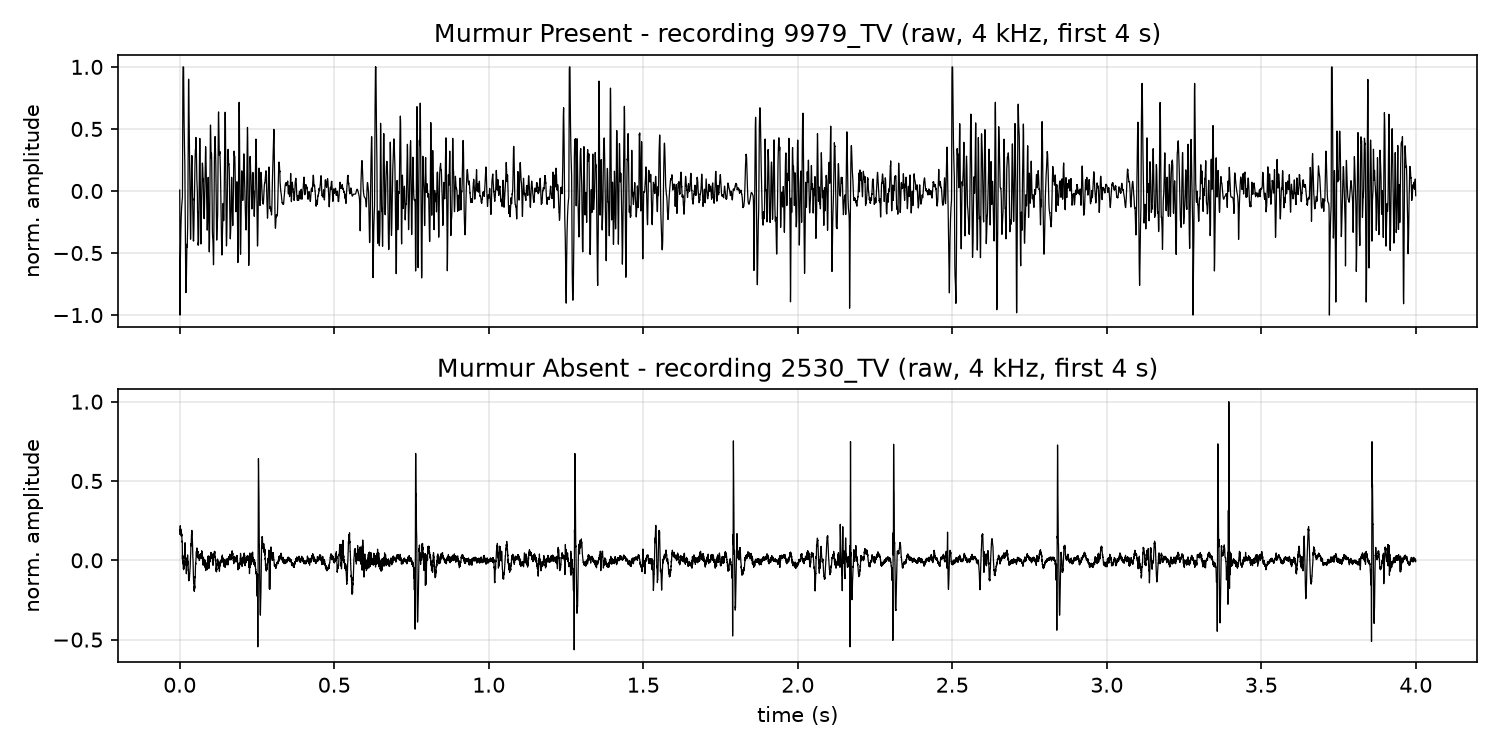
\includegraphics[width=0.49\textwidth]{fig1_raw_pcg_present_vs_absent.png}\hfill
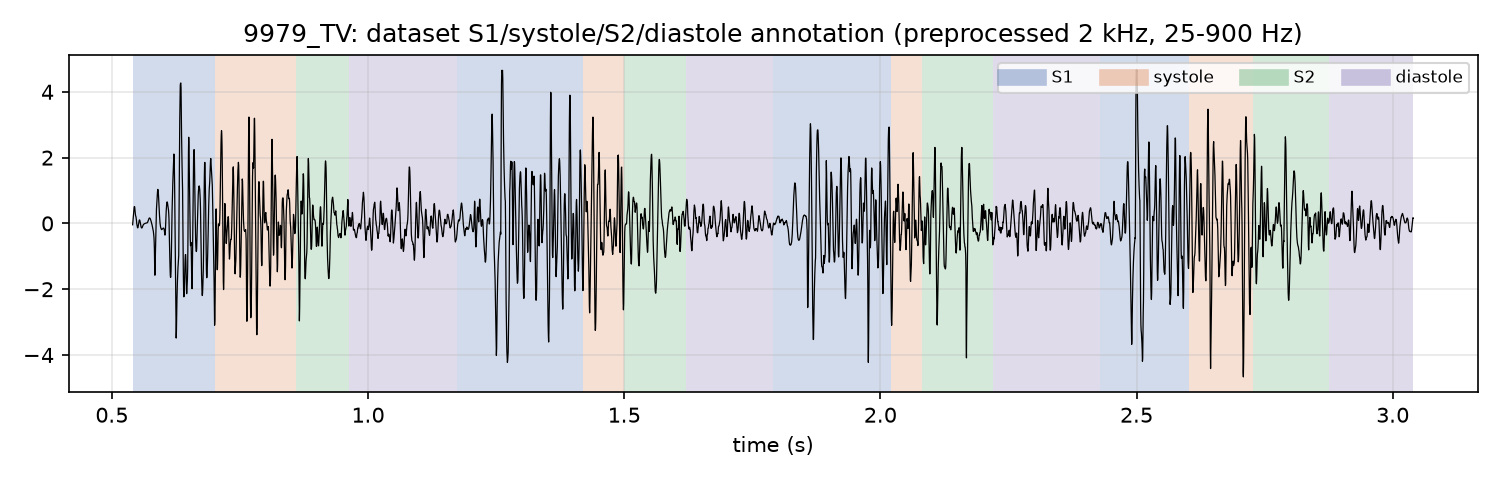
\includegraphics[width=0.49\textwidth]{fig3_annotated_cycles.png}
\caption{Left: raw PCG of a murmur-present and a murmur-absent recording. Right: expert S1/systole/S2/diastole annotation
of the cardiac cycles (CirCor \texttt{.tsv}). Phase-1 figures.}\label{fig:signals}
\end{figure}

\section{Signal-processing methodology}
Every recording is resampled to 2\,kHz (polyphase FIR), band-pass filtered at 25--900\,Hz (zero-phase Butterworth, order 4)
and z-scored; no statistic is estimated across recordings. Figure~\ref{fig:pipe} shows the pipeline.
\begin{figure}[H]\centering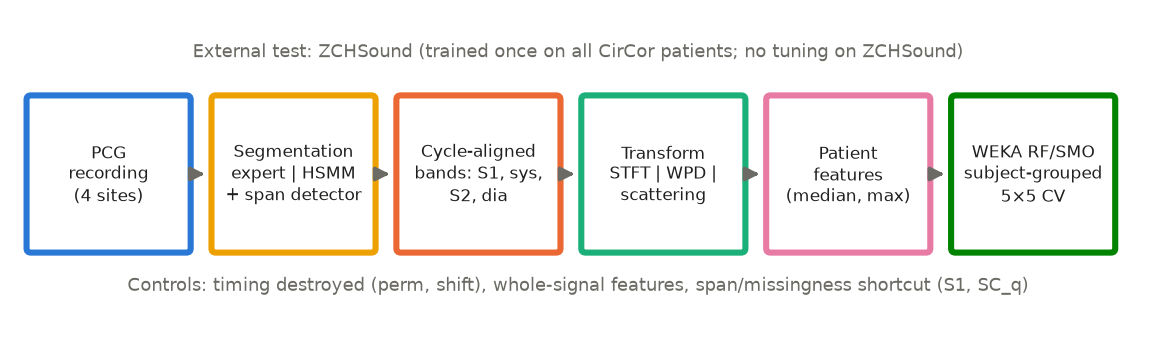
\includegraphics[width=\textwidth]{fig_pipeline.png}
\caption{Pipeline and controls.}\label{fig:pipe}\end{figure}

\subsection{Wavelet transform mathematics}
A signal $x$ is represented in an orthonormal wavelet basis by scaling functions $\phi_{J,k}$ and wavelets $\psi_{j,k}$,
\begin{equation}
x(t)=\sum_k c_{J,k}\,\phi_{J,k}(t)+\sum_{j=1}^{J}\sum_k d_{j,k}\,\psi_{j,k}(t),\qquad
\psi_{j,k}(t)=2^{-j/2}\psi(2^{-j}t-k).
\end{equation}
The discrete wavelet transform (DWT) computes the coefficients with a two-channel filter bank: with low-pass filter $h$ and
high-pass filter $g[n]=(-1)^n h[L-1-n]$,
\begin{equation}
a_{j+1}[k]=\sum_n h[n-2k]\,a_j[n],\qquad d_{j+1}[k]=\sum_n g[n-2k]\,a_j[n],
\end{equation}
starting from $a_0=x$. Each level halves the band and the sampling rate, so the DWT refines only the low-frequency
branch (Figure~\ref{fig:dwt}). We use the Daubechies db4 filter (length 8), fixed before any result for its time
localisation over the 100--300\,ms systolic interval; db6, sym8 and coif3 were sensitivity analyses only.

\subsection{Wavelet-packet decomposition}
The wavelet packet decomposition (WPD) splits \emph{both} the approximation and the detail branch at every level. At
depth $J$ it yields $2^J$ nodes; ordered by frequency, node $b$ covers approximately
$[\,b\,f_s/2^{J+1},\,(b+1)\,f_s/2^{J+1})$. With $f_s=2$\,kHz and $J=4$ this gives 16 bands of 62.5\,Hz between 0 and
1\,kHz on an 8\,ms grid (periodisation mode). Band energy maps $E_b(t)$ are the squared node coefficients. Real filters
leak between neighbouring bands (Figure~\ref{fig:packets}); the STFT comparison below uses the same nominal band edges, so
leakage is part of what is compared.
\begin{figure}[H]\centering
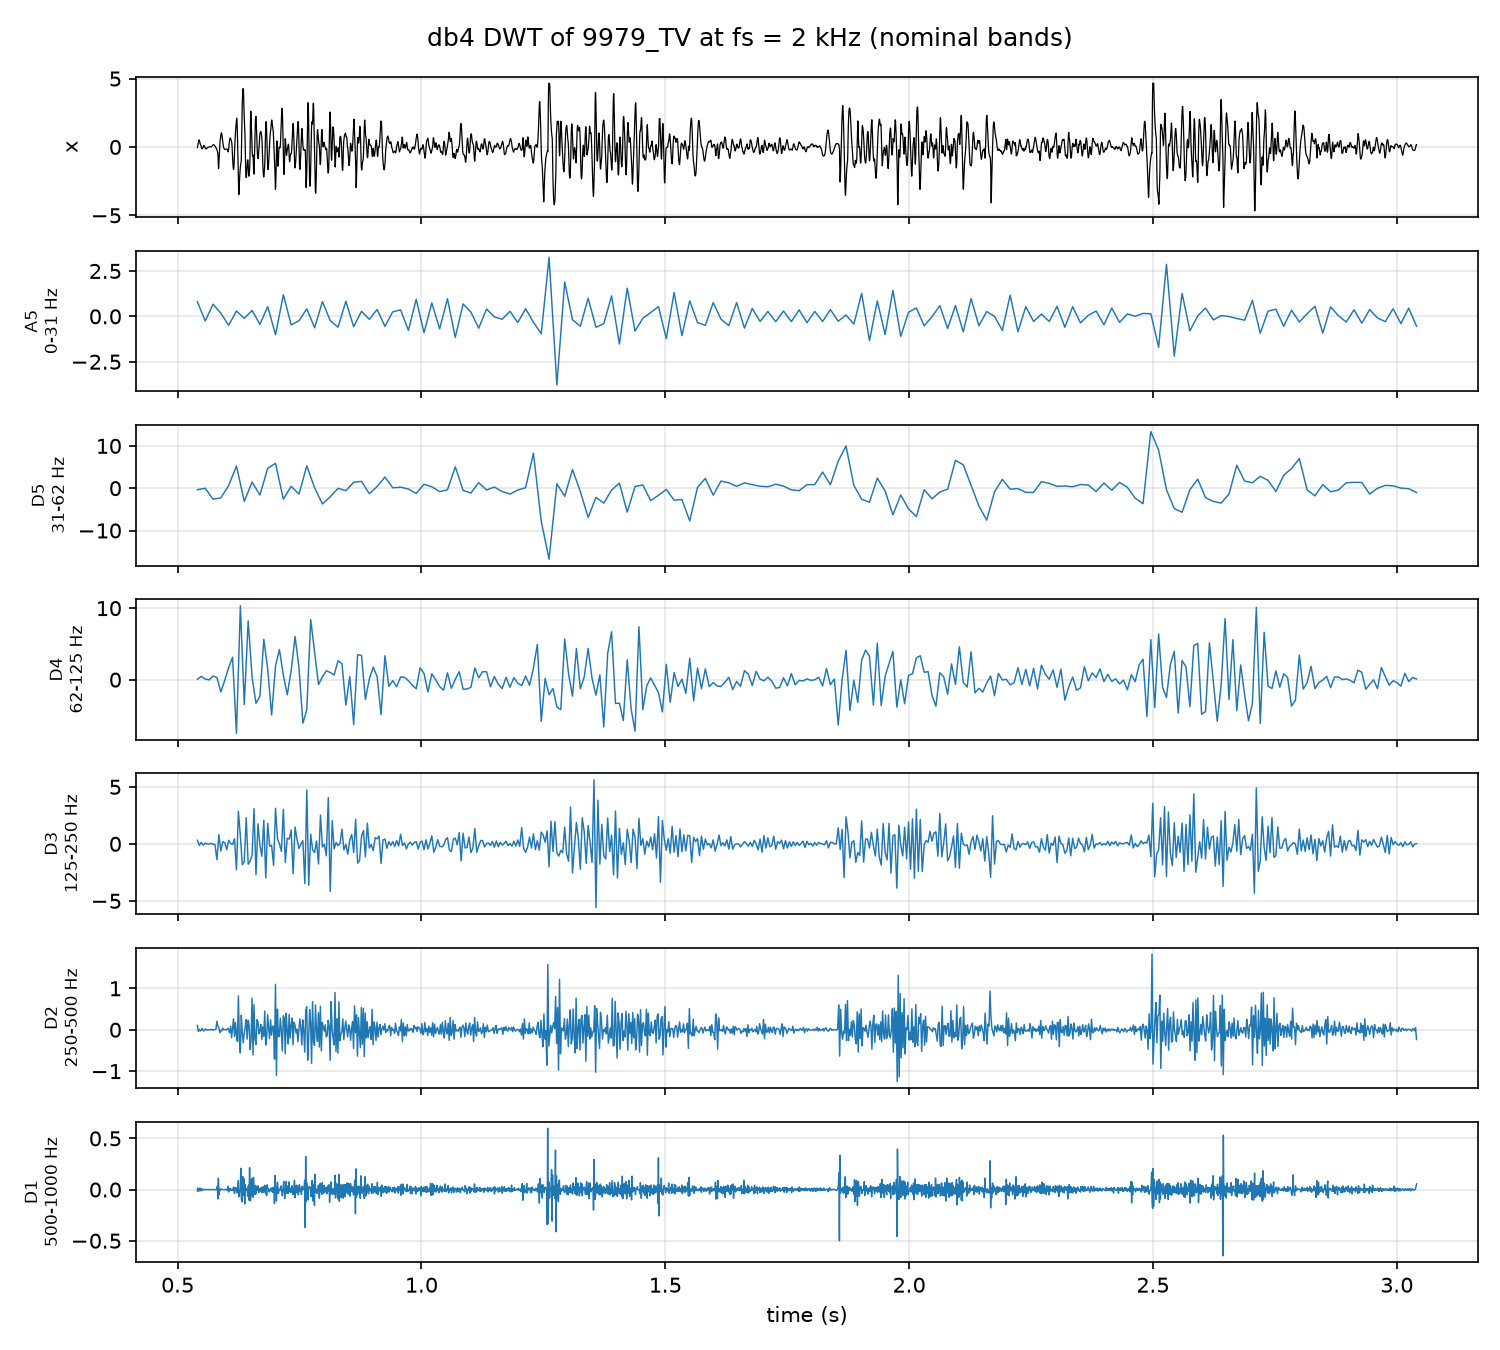
\includegraphics[width=0.49\textwidth]{fig4_dwt_decomposition.png}\hfill
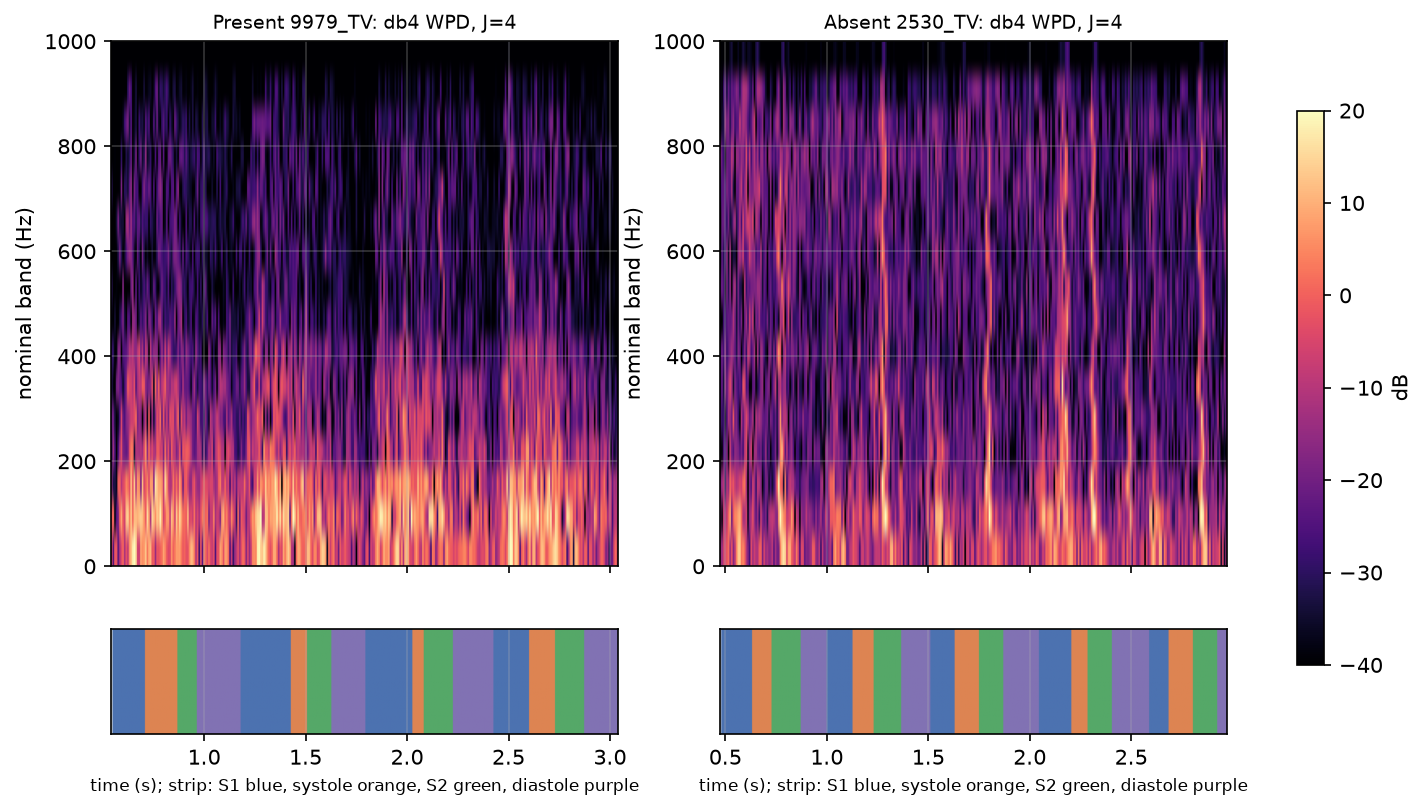
\includegraphics[width=0.49\textwidth]{fig5_wpd_time_frequency.png}
\caption{Left: DWT decomposition of a PCG. Right: depth-4 WPD time--frequency energy map. Phase-1 figures.}\label{fig:dwt}
\end{figure}
\begin{figure}[H]\centering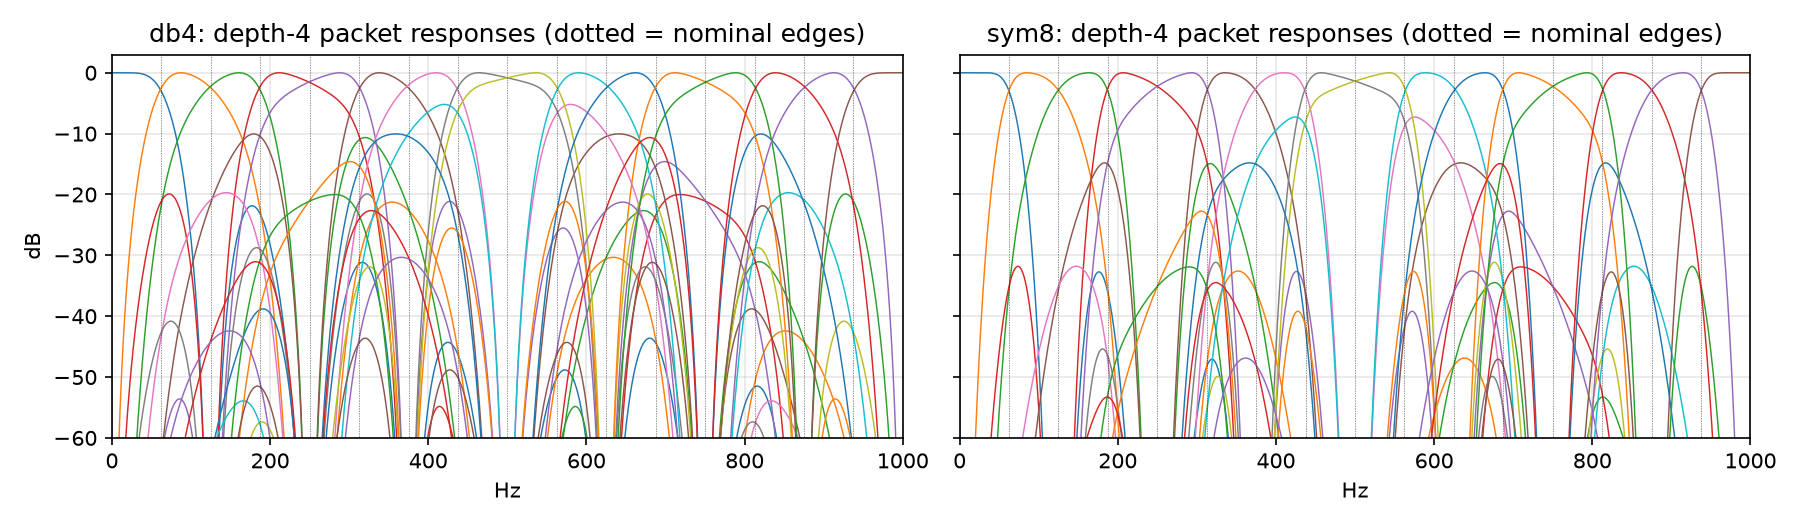
\includegraphics[width=0.85\textwidth]{fig7_packet_frequency_responses.png}
\caption{Frequency responses of the 16 depth-4 packets for db4 and sym8 (dotted: nominal edges).}\label{fig:packets}\end{figure}

\subsection{STFT comparison}
The STFT $X(m,\omega)=\sum_n x[n]\,w[n-mR]\,e^{-j\omega n}$ (Hann window $w$, hop $R$) is pooled into the \emph{same} 16
frequency bands on the \emph{same} time grid, giving band energy maps of identical dimension. Hence ``WPD vs STFT''
changes only the transform. \emph{wpds} is WPD with the STFT's Hann window applied as temporal smoothing, which tests
whether a difference is only estimator variance (post-hoc in Phase 1, pre-registered in Phase 2). Wavelet scattering
\cite{anden2014} (kymatio \cite{andreux2020}, $J=6$, $Q=(8, 1)$, first and first+second order) was added in Phase 3 under
the same band features.

\subsection{Features}
\emph{Whole-signal} (W): per band, log relative band energy and log$(q_{90}/q_{50})$ burstiness, plus two entropies.
\emph{Cycle-aligned} (A, E2, E4): per band, log(systolic energy / S1 energy) and log(systolic / diastolic energy), plus two
entropies. A recording contributes aligned features only if enough systole, diastole and S1 are annotated; otherwise they
are missing (recorded, not imputed silently). Patient vector: median and maximum over the patient's recordings.
Baselines: B0 (MFCC and spectral descriptors) and B1, the 2025 wavelet baseline \cite{vimalajeewa2025}, re-implemented from
the authors' code.

\section{Cardiac-cycle segmentation}
\begin{itemize}\setlength\itemsep{1pt}
\item \textbf{Expert labels} (E2 \texttt{true}): the CirCor \texttt{.tsv} annotation. Results using it at test time are
\emph{oracle-conditioned}. Controls keep the features and destroy timing: \texttt{perm} permutes the labels within a
recording, \texttt{shift} shifts them circularly.
\item \textbf{E1}: homomorphic-envelope peak picking, constants fixed before the run.
\item \textbf{E1b}: a Python port of the logistic-regression HSMM of Springer et al.\ \cite{springer2016}, trained on the
training folds and applied to whole recordings.
\item \textbf{E4}: the LR-HSMM plus a learned span detector (logistic regression on six features of 1-s windows) that keeps
windows likely to be annotatable; trained on the training folds only.
\item \textbf{E4q} (Phase 3): E4 with the same fraction of windows kept in every recording, which removes the
span-fraction shortcut by construction.
\item \textbf{Diagnostics D1--D3} use the expert spans at test time (labelled as such): HSMM timing inside expert spans
(D1), timing destroyed inside spans (D2), whole-signal features inside spans (D3).
\end{itemize}

\section{WEKA classification}
All classifiers are WEKA 3.9.7 \cite{frank2016}, called in batch from Python: RandomForest \cite{breiman2001}
(\texttt{-I 300 -K 0 -S 1 -num-slots 1}; primary), SMO \cite{platt1998} with a linear PolyKernel and logistic calibration
(secondary), and MLP and Logistic in Phase 1. WEKA's own cross-validation is never used, because it splits rows and would
put recordings of the same child in training and test data. One fold reproduced with the WEKA command line equals the
pipeline's predictions exactly (\nm{wekaDemoNTrain} training and \nm{wekaDemoNTest} test patients;
\texttt{weka\_demo/}).

\section{Experimental protocol}
Folds: 5 repeats $\times$ 5 outer folds, subject-grouped and stratified, fixed before any model ran (sha256
\texttt{c4aa74c7\ldots2339}). Thresholds are chosen on inner training folds only (specificity $\geq 0.80$). Phase 1 (v1)
was locked before any result; Phase 2 (E0--E4, D1--D3, S1) and Phase 3 (G1--G4) were each pre-registered with fixed
decision rules before their runs, but after the preceding results on the same folds (sequential design). Deviations are
dated amendments committed before the affected run.

\section{Evaluation metrics}
\textbf{Patient AUROC}, the probability that a random Present patient scores higher than a random Absent patient. We report
two definitions and never mix them: the \emph{mean of repeat AUROCs} ($\pm$ SD over the 5 repeats), and the \emph{AUROC
of repeat-averaged scores}, where each patient's out-of-fold score is averaged over the repeats; the latter is used by
every hypothesis test, with a 95\,\% subject-bootstrap CI (2000 resamples). At the operating point we report sensitivity
(Se), specificity (Sp) and the Challenge weighted accuracy, which in the binary encoding is
\begin{equation}
\mathrm{W.acc}=\frac{5\,\mathrm{TP}+\mathrm{TN}}{5\,(\mathrm{TP}+\mathrm{FN})+(\mathrm{TN}+\mathrm{FP})}.
\end{equation}
\textbf{Decision rules} (registered per hypothesis): typically $\Delta\geq0.03$, CI lower bound $>0$ and at least 18/25
folds with $\Delta>0$. H6a, H8a and H9a used a point-estimate criterion $\Delta\geq-0.03$; it is \emph{not} a formal
non-inferiority test.

\section{Results}\label{sec:res}
Table~\ref{tab:main} summarises the reference models. Cycle-aligned WPD beats whole-signal WPD (H3: \nm{hypH3WpdFull}) and
the re-evaluated 2025 baseline B1 (H4b: \nm{hypH4bWpdFull}), but not B0 (H4a: \nm{hypH4aWpdFull}). Figure~\ref{fig:roc} shows
the patient ROC curves.
\begin{table}[H]\centering\caption{Main models (RF, patient level, AUROC of repeat-averaged scores; operating point:
inner-fold threshold for specificity $\geq 0.80$; W.acc at that threshold).}\label{tab:main}
\resizebox{0.9\textwidth}{!}{\begin{tabular}{@{}lcccc@{}}
\toprule
Model (RF) & AUROC [95\,\% CI] & Se & Sp & W.acc \\
\midrule
B0 acoustic baseline & \nm{v1B0RFAucFull} & \nm{opReproMacB0RFSens} & \nm{opReproMacB0RFSpec} & \nm{opReproMacB0RFWacc} \\
B1 Vimalajeewa et al. & \nm{v1B1RFAucFull} & \nm{opReproMacB1RFSens} & \nm{opReproMacB1RFSpec} & \nm{opReproMacB1RFWacc} \\
whole-signal STFT (W\_stft) & \nm{decWholeStftFull} & \nm{opReproMacWStftRFSens} & \nm{opReproMacWStftRFSpec} & \nm{opReproMacWStftRFWacc} \\
expert-aligned STFT (oracle) & \nm{decExpertStftFull} & \nm{opE2E2StftTrueRFSens} & \nm{opE2E2StftTrueRFSpec} & \nm{opE2E2StftTrueRFWacc} \\
E4 automatic STFT & \nm{decEFourStftFull} & \nm{opE4E4StftRFSens} & \nm{opE4E4StftRFSpec} & \nm{opE4E4StftRFWacc} \\
E4q shortcut-free STFT & \nm{gTwoAucE4qStftFull} & \nm{opP3G2E4qStftRFSens} & \nm{opP3G2E4qStftRFSpec} & \nm{opP3G2E4qStftRFWacc} \\
\bottomrule
\end{tabular}
}\end{table}
\begin{figure}[H]\centering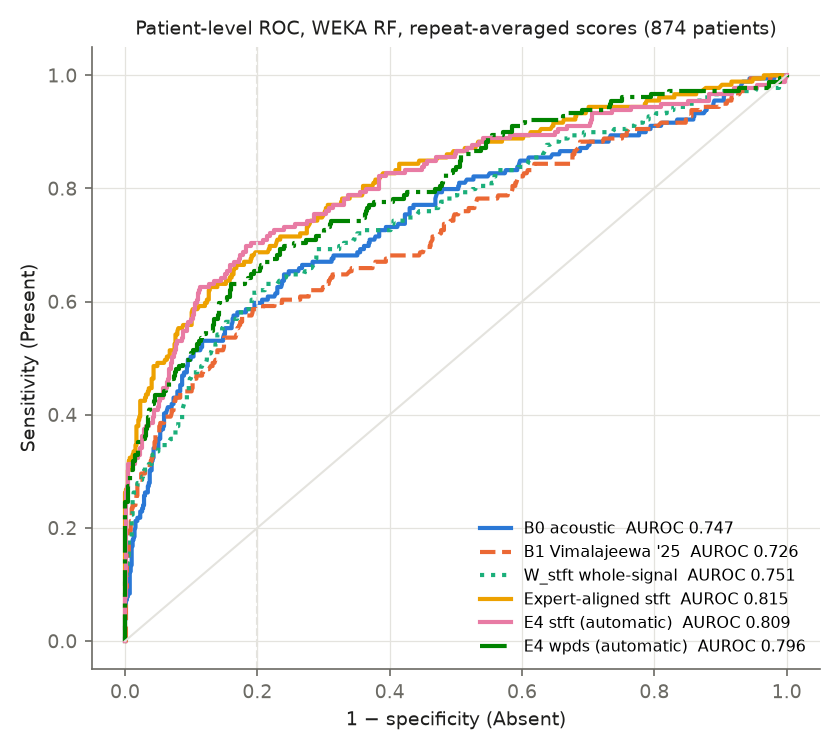
\includegraphics[width=0.75\textwidth]{fig_final_roc.png}
\caption{Patient-level ROC (RF, repeat-averaged scores).}\label{fig:roc}\end{figure}

\subsection{Ablation: timing versus span choice}
With expert labels, destroying timing costs \nm{hFivePermRange} AUROC (\texttt{perm}, H5a--c) and \nm{hFiveShiftRange}
(\texttt{shift}, H5d), all in 25/25 folds. The diagnostics split this exactly (Figure~\ref{fig:dec}): within-span timing is
worth \nm{decDiffWithinSpanTimingRange}, and span selection without timing contributes \nm{decDiffSpanSelNoTimingRange}.
This decomposition is against the timing-destroyed null; it does not mean that alignment explains every difference
between models.
\begin{figure}[H]\centering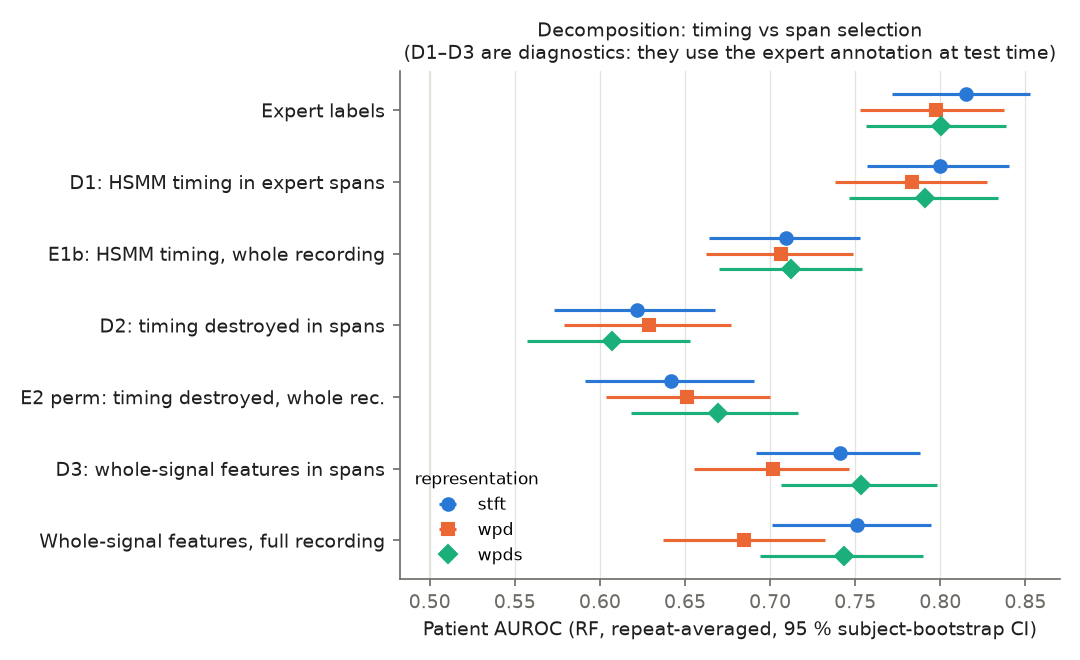
\includegraphics[width=0.85\textwidth]{fig_final_decomposition.png}
\caption{Decomposition of the expert-label result (RF AUROC, 95\,\% CI). D1--D3 use the expert annotation at test time.}\label{fig:dec}\end{figure}

\subsection{Wavelet versus Fourier}
Under every labelling, WPD and smoothed WPD are at most equal to matched STFT bands (Figure~\ref{fig:wvs}; H2a:
\nm{hypH2aWpdFull}; H2b, whole signal: \nm{hypH2bWpdFull}); equivalence within $\pm0.03$ is not shown
(\nm{hypEquivalenceWpdsFull}). Wavelet scattering does not beat STFT bands either (Figure~\ref{fig:scat}; H11a
\nm{gFourH11aAScat1AStftFull}, H11b \nm{gFourH11bAScat12AStftFull}); second-order paths add \nm{gFourH11cAScat12AScat1Full},
below the registered 0.03.
\begin{figure}[H]\centering
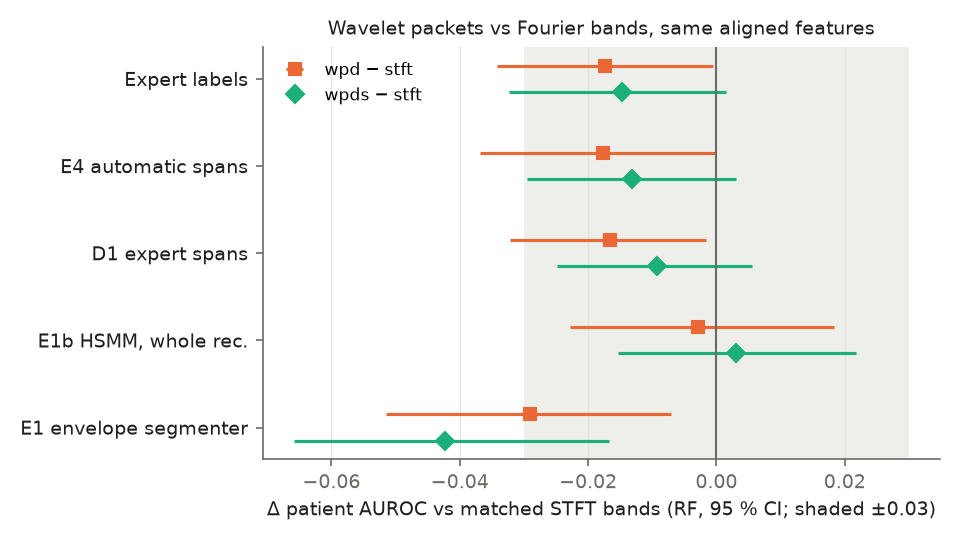
\includegraphics[width=0.56\textwidth]{fig_final_wavelet_vs_stft.png}\hfill
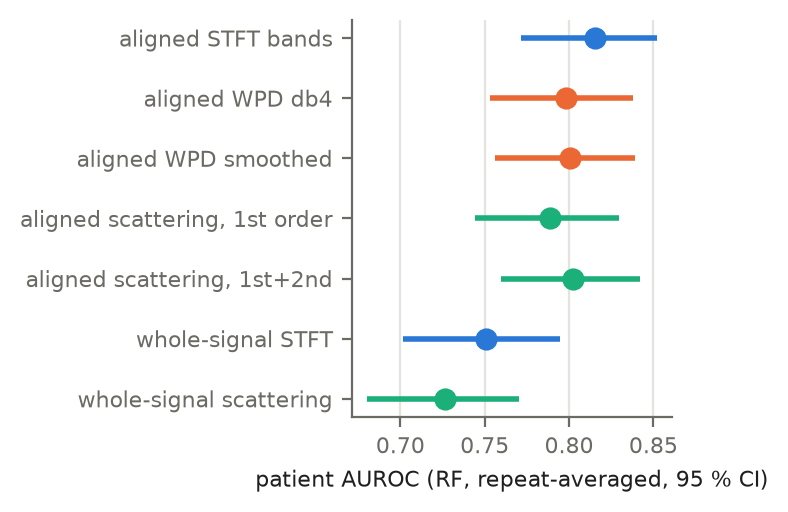
\includegraphics[width=0.42\textwidth]{fig_scattering.png}
\caption{Left: WPD minus matched STFT bands under each labelling (shaded $\pm0.03$). Right: STFT, WPD and scattering features (RF AUROC).}\label{fig:wvs}\label{fig:scat}\end{figure}

\subsection{Failed hypotheses}
Reported in full in Appendix~\ref{app:hyp}. Not supported: H1 (no material inflation from random splits in the authors'
recording-level setting), H2a/H2b (no wavelet advantage), H4a (no gain over B0), every E1 and E1b hypothesis (H6, H8),
H9c for the primary wpd, H11a--c (scattering), and H12a (shortcut-free advantage). The planned soft-murmur experiment (H7)
was dropped by amendment before it ran.

\subsection{Automatic-segmentation analysis}
Envelope peaks (E1) and the LR-HSMM on whole recordings (E1b) miss their targets (e.g.\ H8a \nm{hypH8aWpdFull}). The HSMM's
timing is close to expert timing inside expert spans (expert $-$ D1: \nm{decDiffHsmmTimingErrorRange}); what is missing is
span selection (D1 $-$ E1b: \nm{decDiffSpanSelHsmmRange}). With the learned span detector (E4) the point estimate is within
the pre-registered $-0.03$ of expert labels (H9a: \nm{hypH9aWpdFull} for wpd), but the CI lower bound is below $-0.03$, so
statistical non-inferiority is \textbf{not established}. E4 beats B1 (H9b: \nm{hNineBRange}). Table~\ref{tab:g3a} gives the
cost of replacing the expert segmentation by each automatic one (conditioning gaps, \cite{cao2026}).
\begin{table}[H]\centering\caption{Conditioning gaps: AUROC(expert) minus AUROC(estimated or random) (RF, 95\,\% CI).}\label{tab:g3a}
\resizebox{0.85\textwidth}{!}{\begin{tabular}{@{}lccc@{}}
\toprule
Gap (RF AUROC) & stft & wpd & wpds \\
\midrule
$\Delta_{or}$ expert $-$ perm & \nm{gThreeAE2StftPermFull} & \nm{gThreeAE2WpdPermFull} & \nm{gThreeAE2WpdsPermFull} \\
$\Delta_{or}$ expert $-$ shift & \nm{gThreeAE2StftShiftFull} & \nm{gThreeAE2WpdShiftFull} & \nm{gThreeAE2WpdsShiftFull} \\
$\Delta_{oe}$ expert $-$ E1 & \nm{gThreeAE1StftAutoFull} & \nm{gThreeAE1WpdAutoFull} & \nm{gThreeAE1WpdsAutoFull} \\
$\Delta_{oe}$ expert $-$ E1b & \nm{gThreeAE1bStftAutoFull} & \nm{gThreeAE1bWpdAutoFull} & \nm{gThreeAE1bWpdsAutoFull} \\
$\Delta_{oe}$ expert $-$ E4 & \nm{gThreeAE4StftFull} & \nm{gThreeAE4WpdFull} & \nm{gThreeAE4WpdsFull} \\
$\Delta_{oe}$ expert $-$ E4q & \nm{gThreeAE4qStftFull} & \nm{gThreeAE4qWpdFull} & \nm{gThreeAE4qWpdsFull} \\
\bottomrule
\end{tabular}
}\end{table}

\subsection{Shortcut-learning investigation}
E4's selected-span fraction alone predicts the class (AUROC \nm{eFourShortcutPredFrac}, post-hoc check). Against plain
whole-signal STFT, the H9c rule is met for stft (\nm{hypH9cStftFull}) but not for the primary wpd (\nm{hypH9cWpdFull}). When
whole-signal STFT is given the same span and missingness variables (S1), E4's margin is \nm{sOneWstftRange} with CIs that
include zero. The shortcut-free E4q removes the shortcut (shortcut variables alone: \nm{gTwoAucG2SCqOnlyFull}; test
recordings without aligned features fall from \nm{gTwoNofeatE4RAbsent}\,\% to \nm{gTwoNofeatE4qAbsent}\,\% for Absent
patients) at essentially no cost (E4q $-$ E4: \nm{gTwoDescStftE4StftFull}), and learned selection beats random windows
(H12b: \nm{gTwoH12bStftFull}). Its margin over whole-signal STFT with the same information is \nm{gTwoH12aStftFull}
(H12a): the CI includes zero, so this advantage is \textbf{not established}.

\subsection{External test on ZCHSound}
A whole-signal STFT model trained once on all 874 CirCor patients was applied unchanged to ZCHSound (Figure~\ref{fig:ext},
Table~\ref{tab:ext}). On the clean set the any-CHD AUROC is \nm{hTenAFull} (H10a supported; internal CirCor
\nm{zchWStftRFAllCleanInternal}). By subtype: PDA \nm{zchSubWStftRFPDAFull}, VSD \nm{zchSubWStftRFVSDFull}, ASD
\nm{zchSubWStftRFASDFull}, PFO \nm{zchSubWStftRFPFOFull}, the pre-registered physiological order (H10b: VSD $-$ PFO
\nm{hTenBvsdPfoFull}). On the noisy neonatal set the AUROC is \nm{zchWStftRFAllNoisyFull} (chance). A post-hoc check shows
that the score is unrelated to age (Spearman \nm{ageWStftRFAllRho}).
\begin{figure}[H]\centering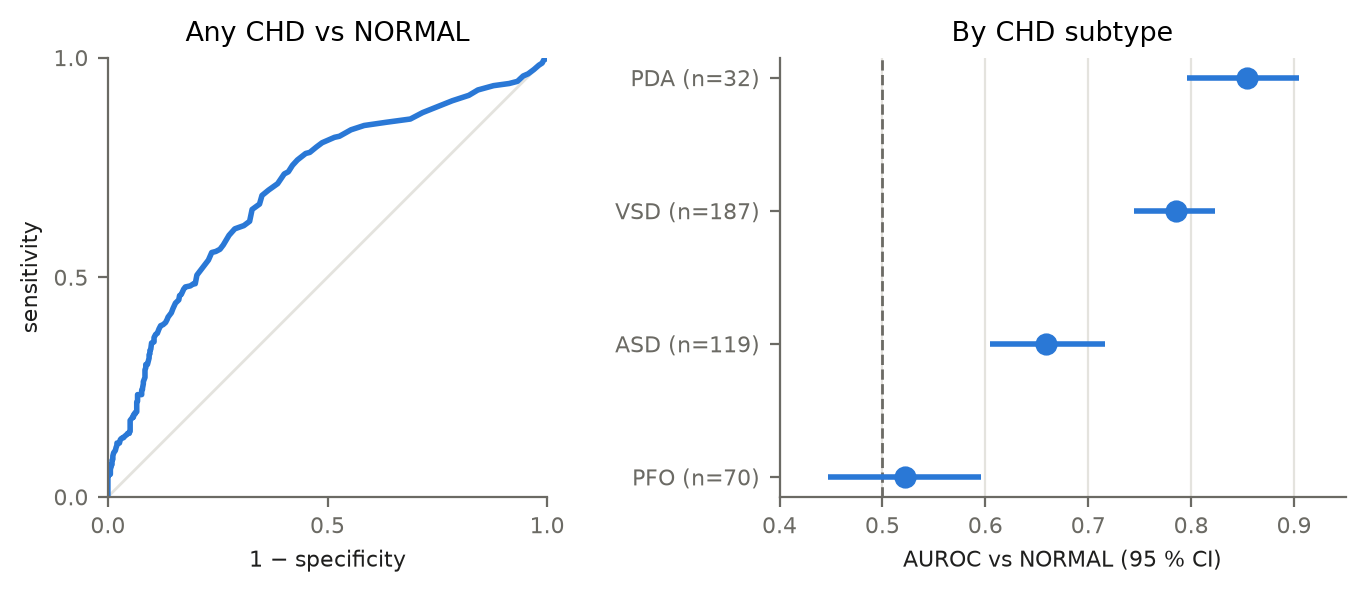
\includegraphics[width=0.92\textwidth]{fig_external.png}
\caption{ZCHSound clean set, RF W\_stft trained on CirCor: any-CHD ROC and AUROC by subtype vs NORMAL (95\,\% CI).}\label{fig:ext}\end{figure}
\begin{table}[H]\centering\caption{External AUROC for any CHD (RF). B0 enters no verdict: its external signal is an artefact.}\label{tab:ext}
\resizebox{0.85\textwidth}{!}{\begin{tabular}{@{}lccc@{}}
\toprule
Model (RF, trained on CirCor) & clean & noisy & CirCor internal \\
\midrule
W\_stft (pre-registered, H10a) & \nm{zchWStftRFAllCleanFull} & \nm{zchWStftRFAllNoisyFull} & \nm{zchWStftRFAllCleanInternal} \\
W\_wpd\_db4\_smooth & \nm{zchWWpdDb4SmoothRFAllCleanFull} & \nm{zchWWpdDb4SmoothRFAllNoisyFull} & \nm{zchWWpdDb4SmoothRFAllCleanInternal} \\
W\_scat1 & \nm{zchWScat1RFAllCleanFull} & \nm{zchWScat1RFAllNoisyFull} & \nm{zchWScat1RFAllCleanInternal} \\
B0 (artefact, no verdict) & \nm{zchB0RFAllCleanFull} & \nm{zchB0RFAllNoisyFull} & \nm{zchB0RFAllCleanInternal} \\
\bottomrule
\end{tabular}
}\end{table}

\subsection{Comparison with recent work}
Only B1 \cite{vimalajeewa2025} was re-evaluated on our data and folds; on that common scale our aligned and automatic
models are better (H4b, H9b). The higher numbers in Table~\ref{tab:lit} are not comparable with ours. For example,
Nogueira et al.\ \cite{nogueira2026} report (Se+Sp)/2 = \nm{litNogueiraOverall} with test segments that start at expert-annotated
S1 onsets; on the same balanced-accuracy scale our expert-label model reaches \nm{opE2E2StftTrueRFBacc}, E4
\nm{opE4E4StftRFBacc}. Nie et al.\ \cite{nie2024} report snippet-level accuracy on annotated periods and note themselves
that this differs from recording-level Challenge evaluation. In our data the expert segmentation is worth up to
\nm{gThreeAE1bStftAuto} AUROC over a naive automatic pipeline, which illustrates how much test-time conditioning can change a
number.

\section{Critical discussion}
The wavelet experiments are informative even though STFT was at least as good: with matched bands, grid and features, the
transform was the only change. For these features, therefore, the transform itself brings no advantage; a wavelet advantage
reported in other pipelines would need another explanation (for example a different feature design or test-time
conditioning), which we did not test. The strongest effect is timing, but it was measured with
expert labels; making it work automatically needed span selection, and part of that apparent gain is explained by which
spans are kept. The honest summary of the automatic pipeline is therefore ``close to expert labels on the point estimate,
not shown to be better than a shortcut-aware whole-signal baseline''. The external test supports transfer of a simple
whole-signal model across cohorts and devices, with physiologically sensible behaviour (loud shunts detected, silent PFO
not), but it tests a CHD label, not murmur detection.

\section{Limitations}
\begin{itemize}\setlength\itemsep{1pt}
\item Cross-validation on one public cohort; no CirCor hidden test set; no prospective or clinical evaluation.
\item No intrinsic wavelet superiority was demonstrated; STFT bands were at least as good.
\item Aligned results depend on segmentation and span selection; expert-label results are oracle-conditioned.
\item Only 179 Present patients; CIs are wide.
\item Possible shortcut learning in automatic pipelines (S1; H12a not established).
\item The Unknown class is excluded, so the task is easier than the three-class Challenge task.
\item ZCHSound labels are CHD diagnoses, not murmurs; the noisy neonatal subset is at chance.
\item SMO is numerically unstable on scattering features; no SMO scattering number is used as evidence.
\item E1b, E4, S1 and Phase 3 were designed after earlier results on the same folds.
\item Murmur detection is not a clinical-outcome diagnosis; nothing here supports deployment.
\item The systematic literature audit was searched and screened but not coded, so no literature-wide rate is reported.
\end{itemize}

\section{Conclusion}
On CirCor, cardiac-cycle timing carries the murmur information available to these features, and the choice between
wavelet packets, STFT and scattering does not change the result. A whole-signal model transfers to an independent
paediatric CHD cohort with the expected physiological ordering. Future work: signal-quality gating for noisy recordings,
learned models evaluated under the same subject-grouped and shortcut-controlled protocol, a murmur-labelled external set,
and a systematic audit of test-time expert segmentation in published CirCor work.

\section*{Reproducibility statement}
{\sloppy Code, protocols, saved predictions and tables: \url{https://github.com/pm2m1/ec418-circor-research}. Protocol tags
\path{v1.0-pilot}, \path{protocol-v2-lock}, \path{e1b-prereg}, \path{diag-prereg}, \path{e4-prereg},
\path{s1-prereg}; results \path{results-final} and \path{phase3-results}; checksum manifests in
\path{results/v1_freeze/} and \path{results/final_freeze/}; quick verification with
\path{scripts/p5_verify_integrity.py}; full guide \path{docs/REPRODUCIBILITY.md}. Every number in this report is
generated from saved tables (\path{scripts/p4_numbers.py}) and checked by \path{scripts/p4_check_numbers.py}.\par}

\section*{AI-assistance statement}
This project was carried out with substantial assistance from an AI coding assistant (Anthropic's Claude, used through
Claude Code). It wrote most of the code, ran the analyses, drafted this report and the slides, and performed the
literature screening and the transcription of the Google Scholar export. The author defined the study, made the decisions
recorded in the protocols and amendments, and is responsible for the content. \todo{The author should review this report
and restate the findings in their own words before submission.}

\begin{thebibliography}{99}\small
\bibitem{oliveira2022} J.~Oliveira et al., ``The CirCor DigiScope dataset: From murmur detection to murmur classification,'' \emph{IEEE J. Biomed. Health Inform.}, vol.~26, no.~6, pp.~2524--2535, 2022.
\bibitem{goldberger2000} A.~L. Goldberger et al., ``PhysioBank, PhysioToolkit, and PhysioNet,'' \emph{Circulation}, vol.~101, no.~23, pp.~e215--e220, 2000.
\bibitem{reyna2023} M.~A. Reyna et al., ``Heart murmur detection from phonocardiogram recordings: The George B. Moody PhysioNet Challenge 2022,'' \emph{PLOS Digit. Health}, vol.~2, no.~9, e0000324, 2023.
\bibitem{vimalajeewa2025} D.~Vimalajeewa, C.~Lee, B.~Vidaković, ``Multiscale analysis of heart sound signals in the wavelet domain for heart murmur detection,'' \emph{Sci. Rep.}, vol.~15, art.~10315, 2025, doi:10.1038/s41598-025-93989-0.
\bibitem{mcdonald2024} A.~McDonald, M.~Gales, A.~Agarwal, ``A recurrent neural network and parallel hidden Markov model algorithm to segment and detect heart murmurs in phonocardiograms,'' \emph{PLOS Digit. Health}, e0000436, 2024.
\bibitem{springer2016} D.~B. Springer, L.~Tarassenko, G.~D. Clifford, ``Logistic regression-HSMM-based heart sound segmentation,'' \emph{IEEE Trans. Biomed. Eng.}, vol.~63, no.~4, pp.~822--832, 2016.
\bibitem{niizumi2024} D.~Niizumi, D.~Takeuchi, Y.~Ohishi, N.~Harada, K.~Kashino, ``Exploring pre-trained general-purpose audio representations for heart murmur detection,'' in \emph{Proc. IEEE EMBC}, 2024, doi:10.1109/EMBC53108.2024.10782479.
\bibitem{dehghan2024} O.~Dehghan Manshadi, S.~Mihandoost, ``Murmur identification and outcome prediction in phonocardiograms using deep features based on Stockwell transform,'' \emph{Sci. Rep.}, 2024, doi:10.1038/s41598-024-58274-6.
\bibitem{nie2024} J.~Nie, R.~Liu, B.~Mahasseni, E.~Azemi, V.~Mitra, ``Model-driven heart rate estimation and heart murmur detection based on phonocardiogram,'' in \emph{Proc. IEEE MLSP}, 2024 (arXiv:2407.18424).
\bibitem{hong2025} Z.~Hong, W.~Yu, C.~Li, B.~Yang, Z.~Fan, R.~Wei, ``DPPAT: Dual-level periodic pattern-aware transformer for heart sound murmur identification,'' \emph{IEEE J. Biomed. Health Inform.}, 2025, doi:10.1109/JBHI.2025.3638048.
\bibitem{kutlu2026} H.~Kutlu, C.~Çolak, ``Cross-dataset generalization in phonocardiogram murmur classification: A benchmark study of domain-conditional performance and the role of multi-representation fusion,'' \emph{J. Clin. Med.}, vol.~15, no.~20, 2026, doi:10.3390/jcm15208058.
\bibitem{ladislaus2026} N.~D. Ladislaus, D.~E. Olatunji, S.~C. Buol, ``The vote hides the failure: Aggregation choice and noise robustness in heart murmur detection,'' arXiv:2609.37161, 2026.
\bibitem{nogueira2026} M.~Nogueira, J.~H. Oliveira, C.~G. Ferreira, M.~T. Coimbra, A.~M. Jorge, ``Selection of heart sound segments for synchronous classification of multi-channel heart sounds,'' arXiv:2608.21499, 2026.
\bibitem{zewail2026} R.~Zewail, ``Scattering transformer: A training-free transformer architecture for heart murmur detection,'' in \emph{Lecture Notes in Computer Science}, 2026, doi:10.1007/978-3-032-19865-5\_12.
\bibitem{cao2026} D.~P.~M. Cao, H.~D. Pham, H.~Pham, ``When oracle conditioning misleads deployment: Conditioning-availability bias in echocardiographic segmentation,'' arXiv:2608.03342, 2026.
\bibitem{jia2024} Jia et al., ``ZCHSound: Open-source ZJU paediatric heart sound database with congenital heart disease,'' \emph{IEEE Trans. Biomed. Eng.}, vol.~71, no.~8, pp.~2278--2286, 2024, doi:10.1109/TBME.2023.3348800.
\bibitem{anden2014} J.~Andén, S.~Mallat, ``Deep scattering spectrum,'' \emph{IEEE Trans. Signal Process.}, vol.~62, no.~16, pp.~4114--4128, 2014.
\bibitem{andreux2020} M.~Andreux et al., ``Kymatio: Scattering transforms in Python,'' \emph{J. Mach. Learn. Res.}, vol.~21, no.~60, pp.~1--6, 2020.
\bibitem{frank2016} E.~Frank, M.~A. Hall, I.~H. Witten, ``The WEKA Workbench,'' online appendix to \emph{Data Mining: Practical Machine Learning Tools and Techniques}, 4th ed., Morgan Kaufmann, 2016.
\bibitem{breiman2001} L.~Breiman, ``Random forests,'' \emph{Mach. Learn.}, vol.~45, no.~1, pp.~5--32, 2001.
\bibitem{platt1998} J.~Platt, ``Fast training of support vector machines using sequential minimal optimization,'' in \emph{Advances in Kernel Methods}, MIT Press, 1998.
\end{thebibliography}

\appendix
\section{Every pre-registered hypothesis}\label{app:hyp}
\begin{table}[H]\centering\caption{All pre-registered hypotheses (RF, AUROC of repeat-averaged patient scores, subject-bootstrap 95\,\% CI). ``SUPPORTED'' for H6a/H8a/H9a means that the point-estimate rule was met.}
\resizebox{\textwidth}{!}{\begin{tabular}{@{}llccl@{}}
\toprule
Hyp. & Contrast (RF) & $\Delta$ AUROC [95\,\% CI] & folds $>0$ & verdict \\
\midrule
H1 & B1+SVM recording AUC: random split - subject-grouped & \nm{hypH1Full} & \nm{hypH1Folds} & \nm{hypH1Verdict} \\
H2a & A\_wpd\_db4 - A\_stft & \nm{hypH2aWpdFull} & \nm{hypH2aWpdFolds} & \nm{hypH2aWpdVerdict} \\
H2b & W\_wpd\_db4 - W\_stft & \nm{hypH2bWpdFull} & \nm{hypH2bWpdFolds} & \nm{hypH2bWpdVerdict} \\
H3 & A\_wpd\_db4 - W\_wpd\_db4 & \nm{hypH3WpdFull} & \nm{hypH3WpdFolds} & \nm{hypH3WpdVerdict} \\
H4a & A\_wpd\_db4 - B0 & \nm{hypH4aWpdFull} & \nm{hypH4aWpdFolds} & \nm{hypH4aWpdVerdict} \\
H4b & A\_wpd\_db4 - B1 & \nm{hypH4bWpdFull} & \nm{hypH4bWpdFolds} & \nm{hypH4bWpdVerdict} \\
H5a & E2\_wpd\_true - E2\_wpd\_perm & \nm{hypH5aWpdFull} & \nm{hypH5aWpdFolds} & \nm{hypH5aWpdVerdict} \\
H5b & E2\_stft\_true - E2\_stft\_perm & \nm{hypH5bStftFull} & \nm{hypH5bStftFolds} & \nm{hypH5bStftVerdict} \\
H5c & E2\_wpds\_true - E2\_wpds\_perm & \nm{hypH5cWpdsFull} & \nm{hypH5cWpdsFolds} & \nm{hypH5cWpdsVerdict} \\
H5d & E2\_wpd\_true - E2\_wpd\_shift & \nm{hypH5dWpdFull} & \nm{hypH5dWpdFolds} & \nm{hypH5dWpdVerdict} \\
H5d & E2\_stft\_true - E2\_stft\_shift & \nm{hypH5dStftFull} & \nm{hypH5dStftFolds} & \nm{hypH5dStftVerdict} \\
H5d & E2\_wpds\_true - E2\_wpds\_shift & \nm{hypH5dWpdsFull} & \nm{hypH5dWpdsFolds} & \nm{hypH5dWpdsVerdict} \\
H6a & E1\_wpd\_auto - E2\_wpd\_true & \nm{hypH6aWpdFull} & \nm{hypH6aWpdFolds} & \nm{hypH6aWpdVerdict} \\
H6b & E1\_wpd\_auto - B1 & \nm{hypH6bWpdFull} & \nm{hypH6bWpdFolds} & \nm{hypH6bWpdVerdict} \\
H6c(a) & E1\_stft\_auto - E2\_stft\_true & \nm{hypH6cAStftFull} & \nm{hypH6cAStftFolds} & \nm{hypH6cAStftVerdict} \\
H6c(b) & E1\_stft\_auto - B1 & \nm{hypH6cBStftFull} & \nm{hypH6cBStftFolds} & \nm{hypH6cBStftVerdict} \\
H6c(a) & E1\_wpds\_auto - E2\_wpds\_true & \nm{hypH6cAWpdsFull} & \nm{hypH6cAWpdsFolds} & \nm{hypH6cAWpdsVerdict} \\
H6c(b) & E1\_wpds\_auto - B1 & \nm{hypH6cBWpdsFull} & \nm{hypH6cBWpdsFolds} & \nm{hypH6cBWpdsVerdict} \\
H8a & E1b\_wpd\_auto - E2\_wpd\_true & \nm{hypH8aWpdFull} & \nm{hypH8aWpdFolds} & \nm{hypH8aWpdVerdict} \\
H8b & E1b\_wpd\_auto - B1 & \nm{hypH8bWpdFull} & \nm{hypH8bWpdFolds} & \nm{hypH8bWpdVerdict} \\
H8c(a) & E1b\_stft\_auto - E2\_stft\_true & \nm{hypH8cAStftFull} & \nm{hypH8cAStftFolds} & \nm{hypH8cAStftVerdict} \\
H8c(b) & E1b\_stft\_auto - B1 & \nm{hypH8cBStftFull} & \nm{hypH8cBStftFolds} & \nm{hypH8cBStftVerdict} \\
H8c(a) & E1b\_wpds\_auto - E2\_wpds\_true & \nm{hypH8cAWpdsFull} & \nm{hypH8cAWpdsFolds} & \nm{hypH8cAWpdsVerdict} \\
H8c(b) & E1b\_wpds\_auto - B1 & \nm{hypH8cBWpdsFull} & \nm{hypH8cBWpdsFolds} & \nm{hypH8cBWpdsVerdict} \\
H9a & E4\_wpd - E2\_wpd\_true & \nm{hypH9aWpdFull} & \nm{hypH9aWpdFolds} & \nm{hypH9aWpdVerdict} \\
H9b & E4\_wpd - B1 & \nm{hypH9bWpdFull} & \nm{hypH9bWpdFolds} & \nm{hypH9bWpdVerdict} \\
H9c & E4\_wpd - W\_stft & \nm{hypH9cWpdFull} & \nm{hypH9cWpdFolds} & \nm{hypH9cWpdVerdict} \\
H9a & E4\_stft - E2\_stft\_true & \nm{hypH9aStftFull} & \nm{hypH9aStftFolds} & \nm{hypH9aStftVerdict} \\
H9b & E4\_stft - B1 & \nm{hypH9bStftFull} & \nm{hypH9bStftFolds} & \nm{hypH9bStftVerdict} \\
H9c & E4\_stft - W\_stft & \nm{hypH9cStftFull} & \nm{hypH9cStftFolds} & \nm{hypH9cStftVerdict} \\
H9a & E4\_wpds - E2\_wpds\_true & \nm{hypH9aWpdsFull} & \nm{hypH9aWpdsFolds} & \nm{hypH9aWpdsVerdict} \\
H9b & E4\_wpds - B1 & \nm{hypH9bWpdsFull} & \nm{hypH9bWpdsFolds} & \nm{hypH9bWpdsVerdict} \\
H9c & E4\_wpds - W\_stft & \nm{hypH9cWpdsFull} & \nm{hypH9cWpdsFolds} & \nm{hypH9cWpdsVerdict} \\
equivalence & E2\_wpds\_true - E2\_stft\_true & \nm{hypEquivalenceWpdsFull} & \nm{hypEquivalenceWpdsFolds} & \nm{hypEquivalenceWpdsVerdict} \\
H7 & soft murmurs (grade I/VI sensitivity) & -- & \nm{hypH7Folds} & \nm{hypH7Verdict} \\
S1(a) & E4\_stft - S1\_Wstft\_SC & \nm{hypS1AStftWstftFull} & \nm{hypS1AStftWstftFolds} & \nm{hypS1AStftWstftVerdict} \\
S1(a) & E4\_stft - S1\_Wwpd\_SC & \nm{hypS1AStftWwpdFull} & \nm{hypS1AStftWwpdFolds} & \nm{hypS1AStftWwpdVerdict} \\
S1(a) & E4\_wpd - S1\_Wstft\_SC & \nm{hypS1AWpdWstftFull} & \nm{hypS1AWpdWstftFolds} & \nm{hypS1AWpdWstftVerdict} \\
S1(a) & E4\_wpd - S1\_Wwpd\_SC & \nm{hypS1AWpdWwpdFull} & \nm{hypS1AWpdWwpdFolds} & \nm{hypS1AWpdWwpdVerdict} \\
S1(a) & E4\_wpds - S1\_Wstft\_SC & \nm{hypS1AWpdsWstftFull} & \nm{hypS1AWpdsWstftFolds} & \nm{hypS1AWpdsWstftVerdict} \\
S1(a) & E4\_wpds - S1\_Wwpd\_SC & \nm{hypS1AWpdsWwpdFull} & \nm{hypS1AWpdsWwpdFolds} & \nm{hypS1AWpdsWwpdVerdict} \\
H12a & E4q $-$ (W\_stft + SC$_q$), stft & \nm{gTwoH12aStftFull} & \nm{gTwoH12aStftFolds} & \nm{gTwoH12aStftVerdict} \\
H12a & E4q $-$ (W\_stft + SC$_q$), wpd & \nm{gTwoH12aWpdFull} & \nm{gTwoH12aWpdFolds} & \nm{gTwoH12aWpdVerdict} \\
H12a & E4q $-$ (W\_stft + SC$_q$), wpds & \nm{gTwoH12aWpdsFull} & \nm{gTwoH12aWpdsFolds} & \nm{gTwoH12aWpdsVerdict} \\
H12b & E4q $-$ rand-q, stft & \nm{gTwoH12bStftFull} & \nm{gTwoH12bStftFolds} & \nm{gTwoH12bStftVerdict} \\
H12b & E4q $-$ rand-q, wpd & \nm{gTwoH12bWpdFull} & \nm{gTwoH12bWpdFolds} & \nm{gTwoH12bWpdVerdict} \\
H12b & E4q $-$ rand-q, wpds & \nm{gTwoH12bWpdsFull} & \nm{gTwoH12bWpdsFolds} & \nm{gTwoH12bWpdsVerdict} \\
H12c (desc.) & E4q $-$ snr-q, stft & \nm{gTwoH12cStftFull} & \nm{gTwoH12cStftFolds} & \nm{gTwoH12cStftVerdict} \\
H12c (desc.) & E4q $-$ snr-q, wpd & \nm{gTwoH12cWpdFull} & \nm{gTwoH12cWpdFolds} & \nm{gTwoH12cWpdVerdict} \\
H12c (desc.) & E4q $-$ snr-q, wpds & \nm{gTwoH12cWpdsFull} & \nm{gTwoH12cWpdsFolds} & \nm{gTwoH12cWpdsVerdict} \\
H11a & A\_scat1 $-$ A\_stft & \nm{gFourH11aAScat1AStftFull} & \nm{gFourH11aAScat1AStftFolds} & \nm{gFourH11aAScat1AStftVerdict} \\
H11b & A\_scat12 $-$ A\_stft & \nm{gFourH11bAScat12AStftFull} & \nm{gFourH11bAScat12AStftFolds} & \nm{gFourH11bAScat12AStftVerdict} \\
H11c & A\_scat12 $-$ A\_scat1 & \nm{gFourH11cAScat12AScat1Full} & \nm{gFourH11cAScat12AScat1Folds} & \nm{gFourH11cAScat12AScat1Verdict} \\
H10a & ZCHSound clean any-CHD AUROC, W\_stft & \nm{hTenAFull} & n/a & \nm{h10aVerdict} \\
H10b & AUROC(VSD) $-$ AUROC(PFO) & \nm{hTenBvsdPfoFull} & n/a & \nm{h10bVerdict} \\
H10b & AUROC(VSD) $-$ AUROC(ASD) & \nm{hTenBvsdAsdFull} & n/a & \nm{h10bVerdict} \\
\bottomrule
\end{tabular}
}\end{table}
\end{document}
